\documentclass[twoside]{book}

% Packages required by doxygen
\usepackage{fixltx2e}
\usepackage{calc}
\usepackage{doxygen}
\usepackage[export]{adjustbox} % also loads graphicx
\usepackage{graphicx}
\usepackage[utf8]{inputenc}
\usepackage{makeidx}
\usepackage{multicol}
\usepackage{multirow}
\PassOptionsToPackage{warn}{textcomp}
\usepackage{textcomp}
\usepackage[nointegrals]{wasysym}
\usepackage[table]{xcolor}

% Font selection
\usepackage[T1]{fontenc}
\usepackage[scaled=.90]{helvet}
\usepackage{courier}
\usepackage{amssymb}
\usepackage{sectsty}
\renewcommand{\familydefault}{\sfdefault}
\allsectionsfont{%
  \fontseries{bc}\selectfont%
  \color{darkgray}%
}
\renewcommand{\DoxyLabelFont}{%
  \fontseries{bc}\selectfont%
  \color{darkgray}%
}
\newcommand{\+}{\discretionary{\mbox{\scriptsize$\hookleftarrow$}}{}{}}

% Page & text layout
\usepackage{geometry}
\geometry{%
  a4paper,%
  top=2.5cm,%
  bottom=2.5cm,%
  left=2.5cm,%
  right=2.5cm%
}
\tolerance=750
\hfuzz=15pt
\hbadness=750
\setlength{\emergencystretch}{15pt}
\setlength{\parindent}{0cm}
\setlength{\parskip}{3ex plus 2ex minus 2ex}
\makeatletter
\renewcommand{\paragraph}{%
  \@startsection{paragraph}{4}{0ex}{-1.0ex}{1.0ex}{%
    \normalfont\normalsize\bfseries\SS@parafont%
  }%
}
\renewcommand{\subparagraph}{%
  \@startsection{subparagraph}{5}{0ex}{-1.0ex}{1.0ex}{%
    \normalfont\normalsize\bfseries\SS@subparafont%
  }%
}
\makeatother

% Headers & footers
\usepackage{fancyhdr}
\pagestyle{fancyplain}
\fancyhead[LE]{\fancyplain{}{\bfseries\thepage}}
\fancyhead[CE]{\fancyplain{}{}}
\fancyhead[RE]{\fancyplain{}{\bfseries\leftmark}}
\fancyhead[LO]{\fancyplain{}{\bfseries\rightmark}}
\fancyhead[CO]{\fancyplain{}{}}
\fancyhead[RO]{\fancyplain{}{\bfseries\thepage}}
\fancyfoot[LE]{\fancyplain{}{}}
\fancyfoot[CE]{\fancyplain{}{}}
\fancyfoot[RE]{\fancyplain{}{\bfseries\scriptsize Generated by Doxygen }}
\fancyfoot[LO]{\fancyplain{}{\bfseries\scriptsize Generated by Doxygen }}
\fancyfoot[CO]{\fancyplain{}{}}
\fancyfoot[RO]{\fancyplain{}{}}
\renewcommand{\footrulewidth}{0.4pt}
\renewcommand{\chaptermark}[1]{%
  \markboth{#1}{}%
}
\renewcommand{\sectionmark}[1]{%
  \markright{\thesection\ #1}%
}

% Indices & bibliography
\usepackage{natbib}
\usepackage[titles]{tocloft}
\setcounter{tocdepth}{3}
\setcounter{secnumdepth}{5}
\makeindex

% Hyperlinks (required, but should be loaded last)
\usepackage{ifpdf}
\ifpdf
  \usepackage[pdftex,pagebackref=true]{hyperref}
\else
  \usepackage[ps2pdf,pagebackref=true]{hyperref}
\fi
\hypersetup{%
  colorlinks=true,%
  linkcolor=blue,%
  citecolor=blue,%
  unicode%
}

% Custom commands
\newcommand{\clearemptydoublepage}{%
  \newpage{\pagestyle{empty}\cleardoublepage}%
}

\usepackage{caption}
\captionsetup{labelsep=space,justification=centering,font={bf},singlelinecheck=off,skip=4pt,position=top}

%===== C O N T E N T S =====

\begin{document}

% Titlepage & ToC
\hypersetup{pageanchor=false,
             bookmarksnumbered=true,
             pdfencoding=unicode
            }
\pagenumbering{roman}
\begin{titlepage}
\vspace*{7cm}
\begin{center}%
{\Large Calculadora }\\
\vspace*{1cm}
{\large Generated by Doxygen 1.8.11}\\
\end{center}
\end{titlepage}
\clearemptydoublepage
\tableofcontents
\clearemptydoublepage
\pagenumbering{arabic}
\hypersetup{pageanchor=true}

%--- Begin generated contents ---
\chapter{Calculadora em 3 Camadas}
\label{index}\hypertarget{index}{}Este trabalho é um projeto-\/exemplo de construção de uma calculadora com arquitetura cliente/servidor dividida em três camadas, utilizando A\+P\+Is do QT.

\subsection*{Ponto de Partida}

Nessa seção é explicado os requisitos para se compilar o projeto e como executá-\/lo no seu computador.

\subsubsection*{Dependências}

Para compilar este projeto é necessário que você tenha instaladas as A\+P\+Is QT S\+QL, QT Network, QT Database, QT Threads e QT Charts. Essas A\+P\+Is estão disponíveis na ferramenta {\itshape QT Maintenance Tool} instalada junto com o QT.

\subsubsection*{Executando o Projeto}

Após compilar o projeto e gerar os executáveis do cliente e servidor, para executar o código do servidor é necessário\+:

\paragraph*{Windows/\+Linux}

Copiar o arquivo calc\+\_\+example.\+sqlite da pasta Recursos para a localização do executável Calc\+Server.

\paragraph*{Mac\+OS}

Copiar o arquivo calc\+\_\+example.\+sqlite da pasta Recursos para dentro do .app gerado no diretório onde o executável do Calc\+Server está localizado.

\subsubsection*{Banco de Dados vazio}

Caso deseje criar uma nova instância do banco de dados, é possível utilizar o arquivo calc\+\_\+example.\+sql localizado na pasta Recursos para se criar um nova instância do banco por meio do programa {\itshape DB Browser for S\+Q\+Lite} disponível para Linux e Mac\+OS.

\subsection*{Versões}

Após clonar o projeto para a sua máquina, você pode acessar as versões do projeto. Essas versões estão listadas abaixo\+:


\begin{DoxyItemize}
\item \href{https://bitbucket.org/KellerBreno/calculadora/commits/tag/V1}{\tt V1} -\/ Versão 1\+: Projeto com classes concretas;
\item \href{https://bitbucket.org/KellerBreno/calculadora/commits/tag/V2}{\tt V2} -\/ Versão 2\+: Projeto com documentação das classes concretas.
\item \href{https://bitbucket.org/KellerBreno/calculadora/commits/tag/V3}{\tt V3} -\/ Versão 3\+: Projeto com A\+P\+Is separadas.
\item \href{https://bitbucket.org/KellerBreno/calculadora/commits/tag/V3a}{\tt V3a} -\/ Versão 3a\+: Projeto com G\+UI e lógica de negócio separadas.
\end{DoxyItemize}

Para acessar as versões tagueadas é {\bfseries necessário} realizar um checkout no commit referente a aquela tag ou realizar um checkout na tag correspondente.

\subsubsection*{Exemplo}

Caso deseje ver o projeto na Versão 1, você pode fazer\+:

Para checkouts pelo código do commit\+:


\begin{DoxyCode}
1 git checkout a5d02da 
\end{DoxyCode}


Para checkouts pela tag\+: 
\begin{DoxyCode}
1 git checkout V1 
\end{DoxyCode}


\subsection*{Documentação}

Nessa seção é explicado como gerar a documentação do código utilizando a ferramenta {\itshape Doxygen}.

\subsubsection*{Pré-\/\+Requisitos}

Para se utilizar essa ferramenta é necessário instalá-\/la no seu computador. Para isso você pode fazer\+:

\paragraph*{Linux}

Você pode adicionar a ferramenta pelo terminal por meio do apt-\/get\+:


\begin{DoxyCode}
1 sudo apt-get install doxygen 
\end{DoxyCode}


A documentação gerada também utiliza a ferramenta {\itshape dot} oferecida pelo {\itshape graphviz} para gerar gráficos da relação entre as classes. Portanto para a ferramenta funcionar corretamente é necessário instalar o graphviz\+:


\begin{DoxyCode}
1 sudo apt-get install graphviz
\end{DoxyCode}


Por fim, caso deseje utilizar a ferramenta com G\+UI do {\itshape Doxygen} para editar o arquivo de configuração é necessário\+:


\begin{DoxyCode}
1 sudo apt-get install doxygen-gui
\end{DoxyCode}


\subsubsection*{Como utilizar}

Nessa seção será explicado como gerar a documentação através da ferramenta {\itshape Doxygen}.

\paragraph*{Terminal}

Para gerar a documentação sem os testes, basta digitar no terminal (aberto na pasta raiz do projeto) o comando\+:


\begin{DoxyCode}
1 doxygen Doxygen.config 
\end{DoxyCode}


Com isso ele irá gerar uma pasta nomeada \char`\"{}\+Documentação\char`\"{} contendo duas pastas \char`\"{}html\char`\"{}, a qual conterá a documentação no formato de uma página W\+EB e \char`\"{}latex\char`\"{}, a qual conterá a documentação no formato latex que poderá ser utilizado para gerar um arquivo pdf. No caso da documentação gerada por latex é preciso que o compilador para o latex esteja pré-\/configurado na máquina.

\paragraph*{Interface Gráfica}

Caso deseje utilizar a ferramenta gráfica para isso, você deve digitar no terminal\+:


\begin{DoxyCode}
1 doxywizard Doxygen.config
\end{DoxyCode}


Ao executar o comando, ele abrirá uma janela. Nessa janela você pode alterar as configurações ou gerar a documentação. 
\chapter{Hierarchical Index}
\section{Class Hierarchy}
This inheritance list is sorted roughly, but not completely, alphabetically\+:\begin{DoxyCompactList}
\item Calc\+Window\begin{DoxyCompactList}
\item \contentsline{section}{My\+Calc\+Window}{\pageref{classMyCalcWindow}}{}
\end{DoxyCompactList}
\item \contentsline{section}{Database\+Helper}{\pageref{classDatabaseHelper}}{}
\begin{DoxyCompactList}
\item \contentsline{section}{Database\+Helper\+Impl}{\pageref{classDatabaseHelperImpl}}{}
\end{DoxyCompactList}
\item Login\+Dialog\begin{DoxyCompactList}
\item \contentsline{section}{My\+Login\+Dialog}{\pageref{classMyLoginDialog}}{}
\end{DoxyCompactList}
\item Q\+Main\+Window\begin{DoxyCompactList}
\item \contentsline{section}{My\+Calc\+Window}{\pageref{classMyCalcWindow}}{}
\end{DoxyCompactList}
\item Q\+Tcp\+Server\begin{DoxyCompactList}
\item \contentsline{section}{Server}{\pageref{classServer}}{}
\end{DoxyCompactList}
\item Q\+Thread\begin{DoxyCompactList}
\item \contentsline{section}{Worker\+Thread}{\pageref{classWorkerThread}}{}
\end{DoxyCompactList}
\item Q\+Widget\begin{DoxyCompactList}
\item \contentsline{section}{Dialog}{\pageref{classDialog}}{}
\item \contentsline{section}{My\+Login\+Dialog}{\pageref{classMyLoginDialog}}{}
\end{DoxyCompactList}
\end{DoxyCompactList}

\chapter{Class Index}
\section{Class List}
Here are the classes, structs, unions and interfaces with brief descriptions\+:\begin{DoxyCompactList}
\item\contentsline{section}{\hyperlink{classDatabaseHelper}{Database\+Helper} \\*Interface para acesso a um banco de dados }{\pageref{d3/daa/classDatabaseHelper}}{}
\item\contentsline{section}{\hyperlink{classDatabaseHelperImpl}{Database\+Helper\+Impl} \\*Implementação da Interface \hyperlink{classDatabaseHelper}{Database\+Helper} para acesso ao banco de dados S\+Q\+Lite }{\pageref{d5/d1d/classDatabaseHelperImpl}}{}
\item\contentsline{section}{\hyperlink{classMyCalcWindow}{My\+Calc\+Window} \\*Classe para gerenciar as ações de uma calculadora }{\pageref{d2/dd3/classMyCalcWindow}}{}
\item\contentsline{section}{\hyperlink{classMyLoginDialog}{My\+Login\+Dialog} \\*Classe para gerenciar as requisições de login }{\pageref{de/d21/classMyLoginDialog}}{}
\item\contentsline{section}{\hyperlink{classServer}{Server} \\*Clase para gerenciamento de servidor T\+CP }{\pageref{db/d00/classServer}}{}
\item\contentsline{section}{\hyperlink{classServerDialog}{Server\+Dialog} \\*Classe para exibição dos dados do servidor }{\pageref{d2/d58/classServerDialog}}{}
\item\contentsline{section}{\hyperlink{classServerDialogImpl}{Server\+Dialog\+Impl} \\*Implementação da interface \hyperlink{classServerDialog}{Server\+Dialog} }{\pageref{d1/da6/classServerDialogImpl}}{}
\item\contentsline{section}{\hyperlink{classServerImpl}{Server\+Impl} \\*Implementação da interface \hyperlink{classServer}{Server} }{\pageref{d4/d62/classServerImpl}}{}
\item\contentsline{section}{\hyperlink{classWorkerThread}{Worker\+Thread} \\*Interface para thread de trabalho auxiliar }{\pageref{db/d07/classWorkerThread}}{}
\item\contentsline{section}{\hyperlink{classWorkerThreadImpl}{Worker\+Thread\+Impl} \\*Implementação da interface \hyperlink{classWorkerThread}{Worker\+Thread} para realização de operações do servidor em uma thread }{\pageref{de/da0/classWorkerThreadImpl}}{}
\end{DoxyCompactList}

\chapter{File Index}
\section{File List}
Here is a list of all documented files with brief descriptions\+:\begin{DoxyCompactList}
\item\contentsline{section}{Calc\+Client/\hyperlink{mycalcwindow_8cpp}{mycalcwindow.\+cpp} }{\pageref{d5/d05/mycalcwindow_8cpp}}{}
\item\contentsline{section}{Calc\+Client/\hyperlink{mycalcwindow_8h}{mycalcwindow.\+h} }{\pageref{df/d6c/mycalcwindow_8h}}{}
\item\contentsline{section}{Calc\+Client/\hyperlink{mylogindialog_8cpp}{mylogindialog.\+cpp} }{\pageref{d6/d90/mylogindialog_8cpp}}{}
\item\contentsline{section}{Calc\+Client/\hyperlink{mylogindialog_8h}{mylogindialog.\+h} }{\pageref{d8/df9/mylogindialog_8h}}{}
\item\contentsline{section}{Calc\+Server/\hyperlink{databasehelper_8h}{databasehelper.\+h} }{\pageref{d5/db8/databasehelper_8h}}{}
\item\contentsline{section}{Calc\+Server/\hyperlink{databasehelperimpl_8cpp}{databasehelperimpl.\+cpp} }{\pageref{d7/ddf/databasehelperimpl_8cpp}}{}
\item\contentsline{section}{Calc\+Server/\hyperlink{databasehelperimpl_8h}{databasehelperimpl.\+h} }{\pageref{de/db8/databasehelperimpl_8h}}{}
\item\contentsline{section}{Calc\+Server/\hyperlink{dialog_8cpp}{dialog.\+cpp} }{\pageref{de/dfa/dialog_8cpp}}{}
\item\contentsline{section}{Calc\+Server/\hyperlink{dialog_8h}{dialog.\+h} }{\pageref{d1/dc9/dialog_8h}}{}
\item\contentsline{section}{Calc\+Server/\hyperlink{server_8cpp}{server.\+cpp} }{\pageref{df/dd7/server_8cpp}}{}
\item\contentsline{section}{Calc\+Server/\hyperlink{server_8h}{server.\+h} }{\pageref{d8/dc3/server_8h}}{}
\item\contentsline{section}{Calc\+Server/\hyperlink{workerthread_8cpp}{workerthread.\+cpp} }{\pageref{da/d63/workerthread_8cpp}}{}
\item\contentsline{section}{Calc\+Server/\hyperlink{workerthread_8h}{workerthread.\+h} }{\pageref{d3/d31/workerthread_8h}}{}
\end{DoxyCompactList}

\chapter{Class Documentation}
\hypertarget{classAdminUser}{}\section{Admin\+User Class Reference}
\label{classAdminUser}\index{Admin\+User@{Admin\+User}}


Interface correspondente ao papel de administrador do sistema.  




{\ttfamily \#include $<$adminuser.\+h$>$}



Inheritance diagram for Admin\+User\+:
\nopagebreak
\begin{figure}[H]
\begin{center}
\leavevmode
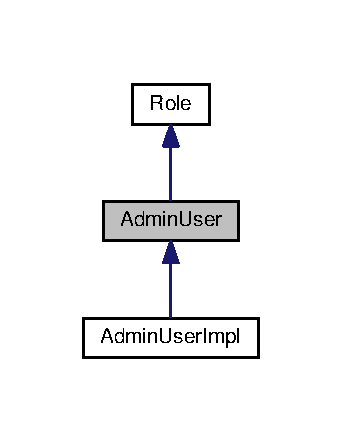
\includegraphics[width=164pt]{d1/d65/classAdminUser__inherit__graph}
\end{center}
\end{figure}


Collaboration diagram for Admin\+User\+:
\nopagebreak
\begin{figure}[H]
\begin{center}
\leavevmode
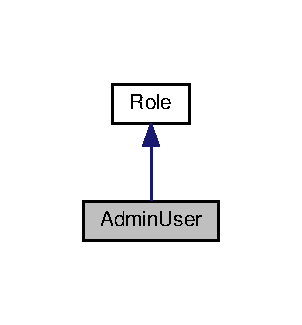
\includegraphics[width=145pt]{d4/d52/classAdminUser__coll__graph}
\end{center}
\end{figure}
\subsection*{Public Member Functions}
\begin{DoxyCompactItemize}
\item 
virtual Q\+String \hyperlink{classAdminUser_adc74bc08cca80fed7a0e0a7c7be596b3}{get\+Username} ()=0
\begin{DoxyCompactList}\small\item\em Método para acessa o nome do usuário correspondente. \end{DoxyCompactList}\end{DoxyCompactItemize}
\subsection*{Static Public Attributes}
\begin{DoxyCompactItemize}
\item 
static const Q\+String \hyperlink{classAdminUser_a91f12ea178ac4cc117cb5eb8d5cd9053}{A\+D\+M\+I\+N\+\_\+\+U\+S\+E\+R\+\_\+\+N\+A\+ME} = \char`\"{}Admin\char`\"{}\hypertarget{classAdminUser_a91f12ea178ac4cc117cb5eb8d5cd9053}{}\label{classAdminUser_a91f12ea178ac4cc117cb5eb8d5cd9053}

\begin{DoxyCompactList}\small\item\em Nome do papel \char`\"{}\+Administrador\char`\"{}. \end{DoxyCompactList}\end{DoxyCompactItemize}


\subsection{Detailed Description}
Interface correspondente ao papel de administrador do sistema. 

\subsection{Member Function Documentation}
\index{Admin\+User@{Admin\+User}!get\+Username@{get\+Username}}
\index{get\+Username@{get\+Username}!Admin\+User@{Admin\+User}}
\subsubsection[{\texorpdfstring{get\+Username()=0}{getUsername()=0}}]{\setlength{\rightskip}{0pt plus 5cm}virtual Q\+String Admin\+User\+::get\+Username (
\begin{DoxyParamCaption}
{}
\end{DoxyParamCaption}
)\hspace{0.3cm}{\ttfamily [pure virtual]}}\hypertarget{classAdminUser_adc74bc08cca80fed7a0e0a7c7be596b3}{}\label{classAdminUser_adc74bc08cca80fed7a0e0a7c7be596b3}


Método para acessa o nome do usuário correspondente. 

\begin{DoxyReturn}{Returns}
Nome do usuário 
\end{DoxyReturn}


Implemented in \hyperlink{classAdminUserImpl_af66494cfe7eecb1199cfc3295c009f2c}{Admin\+User\+Impl}.



The documentation for this class was generated from the following files\+:\begin{DoxyCompactItemize}
\item 
Calc\+Client/src/data/\hyperlink{adminuser_8h}{adminuser.\+h}\item 
Calc\+Client/src/data/\hyperlink{adminuserimpl_8cpp}{adminuserimpl.\+cpp}\end{DoxyCompactItemize}

\hypertarget{classAdminUserImpl}{}\section{Admin\+User\+Impl Class Reference}
\label{classAdminUserImpl}\index{Admin\+User\+Impl@{Admin\+User\+Impl}}


Implementação da Interface \hyperlink{classAdminUser}{Admin\+User}.  




{\ttfamily \#include $<$adminuserimpl.\+h$>$}



Inheritance diagram for Admin\+User\+Impl\+:
\nopagebreak
\begin{figure}[H]
\begin{center}
\leavevmode
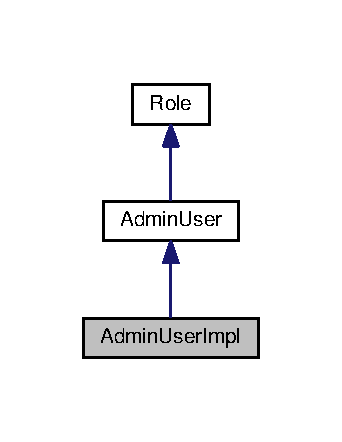
\includegraphics[width=164pt]{d6/d85/classAdminUserImpl__inherit__graph}
\end{center}
\end{figure}


Collaboration diagram for Admin\+User\+Impl\+:
\nopagebreak
\begin{figure}[H]
\begin{center}
\leavevmode
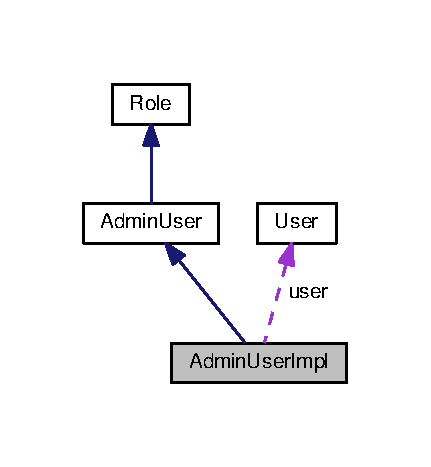
\includegraphics[width=207pt]{df/dc0/classAdminUserImpl__coll__graph}
\end{center}
\end{figure}
\subsection*{Public Member Functions}
\begin{DoxyCompactItemize}
\item 
\hyperlink{classAdminUserImpl_a45371b972d5cd8feaa8c3cd592761f8c}{Admin\+User\+Impl} ()\hypertarget{classAdminUserImpl_a45371b972d5cd8feaa8c3cd592761f8c}{}\label{classAdminUserImpl_a45371b972d5cd8feaa8c3cd592761f8c}

\begin{DoxyCompactList}\small\item\em Construtor padrão. \end{DoxyCompactList}\item 
virtual Q\+String \hyperlink{classAdminUserImpl_af66494cfe7eecb1199cfc3295c009f2c}{get\+Username} () override
\begin{DoxyCompactList}\small\item\em Método para acessa o nome do usuário correspondente. \end{DoxyCompactList}\item 
virtual Q\+String \hyperlink{classAdminUserImpl_a8fc6881cf92e783065001be43209a5a6}{get\+Role\+Name} () override
\begin{DoxyCompactList}\small\item\em Método para acessar o nome papel. \end{DoxyCompactList}\item 
virtual \hyperlink{classUser}{User} $\ast$ \hyperlink{classAdminUserImpl_aa548616e5bf99062155ee397bf9be6ad}{get\+User} () override
\begin{DoxyCompactList}\small\item\em Método para acessar o usuário correspondente ao papel. \end{DoxyCompactList}\item 
virtual void \hyperlink{classAdminUserImpl_a5a392bdfba62518e31e40819fe3c32b7}{set\+User} (\hyperlink{classUser}{User} $\ast$\hyperlink{classAdminUserImpl_af88f707a7bd759f9613ab55c29767cc2}{user}) override
\begin{DoxyCompactList}\small\item\em Método para associar um usuário a um papel. \end{DoxyCompactList}\end{DoxyCompactItemize}
\subsection*{Private Attributes}
\begin{DoxyCompactItemize}
\item 
\hyperlink{classUser}{User} $\ast$ \hyperlink{classAdminUserImpl_af88f707a7bd759f9613ab55c29767cc2}{user}\hypertarget{classAdminUserImpl_af88f707a7bd759f9613ab55c29767cc2}{}\label{classAdminUserImpl_af88f707a7bd759f9613ab55c29767cc2}

\begin{DoxyCompactList}\small\item\em Ponteiro para o usuário correspondente a este papel. \end{DoxyCompactList}\end{DoxyCompactItemize}
\subsection*{Additional Inherited Members}


\subsection{Detailed Description}
Implementação da Interface \hyperlink{classAdminUser}{Admin\+User}. 

\subsection{Member Function Documentation}
\index{Admin\+User\+Impl@{Admin\+User\+Impl}!get\+Role\+Name@{get\+Role\+Name}}
\index{get\+Role\+Name@{get\+Role\+Name}!Admin\+User\+Impl@{Admin\+User\+Impl}}
\subsubsection[{\texorpdfstring{get\+Role\+Name() override}{getRoleName() override}}]{\setlength{\rightskip}{0pt plus 5cm}Q\+String Admin\+User\+Impl\+::get\+Role\+Name (
\begin{DoxyParamCaption}
{}
\end{DoxyParamCaption}
)\hspace{0.3cm}{\ttfamily [override]}, {\ttfamily [virtual]}}\hypertarget{classAdminUserImpl_a8fc6881cf92e783065001be43209a5a6}{}\label{classAdminUserImpl_a8fc6881cf92e783065001be43209a5a6}


Método para acessar o nome papel. 

\begin{DoxyReturn}{Returns}
Nome do papel 
\end{DoxyReturn}


Implements \hyperlink{classRole_a295daeaed997d10f9bd3d03e972318c1}{Role}.

\index{Admin\+User\+Impl@{Admin\+User\+Impl}!get\+User@{get\+User}}
\index{get\+User@{get\+User}!Admin\+User\+Impl@{Admin\+User\+Impl}}
\subsubsection[{\texorpdfstring{get\+User() override}{getUser() override}}]{\setlength{\rightskip}{0pt plus 5cm}{\bf User} $\ast$ Admin\+User\+Impl\+::get\+User (
\begin{DoxyParamCaption}
{}
\end{DoxyParamCaption}
)\hspace{0.3cm}{\ttfamily [override]}, {\ttfamily [virtual]}}\hypertarget{classAdminUserImpl_aa548616e5bf99062155ee397bf9be6ad}{}\label{classAdminUserImpl_aa548616e5bf99062155ee397bf9be6ad}


Método para acessar o usuário correspondente ao papel. 

\begin{DoxyReturn}{Returns}
Usuário associado ao papel 
\end{DoxyReturn}


Implements \hyperlink{classRole_abad7de00bc38b11eaae8a79069773221}{Role}.

\index{Admin\+User\+Impl@{Admin\+User\+Impl}!get\+Username@{get\+Username}}
\index{get\+Username@{get\+Username}!Admin\+User\+Impl@{Admin\+User\+Impl}}
\subsubsection[{\texorpdfstring{get\+Username() override}{getUsername() override}}]{\setlength{\rightskip}{0pt plus 5cm}Q\+String Admin\+User\+Impl\+::get\+Username (
\begin{DoxyParamCaption}
{}
\end{DoxyParamCaption}
)\hspace{0.3cm}{\ttfamily [override]}, {\ttfamily [virtual]}}\hypertarget{classAdminUserImpl_af66494cfe7eecb1199cfc3295c009f2c}{}\label{classAdminUserImpl_af66494cfe7eecb1199cfc3295c009f2c}


Método para acessa o nome do usuário correspondente. 

\begin{DoxyReturn}{Returns}
Nome do usuário 
\end{DoxyReturn}


Implements \hyperlink{classAdminUser_adc74bc08cca80fed7a0e0a7c7be596b3}{Admin\+User}.

\index{Admin\+User\+Impl@{Admin\+User\+Impl}!set\+User@{set\+User}}
\index{set\+User@{set\+User}!Admin\+User\+Impl@{Admin\+User\+Impl}}
\subsubsection[{\texorpdfstring{set\+User(\+User $\ast$user) override}{setUser(User *user) override}}]{\setlength{\rightskip}{0pt plus 5cm}void Admin\+User\+Impl\+::set\+User (
\begin{DoxyParamCaption}
\item[{{\bf User} $\ast$}]{user}
\end{DoxyParamCaption}
)\hspace{0.3cm}{\ttfamily [override]}, {\ttfamily [virtual]}}\hypertarget{classAdminUserImpl_a5a392bdfba62518e31e40819fe3c32b7}{}\label{classAdminUserImpl_a5a392bdfba62518e31e40819fe3c32b7}


Método para associar um usuário a um papel. 


\begin{DoxyParams}{Parameters}
{\em user} & Usuário a ser associado \\
\hline
\end{DoxyParams}


Implements \hyperlink{classRole_ab5581d91192fa578070e80b0247dde5a}{Role}.



The documentation for this class was generated from the following files\+:\begin{DoxyCompactItemize}
\item 
Calc\+Client/src/data/\hyperlink{adminuserimpl_8h}{adminuserimpl.\+h}\item 
Calc\+Client/src/data/\hyperlink{adminuserimpl_8cpp}{adminuserimpl.\+cpp}\end{DoxyCompactItemize}

\hypertarget{classBasicUser}{}\section{Basic\+User Class Reference}
\label{classBasicUser}\index{Basic\+User@{Basic\+User}}


Interface correspondente ao papel usuário.  




{\ttfamily \#include $<$basicuser.\+h$>$}



Inheritance diagram for Basic\+User\+:
\nopagebreak
\begin{figure}[H]
\begin{center}
\leavevmode
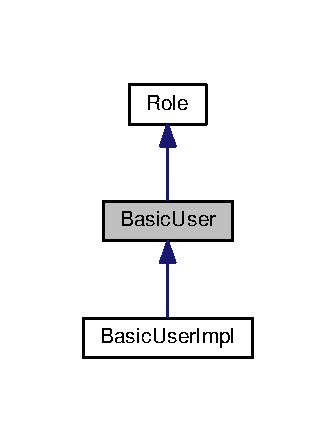
\includegraphics[width=161pt]{d5/d46/classBasicUser__inherit__graph}
\end{center}
\end{figure}


Collaboration diagram for Basic\+User\+:
\nopagebreak
\begin{figure}[H]
\begin{center}
\leavevmode
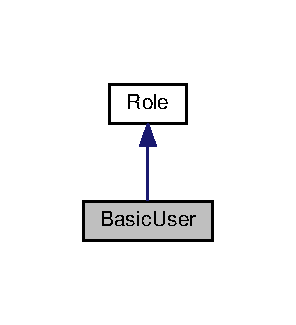
\includegraphics[width=142pt]{de/d6b/classBasicUser__coll__graph}
\end{center}
\end{figure}
\subsection*{Public Member Functions}
\begin{DoxyCompactItemize}
\item 
virtual Q\+String \hyperlink{classBasicUser_ae5ed7101550b9c9d280df5adf030975d}{get\+Username} ()=0
\begin{DoxyCompactList}\small\item\em Acessa o nome do usuário. \end{DoxyCompactList}\item 
virtual Q\+String \hyperlink{classBasicUser_a240bd2f9974357c921a79499355b1e18}{get\+Password} ()=0
\begin{DoxyCompactList}\small\item\em Acessa a senha do usuário. \end{DoxyCompactList}\end{DoxyCompactItemize}
\subsection*{Static Public Attributes}
\begin{DoxyCompactItemize}
\item 
static const Q\+String \hyperlink{classBasicUser_aaaea5b09e42b753e0ea0331797a48a3f}{B\+A\+S\+I\+C\+\_\+\+U\+S\+E\+R\+\_\+\+N\+A\+ME} = \char`\"{}User\char`\"{}\hypertarget{classBasicUser_aaaea5b09e42b753e0ea0331797a48a3f}{}\label{classBasicUser_aaaea5b09e42b753e0ea0331797a48a3f}

\begin{DoxyCompactList}\small\item\em Nome do papel \char`\"{}\+Usuário\char`\"{}. \end{DoxyCompactList}\end{DoxyCompactItemize}


\subsection{Detailed Description}
Interface correspondente ao papel usuário. 

\subsection{Member Function Documentation}
\index{Basic\+User@{Basic\+User}!get\+Password@{get\+Password}}
\index{get\+Password@{get\+Password}!Basic\+User@{Basic\+User}}
\subsubsection[{\texorpdfstring{get\+Password()=0}{getPassword()=0}}]{\setlength{\rightskip}{0pt plus 5cm}virtual Q\+String Basic\+User\+::get\+Password (
\begin{DoxyParamCaption}
{}
\end{DoxyParamCaption}
)\hspace{0.3cm}{\ttfamily [pure virtual]}}\hypertarget{classBasicUser_a240bd2f9974357c921a79499355b1e18}{}\label{classBasicUser_a240bd2f9974357c921a79499355b1e18}


Acessa a senha do usuário. 

\begin{DoxyReturn}{Returns}
Senha do usuário 
\end{DoxyReturn}


Implemented in \hyperlink{classBasicUserImpl_a94c89958edd477672063ba246ef77f8a}{Basic\+User\+Impl}.

\index{Basic\+User@{Basic\+User}!get\+Username@{get\+Username}}
\index{get\+Username@{get\+Username}!Basic\+User@{Basic\+User}}
\subsubsection[{\texorpdfstring{get\+Username()=0}{getUsername()=0}}]{\setlength{\rightskip}{0pt plus 5cm}virtual Q\+String Basic\+User\+::get\+Username (
\begin{DoxyParamCaption}
{}
\end{DoxyParamCaption}
)\hspace{0.3cm}{\ttfamily [pure virtual]}}\hypertarget{classBasicUser_ae5ed7101550b9c9d280df5adf030975d}{}\label{classBasicUser_ae5ed7101550b9c9d280df5adf030975d}


Acessa o nome do usuário. 

\begin{DoxyReturn}{Returns}
Nome do usuário 
\end{DoxyReturn}


Implemented in \hyperlink{classBasicUserImpl_ad5c2ba5c4d7b179e12f25ad843544de0}{Basic\+User\+Impl}.



The documentation for this class was generated from the following files\+:\begin{DoxyCompactItemize}
\item 
Calc\+Client/src/data/\hyperlink{basicuser_8h}{basicuser.\+h}\item 
Calc\+Client/src/data/\hyperlink{basicuserimpl_8cpp}{basicuserimpl.\+cpp}\end{DoxyCompactItemize}

\hypertarget{classBasicUserImpl}{}\section{Basic\+User\+Impl Class Reference}
\label{classBasicUserImpl}\index{Basic\+User\+Impl@{Basic\+User\+Impl}}


Implementação da interface \hyperlink{classBasicUser}{Basic\+User}.  




{\ttfamily \#include $<$basicuserimpl.\+h$>$}



Inheritance diagram for Basic\+User\+Impl\+:
\nopagebreak
\begin{figure}[H]
\begin{center}
\leavevmode
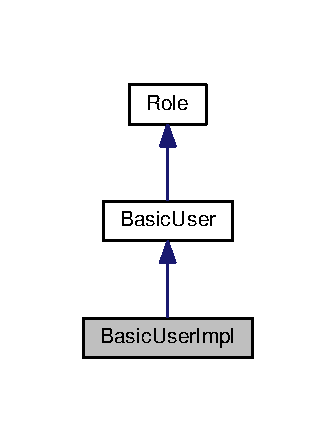
\includegraphics[width=161pt]{de/d1f/classBasicUserImpl__inherit__graph}
\end{center}
\end{figure}


Collaboration diagram for Basic\+User\+Impl\+:
\nopagebreak
\begin{figure}[H]
\begin{center}
\leavevmode
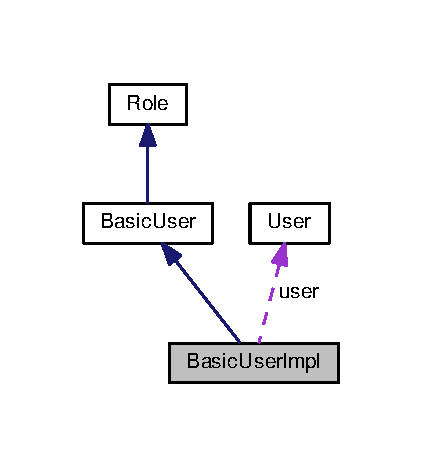
\includegraphics[width=203pt]{d7/dcb/classBasicUserImpl__coll__graph}
\end{center}
\end{figure}
\subsection*{Public Member Functions}
\begin{DoxyCompactItemize}
\item 
\hyperlink{classBasicUserImpl_a833561b430281e72ab7ba48ab3d7b749}{Basic\+User\+Impl} ()\hypertarget{classBasicUserImpl_a833561b430281e72ab7ba48ab3d7b749}{}\label{classBasicUserImpl_a833561b430281e72ab7ba48ab3d7b749}

\begin{DoxyCompactList}\small\item\em Construtor padrão. \end{DoxyCompactList}\item 
virtual Q\+String \hyperlink{classBasicUserImpl_aaf68b785533f15a61fa30cdef3c82145}{get\+Role\+Name} () override
\begin{DoxyCompactList}\small\item\em Método para acessar o nome papel. \end{DoxyCompactList}\item 
virtual \hyperlink{classUser}{User} $\ast$ \hyperlink{classBasicUserImpl_ace1ba87379b0b3817a089d6933dc0dd7}{get\+User} () override
\begin{DoxyCompactList}\small\item\em Método para acessar o usuário correspondente ao papel. \end{DoxyCompactList}\item 
virtual void \hyperlink{classBasicUserImpl_af94875b3b06f1f1effc3a58fce087e5d}{set\+User} (\hyperlink{classUser}{User} $\ast$\hyperlink{classBasicUserImpl_a1c6cfd2fe227c0eae9bdded2afecf1ec}{user}) override
\begin{DoxyCompactList}\small\item\em Método para associar um usuário a um papel. \end{DoxyCompactList}\item 
virtual Q\+String \hyperlink{classBasicUserImpl_ad5c2ba5c4d7b179e12f25ad843544de0}{get\+Username} () override
\begin{DoxyCompactList}\small\item\em Acessa o nome do usuário. \end{DoxyCompactList}\item 
virtual Q\+String \hyperlink{classBasicUserImpl_a94c89958edd477672063ba246ef77f8a}{get\+Password} () override
\begin{DoxyCompactList}\small\item\em Acessa a senha do usuário. \end{DoxyCompactList}\end{DoxyCompactItemize}
\subsection*{Private Attributes}
\begin{DoxyCompactItemize}
\item 
\hyperlink{classUser}{User} $\ast$ \hyperlink{classBasicUserImpl_a1c6cfd2fe227c0eae9bdded2afecf1ec}{user}\hypertarget{classBasicUserImpl_a1c6cfd2fe227c0eae9bdded2afecf1ec}{}\label{classBasicUserImpl_a1c6cfd2fe227c0eae9bdded2afecf1ec}

\begin{DoxyCompactList}\small\item\em Ponteiro para o usuário correspondente a este papel. \end{DoxyCompactList}\end{DoxyCompactItemize}
\subsection*{Additional Inherited Members}


\subsection{Detailed Description}
Implementação da interface \hyperlink{classBasicUser}{Basic\+User}. 

\subsection{Member Function Documentation}
\index{Basic\+User\+Impl@{Basic\+User\+Impl}!get\+Password@{get\+Password}}
\index{get\+Password@{get\+Password}!Basic\+User\+Impl@{Basic\+User\+Impl}}
\subsubsection[{\texorpdfstring{get\+Password() override}{getPassword() override}}]{\setlength{\rightskip}{0pt plus 5cm}Q\+String Basic\+User\+Impl\+::get\+Password (
\begin{DoxyParamCaption}
{}
\end{DoxyParamCaption}
)\hspace{0.3cm}{\ttfamily [override]}, {\ttfamily [virtual]}}\hypertarget{classBasicUserImpl_a94c89958edd477672063ba246ef77f8a}{}\label{classBasicUserImpl_a94c89958edd477672063ba246ef77f8a}


Acessa a senha do usuário. 

\begin{DoxyReturn}{Returns}
Senha do usuário 
\end{DoxyReturn}


Implements \hyperlink{classBasicUser_a240bd2f9974357c921a79499355b1e18}{Basic\+User}.

\index{Basic\+User\+Impl@{Basic\+User\+Impl}!get\+Role\+Name@{get\+Role\+Name}}
\index{get\+Role\+Name@{get\+Role\+Name}!Basic\+User\+Impl@{Basic\+User\+Impl}}
\subsubsection[{\texorpdfstring{get\+Role\+Name() override}{getRoleName() override}}]{\setlength{\rightskip}{0pt plus 5cm}Q\+String Basic\+User\+Impl\+::get\+Role\+Name (
\begin{DoxyParamCaption}
{}
\end{DoxyParamCaption}
)\hspace{0.3cm}{\ttfamily [override]}, {\ttfamily [virtual]}}\hypertarget{classBasicUserImpl_aaf68b785533f15a61fa30cdef3c82145}{}\label{classBasicUserImpl_aaf68b785533f15a61fa30cdef3c82145}


Método para acessar o nome papel. 

\begin{DoxyReturn}{Returns}
Nome do papel 
\end{DoxyReturn}


Implements \hyperlink{classRole_a295daeaed997d10f9bd3d03e972318c1}{Role}.

\index{Basic\+User\+Impl@{Basic\+User\+Impl}!get\+User@{get\+User}}
\index{get\+User@{get\+User}!Basic\+User\+Impl@{Basic\+User\+Impl}}
\subsubsection[{\texorpdfstring{get\+User() override}{getUser() override}}]{\setlength{\rightskip}{0pt plus 5cm}{\bf User} $\ast$ Basic\+User\+Impl\+::get\+User (
\begin{DoxyParamCaption}
{}
\end{DoxyParamCaption}
)\hspace{0.3cm}{\ttfamily [override]}, {\ttfamily [virtual]}}\hypertarget{classBasicUserImpl_ace1ba87379b0b3817a089d6933dc0dd7}{}\label{classBasicUserImpl_ace1ba87379b0b3817a089d6933dc0dd7}


Método para acessar o usuário correspondente ao papel. 

\begin{DoxyReturn}{Returns}
Usuário associado ao papel 
\end{DoxyReturn}


Implements \hyperlink{classRole_abad7de00bc38b11eaae8a79069773221}{Role}.

\index{Basic\+User\+Impl@{Basic\+User\+Impl}!get\+Username@{get\+Username}}
\index{get\+Username@{get\+Username}!Basic\+User\+Impl@{Basic\+User\+Impl}}
\subsubsection[{\texorpdfstring{get\+Username() override}{getUsername() override}}]{\setlength{\rightskip}{0pt plus 5cm}Q\+String Basic\+User\+Impl\+::get\+Username (
\begin{DoxyParamCaption}
{}
\end{DoxyParamCaption}
)\hspace{0.3cm}{\ttfamily [override]}, {\ttfamily [virtual]}}\hypertarget{classBasicUserImpl_ad5c2ba5c4d7b179e12f25ad843544de0}{}\label{classBasicUserImpl_ad5c2ba5c4d7b179e12f25ad843544de0}


Acessa o nome do usuário. 

\begin{DoxyReturn}{Returns}
Nome do usuário 
\end{DoxyReturn}


Implements \hyperlink{classBasicUser_ae5ed7101550b9c9d280df5adf030975d}{Basic\+User}.

\index{Basic\+User\+Impl@{Basic\+User\+Impl}!set\+User@{set\+User}}
\index{set\+User@{set\+User}!Basic\+User\+Impl@{Basic\+User\+Impl}}
\subsubsection[{\texorpdfstring{set\+User(\+User $\ast$user) override}{setUser(User *user) override}}]{\setlength{\rightskip}{0pt plus 5cm}void Basic\+User\+Impl\+::set\+User (
\begin{DoxyParamCaption}
\item[{{\bf User} $\ast$}]{user}
\end{DoxyParamCaption}
)\hspace{0.3cm}{\ttfamily [override]}, {\ttfamily [virtual]}}\hypertarget{classBasicUserImpl_af94875b3b06f1f1effc3a58fce087e5d}{}\label{classBasicUserImpl_af94875b3b06f1f1effc3a58fce087e5d}


Método para associar um usuário a um papel. 


\begin{DoxyParams}{Parameters}
{\em user} & Usuário a ser associado \\
\hline
\end{DoxyParams}


Implements \hyperlink{classRole_ab5581d91192fa578070e80b0247dde5a}{Role}.



The documentation for this class was generated from the following files\+:\begin{DoxyCompactItemize}
\item 
Calc\+Client/src/data/\hyperlink{basicuserimpl_8h}{basicuserimpl.\+h}\item 
Calc\+Client/src/data/\hyperlink{basicuserimpl_8cpp}{basicuserimpl.\+cpp}\end{DoxyCompactItemize}

\hypertarget{classDatabaseHelper}{}\section{Database\+Helper Class Reference}
\label{classDatabaseHelper}\index{Database\+Helper@{Database\+Helper}}


Interface para acesso a um banco de dados.  




{\ttfamily \#include $<$databasehelper.\+h$>$}



Inheritance diagram for Database\+Helper\+:
\nopagebreak
\begin{figure}[H]
\begin{center}
\leavevmode
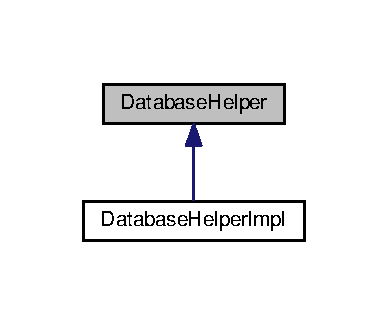
\includegraphics[width=186pt]{d0/dc0/classDatabaseHelper__inherit__graph}
\end{center}
\end{figure}
\subsection*{Public Member Functions}
\begin{DoxyCompactItemize}
\item 
virtual int \hyperlink{classDatabaseHelper_a03e499b83f152466abed94fef2f0ef73}{get\+User\+Id} (Q\+String username)=0
\begin{DoxyCompactList}\small\item\em Esse método busca se um usuário está presente no banco de dados. \end{DoxyCompactList}\item 
virtual bool \hyperlink{classDatabaseHelper_aaff1d6157ea2d4fa7edb6744e8ce7daf}{insert\+Operation} (int user\+Id, double v1, Q\+String operacao, double v2, double resultado)=0
\begin{DoxyCompactList}\small\item\em Esse método armazena um registro de operação. \end{DoxyCompactList}\item 
virtual vector$<$ pair$<$ Q\+String, Q\+String $>$ $>$ \hyperlink{classDatabaseHelper_a32fe64f07291bbefc59e92690b7017bf}{get\+All\+Users} ()=0
\begin{DoxyCompactList}\small\item\em Retorna todos os usuários do banco e seus respectivas senhas. \end{DoxyCompactList}\item 
virtual vector$<$ pair$<$ Q\+String, int $>$ $>$ \hyperlink{classDatabaseHelper_ae9b9e741f7a776348dd334de3fa7e52b}{get\+Operations\+By\+User} (Q\+String username)=0
\begin{DoxyCompactList}\small\item\em Gera uma tabela de sobre as operações realizadas pelo usuário. \end{DoxyCompactList}\item 
virtual vector$<$ pair$<$ Q\+String, int $>$ $>$ \hyperlink{classDatabaseHelper_adc20c023d6dd87602bfd3310bddcf6d1}{get\+All\+Operations} ()=0
\begin{DoxyCompactList}\small\item\em Gera uma tabela de sobre as operações realizadas por todos os usuários. \end{DoxyCompactList}\item 
virtual bool \hyperlink{classDatabaseHelper_aca0024be103d394caf3a6eef7899c714}{is\+Admin} (Q\+String username)=0
\begin{DoxyCompactList}\small\item\em Verifica se um usuário tem permissõe de administrador. \end{DoxyCompactList}\end{DoxyCompactItemize}


\subsection{Detailed Description}
Interface para acesso a um banco de dados. 

\subsection{Member Function Documentation}
\index{Database\+Helper@{Database\+Helper}!get\+All\+Operations@{get\+All\+Operations}}
\index{get\+All\+Operations@{get\+All\+Operations}!Database\+Helper@{Database\+Helper}}
\subsubsection[{\texorpdfstring{get\+All\+Operations()=0}{getAllOperations()=0}}]{\setlength{\rightskip}{0pt plus 5cm}virtual vector$<$pair$<$Q\+String, int$>$ $>$ Database\+Helper\+::get\+All\+Operations (
\begin{DoxyParamCaption}
{}
\end{DoxyParamCaption}
)\hspace{0.3cm}{\ttfamily [pure virtual]}}\hypertarget{classDatabaseHelper_adc20c023d6dd87602bfd3310bddcf6d1}{}\label{classDatabaseHelper_adc20c023d6dd87602bfd3310bddcf6d1}


Gera uma tabela de sobre as operações realizadas por todos os usuários. 

\begin{DoxyReturn}{Returns}
Lista de pares contendo tipo de operação e quantidade de vezes que ela foi realizada. 
\end{DoxyReturn}
\begin{DoxySeeAlso}{See also}
\hyperlink{classDatabaseHelper_ae9b9e741f7a776348dd334de3fa7e52b}{Database\+Helper\+::get\+Operations\+By\+User(\+Q\+String)}. 
\end{DoxySeeAlso}


Implemented in \hyperlink{classDatabaseHelperImpl_aedd37d515fad4f0b0884748bf77f677c}{Database\+Helper\+Impl}.

\index{Database\+Helper@{Database\+Helper}!get\+All\+Users@{get\+All\+Users}}
\index{get\+All\+Users@{get\+All\+Users}!Database\+Helper@{Database\+Helper}}
\subsubsection[{\texorpdfstring{get\+All\+Users()=0}{getAllUsers()=0}}]{\setlength{\rightskip}{0pt plus 5cm}virtual vector$<$pair$<$Q\+String, Q\+String$>$ $>$ Database\+Helper\+::get\+All\+Users (
\begin{DoxyParamCaption}
{}
\end{DoxyParamCaption}
)\hspace{0.3cm}{\ttfamily [pure virtual]}}\hypertarget{classDatabaseHelper_a32fe64f07291bbefc59e92690b7017bf}{}\label{classDatabaseHelper_a32fe64f07291bbefc59e92690b7017bf}


Retorna todos os usuários do banco e seus respectivas senhas. 

\begin{DoxyReturn}{Returns}
Lista de pares contendo nome de usuário e senha. 
\end{DoxyReturn}


Implemented in \hyperlink{classDatabaseHelperImpl_ac93f23c05d794595149585c451f24605}{Database\+Helper\+Impl}.

\index{Database\+Helper@{Database\+Helper}!get\+Operations\+By\+User@{get\+Operations\+By\+User}}
\index{get\+Operations\+By\+User@{get\+Operations\+By\+User}!Database\+Helper@{Database\+Helper}}
\subsubsection[{\texorpdfstring{get\+Operations\+By\+User(\+Q\+String username)=0}{getOperationsByUser(QString username)=0}}]{\setlength{\rightskip}{0pt plus 5cm}virtual vector$<$pair$<$Q\+String, int$>$ $>$ Database\+Helper\+::get\+Operations\+By\+User (
\begin{DoxyParamCaption}
\item[{Q\+String}]{username}
\end{DoxyParamCaption}
)\hspace{0.3cm}{\ttfamily [pure virtual]}}\hypertarget{classDatabaseHelper_ae9b9e741f7a776348dd334de3fa7e52b}{}\label{classDatabaseHelper_ae9b9e741f7a776348dd334de3fa7e52b}


Gera uma tabela de sobre as operações realizadas pelo usuário. 


\begin{DoxyParams}{Parameters}
{\em username} & Nome do usuário a ser buscado. \\
\hline
\end{DoxyParams}
\begin{DoxyReturn}{Returns}
Lista de pares contendo tipo de operação e quantidade de vezes que ela foi realizada. 
\end{DoxyReturn}
\begin{DoxySeeAlso}{See also}
\hyperlink{classDatabaseHelper_adc20c023d6dd87602bfd3310bddcf6d1}{Database\+Helper\+::get\+All\+Operations()}. 
\end{DoxySeeAlso}


Implemented in \hyperlink{classDatabaseHelperImpl_a124bd600c3e2daa19dc24982eb3dea14}{Database\+Helper\+Impl}.

\index{Database\+Helper@{Database\+Helper}!get\+User\+Id@{get\+User\+Id}}
\index{get\+User\+Id@{get\+User\+Id}!Database\+Helper@{Database\+Helper}}
\subsubsection[{\texorpdfstring{get\+User\+Id(\+Q\+String username)=0}{getUserId(QString username)=0}}]{\setlength{\rightskip}{0pt plus 5cm}virtual int Database\+Helper\+::get\+User\+Id (
\begin{DoxyParamCaption}
\item[{Q\+String}]{username}
\end{DoxyParamCaption}
)\hspace{0.3cm}{\ttfamily [pure virtual]}}\hypertarget{classDatabaseHelper_a03e499b83f152466abed94fef2f0ef73}{}\label{classDatabaseHelper_a03e499b83f152466abed94fef2f0ef73}


Esse método busca se um usuário está presente no banco de dados. 


\begin{DoxyParams}{Parameters}
{\em username} & Nome do usuário a ser buscado. \\
\hline
\end{DoxyParams}
\begin{DoxyReturn}{Returns}
O id do usuário no banco. 
\end{DoxyReturn}


Implemented in \hyperlink{classDatabaseHelperImpl_a071ca71dc50d21a3d5749156aec99476}{Database\+Helper\+Impl}.

\index{Database\+Helper@{Database\+Helper}!insert\+Operation@{insert\+Operation}}
\index{insert\+Operation@{insert\+Operation}!Database\+Helper@{Database\+Helper}}
\subsubsection[{\texorpdfstring{insert\+Operation(int user\+Id, double v1, Q\+String operacao, double v2, double resultado)=0}{insertOperation(int userId, double v1, QString operacao, double v2, double resultado)=0}}]{\setlength{\rightskip}{0pt plus 5cm}virtual bool Database\+Helper\+::insert\+Operation (
\begin{DoxyParamCaption}
\item[{int}]{user\+Id, }
\item[{double}]{v1, }
\item[{Q\+String}]{operacao, }
\item[{double}]{v2, }
\item[{double}]{resultado}
\end{DoxyParamCaption}
)\hspace{0.3cm}{\ttfamily [pure virtual]}}\hypertarget{classDatabaseHelper_aaff1d6157ea2d4fa7edb6744e8ce7daf}{}\label{classDatabaseHelper_aaff1d6157ea2d4fa7edb6744e8ce7daf}


Esse método armazena um registro de operação. 


\begin{DoxyParams}{Parameters}
{\em user\+Id} & Id do usuário que realizou a operação. \\
\hline
{\em v1} & Primeiro operando. \\
\hline
{\em operacao} & Operação realizada. \\
\hline
{\em v2} & Segundo Operando. \\
\hline
{\em resultado} & Resultado da operação. \\
\hline
\end{DoxyParams}
\begin{DoxyReturn}{Returns}
Se a inserção foi realizada. 
\end{DoxyReturn}


Implemented in \hyperlink{classDatabaseHelperImpl_a4791d584b178b71a186a843dbc8ab86e}{Database\+Helper\+Impl}.

\index{Database\+Helper@{Database\+Helper}!is\+Admin@{is\+Admin}}
\index{is\+Admin@{is\+Admin}!Database\+Helper@{Database\+Helper}}
\subsubsection[{\texorpdfstring{is\+Admin(\+Q\+String username)=0}{isAdmin(QString username)=0}}]{\setlength{\rightskip}{0pt plus 5cm}virtual bool Database\+Helper\+::is\+Admin (
\begin{DoxyParamCaption}
\item[{Q\+String}]{username}
\end{DoxyParamCaption}
)\hspace{0.3cm}{\ttfamily [pure virtual]}}\hypertarget{classDatabaseHelper_aca0024be103d394caf3a6eef7899c714}{}\label{classDatabaseHelper_aca0024be103d394caf3a6eef7899c714}


Verifica se um usuário tem permissõe de administrador. 


\begin{DoxyParams}{Parameters}
{\em username} & Nome do usuário a ser buscado. \\
\hline
\end{DoxyParams}
\begin{DoxyReturn}{Returns}
Se o usuário é administrador. 
\end{DoxyReturn}


Implemented in \hyperlink{classDatabaseHelperImpl_a3c6da9438b26955fcef6a080c85652f5}{Database\+Helper\+Impl}.



The documentation for this class was generated from the following file\+:\begin{DoxyCompactItemize}
\item 
Calc\+Server/src/database/\hyperlink{databasehelper_8h}{databasehelper.\+h}\end{DoxyCompactItemize}

\hypertarget{classDatabaseHelperImpl}{}\section{Database\+Helper\+Impl Class Reference}
\label{classDatabaseHelperImpl}\index{Database\+Helper\+Impl@{Database\+Helper\+Impl}}


Implementação da Interface \hyperlink{classDatabaseHelper}{Database\+Helper} para acesso ao banco de dados S\+Q\+Lite.  




{\ttfamily \#include $<$databasehelperimpl.\+h$>$}



Inheritance diagram for Database\+Helper\+Impl\+:\nopagebreak
\begin{figure}[H]
\begin{center}
\leavevmode
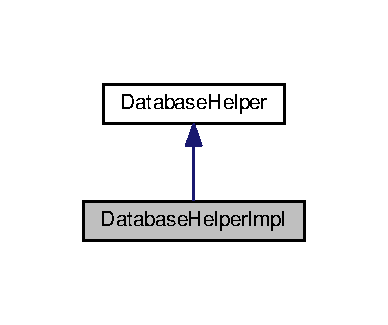
\includegraphics[width=186pt]{dd/d1d/classDatabaseHelperImpl__inherit__graph}
\end{center}
\end{figure}


Collaboration diagram for Database\+Helper\+Impl\+:\nopagebreak
\begin{figure}[H]
\begin{center}
\leavevmode
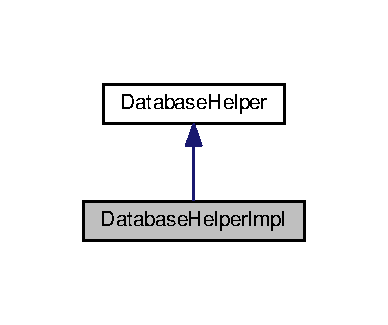
\includegraphics[width=186pt]{d8/da4/classDatabaseHelperImpl__coll__graph}
\end{center}
\end{figure}
\subsection*{Public Member Functions}
\begin{DoxyCompactItemize}
\item 
\hyperlink{classDatabaseHelperImpl_a60f67f9c6183e02ffab826bf254fef10}{Database\+Helper\+Impl} ()\hypertarget{classDatabaseHelperImpl_a60f67f9c6183e02ffab826bf254fef10}{}\label{classDatabaseHelperImpl_a60f67f9c6183e02ffab826bf254fef10}

\begin{DoxyCompactList}\small\item\em Construtor padrão. \end{DoxyCompactList}\item 
virtual \hyperlink{classDatabaseHelperImpl_a14d7fa4590316828d2e802bff3512223}{$\sim$\+Database\+Helper\+Impl} ()\hypertarget{classDatabaseHelperImpl_a14d7fa4590316828d2e802bff3512223}{}\label{classDatabaseHelperImpl_a14d7fa4590316828d2e802bff3512223}

\begin{DoxyCompactList}\small\item\em Destrutor padrão. \end{DoxyCompactList}\item 
virtual int \hyperlink{classDatabaseHelperImpl_a071ca71dc50d21a3d5749156aec99476}{get\+User\+Id} (Q\+String username)
\begin{DoxyCompactList}\small\item\em Esse método busca se um usuário está presente no banco de dados. \end{DoxyCompactList}\item 
virtual bool \hyperlink{classDatabaseHelperImpl_a4791d584b178b71a186a843dbc8ab86e}{insert\+Operation} (int user\+Id, double v1, Q\+String operacao, double v2, double resultado)
\begin{DoxyCompactList}\small\item\em Esse método armazena um registro de operação. \end{DoxyCompactList}\item 
virtual vector$<$ pair$<$ Q\+String, Q\+String $>$ $>$ \hyperlink{classDatabaseHelperImpl_ac93f23c05d794595149585c451f24605}{get\+All\+Users} ()
\begin{DoxyCompactList}\small\item\em Retorna todos os usuários do banco e seus respectivas senhas. \end{DoxyCompactList}\item 
virtual vector$<$ pair$<$ Q\+String, int $>$ $>$ \hyperlink{classDatabaseHelperImpl_a124bd600c3e2daa19dc24982eb3dea14}{get\+Operations\+By\+User} (Q\+String username)
\begin{DoxyCompactList}\small\item\em Gera uma tabela de sobre as operações realizadas pelo usuário. \end{DoxyCompactList}\item 
virtual vector$<$ pair$<$ Q\+String, int $>$ $>$ \hyperlink{classDatabaseHelperImpl_aedd37d515fad4f0b0884748bf77f677c}{get\+All\+Operations} ()
\begin{DoxyCompactList}\small\item\em Gera uma tabela de sobre as operações realizadas por todos os usuários. \end{DoxyCompactList}\item 
virtual bool \hyperlink{classDatabaseHelperImpl_a3c6da9438b26955fcef6a080c85652f5}{is\+Admin} (Q\+String username)
\begin{DoxyCompactList}\small\item\em Verifica se um usuário tem permissõe de administrador. \end{DoxyCompactList}\end{DoxyCompactItemize}
\subsection*{Protected Attributes}
\begin{DoxyCompactItemize}
\item 
Q\+Sql\+Database \hyperlink{classDatabaseHelperImpl_a0bc1ee11321daa34b2abe7306c6184c2}{sql\+Database}\hypertarget{classDatabaseHelperImpl_a0bc1ee11321daa34b2abe7306c6184c2}{}\label{classDatabaseHelperImpl_a0bc1ee11321daa34b2abe7306c6184c2}

\begin{DoxyCompactList}\small\item\em Objeto de gerenciamento do banco de dados. \end{DoxyCompactList}\end{DoxyCompactItemize}
\subsection*{Private Member Functions}
\begin{DoxyCompactItemize}
\item 
\hyperlink{classDatabaseHelperImpl_a88e80bd1c92b35e3e8a4fe1238215245}{Database\+Helper\+Impl} (const \hyperlink{classDatabaseHelperImpl}{Database\+Helper\+Impl} \&rhs)
\begin{DoxyCompactList}\small\item\em Construtor de Cópia. \end{DoxyCompactList}\item 
\hyperlink{classDatabaseHelperImpl}{Database\+Helper\+Impl} \& \hyperlink{classDatabaseHelperImpl_a48022ad027303dc93626f3293887b98e}{operator=} (const \hyperlink{classDatabaseHelperImpl}{Database\+Helper\+Impl} \&rhs)
\begin{DoxyCompactList}\small\item\em Sobrecarga do operador =. \end{DoxyCompactList}\item 
void \hyperlink{classDatabaseHelperImpl_af1b1b1496a9027cd09ee0456010ad9bd}{setup\+Database} ()
\begin{DoxyCompactList}\small\item\em Metódo para inicialização do banco de dados. \end{DoxyCompactList}\end{DoxyCompactItemize}
\subsection*{Friends}
\begin{DoxyCompactItemize}
\item 
class \hyperlink{classDatabaseHelperImpl_adebc71025cd8245ef1624f16ffbca46b}{Database\+Helper\+Impl\+Test}\hypertarget{classDatabaseHelperImpl_adebc71025cd8245ef1624f16ffbca46b}{}\label{classDatabaseHelperImpl_adebc71025cd8245ef1624f16ffbca46b}

\begin{DoxyCompactList}\small\item\em Classe de Testes para \hyperlink{classDatabaseHelperImpl}{Database\+Helper\+Impl}. \end{DoxyCompactList}\end{DoxyCompactItemize}


\subsection{Detailed Description}
Implementação da Interface \hyperlink{classDatabaseHelper}{Database\+Helper} para acesso ao banco de dados S\+Q\+Lite. 

\subsection{Constructor \& Destructor Documentation}
\index{Database\+Helper\+Impl@{Database\+Helper\+Impl}!Database\+Helper\+Impl@{Database\+Helper\+Impl}}
\index{Database\+Helper\+Impl@{Database\+Helper\+Impl}!Database\+Helper\+Impl@{Database\+Helper\+Impl}}
\subsubsection[{\texorpdfstring{Database\+Helper\+Impl(const Database\+Helper\+Impl \&rhs)}{DatabaseHelperImpl(const DatabaseHelperImpl &rhs)}}]{\setlength{\rightskip}{0pt plus 5cm}Database\+Helper\+Impl\+::\+Database\+Helper\+Impl (
\begin{DoxyParamCaption}
\item[{const {\bf Database\+Helper\+Impl} \&}]{rhs}
\end{DoxyParamCaption}
)\hspace{0.3cm}{\ttfamily [private]}}\hypertarget{classDatabaseHelperImpl_a88e80bd1c92b35e3e8a4fe1238215245}{}\label{classDatabaseHelperImpl_a88e80bd1c92b35e3e8a4fe1238215245}


Construtor de Cópia. 


\begin{DoxyParams}{Parameters}
{\em rhs} & Objeto a ser copiado. \\
\hline
\end{DoxyParams}


\subsection{Member Function Documentation}
\index{Database\+Helper\+Impl@{Database\+Helper\+Impl}!get\+All\+Operations@{get\+All\+Operations}}
\index{get\+All\+Operations@{get\+All\+Operations}!Database\+Helper\+Impl@{Database\+Helper\+Impl}}
\subsubsection[{\texorpdfstring{get\+All\+Operations()}{getAllOperations()}}]{\setlength{\rightskip}{0pt plus 5cm}vector$<$ pair$<$ Q\+String, int $>$ $>$ Database\+Helper\+Impl\+::get\+All\+Operations (
\begin{DoxyParamCaption}
{}
\end{DoxyParamCaption}
)\hspace{0.3cm}{\ttfamily [virtual]}}\hypertarget{classDatabaseHelperImpl_aedd37d515fad4f0b0884748bf77f677c}{}\label{classDatabaseHelperImpl_aedd37d515fad4f0b0884748bf77f677c}


Gera uma tabela de sobre as operações realizadas por todos os usuários. 

\begin{DoxyReturn}{Returns}
Lista de pares contendo tipo de operação e quantidade de vezes que ela foi realizada. 
\end{DoxyReturn}
\begin{DoxySeeAlso}{See also}
\hyperlink{classDatabaseHelper_ae9b9e741f7a776348dd334de3fa7e52b}{Database\+Helper\+::get\+Operations\+By\+User(\+Q\+String)}. 
\end{DoxySeeAlso}


Implements \hyperlink{classDatabaseHelper_adc20c023d6dd87602bfd3310bddcf6d1}{Database\+Helper}.

\index{Database\+Helper\+Impl@{Database\+Helper\+Impl}!get\+All\+Users@{get\+All\+Users}}
\index{get\+All\+Users@{get\+All\+Users}!Database\+Helper\+Impl@{Database\+Helper\+Impl}}
\subsubsection[{\texorpdfstring{get\+All\+Users()}{getAllUsers()}}]{\setlength{\rightskip}{0pt plus 5cm}vector$<$ pair$<$ Q\+String, Q\+String $>$ $>$ Database\+Helper\+Impl\+::get\+All\+Users (
\begin{DoxyParamCaption}
{}
\end{DoxyParamCaption}
)\hspace{0.3cm}{\ttfamily [virtual]}}\hypertarget{classDatabaseHelperImpl_ac93f23c05d794595149585c451f24605}{}\label{classDatabaseHelperImpl_ac93f23c05d794595149585c451f24605}


Retorna todos os usuários do banco e seus respectivas senhas. 

\begin{DoxyReturn}{Returns}
Lista de pares contendo nome de usuário e senha. 
\end{DoxyReturn}


Implements \hyperlink{classDatabaseHelper_a32fe64f07291bbefc59e92690b7017bf}{Database\+Helper}.

\index{Database\+Helper\+Impl@{Database\+Helper\+Impl}!get\+Operations\+By\+User@{get\+Operations\+By\+User}}
\index{get\+Operations\+By\+User@{get\+Operations\+By\+User}!Database\+Helper\+Impl@{Database\+Helper\+Impl}}
\subsubsection[{\texorpdfstring{get\+Operations\+By\+User(\+Q\+String username)}{getOperationsByUser(QString username)}}]{\setlength{\rightskip}{0pt plus 5cm}vector$<$ pair$<$ Q\+String, int $>$ $>$ Database\+Helper\+Impl\+::get\+Operations\+By\+User (
\begin{DoxyParamCaption}
\item[{Q\+String}]{username}
\end{DoxyParamCaption}
)\hspace{0.3cm}{\ttfamily [virtual]}}\hypertarget{classDatabaseHelperImpl_a124bd600c3e2daa19dc24982eb3dea14}{}\label{classDatabaseHelperImpl_a124bd600c3e2daa19dc24982eb3dea14}


Gera uma tabela de sobre as operações realizadas pelo usuário. 


\begin{DoxyParams}{Parameters}
{\em username} & Nome do usuário a ser buscado. \\
\hline
\end{DoxyParams}
\begin{DoxyReturn}{Returns}
Lista de pares contendo tipo de operação e quantidade de vezes que ela foi realizada. 
\end{DoxyReturn}
\begin{DoxySeeAlso}{See also}
\hyperlink{classDatabaseHelper_adc20c023d6dd87602bfd3310bddcf6d1}{Database\+Helper\+::get\+All\+Operations()}. 
\end{DoxySeeAlso}


Implements \hyperlink{classDatabaseHelper_ae9b9e741f7a776348dd334de3fa7e52b}{Database\+Helper}.

\index{Database\+Helper\+Impl@{Database\+Helper\+Impl}!get\+User\+Id@{get\+User\+Id}}
\index{get\+User\+Id@{get\+User\+Id}!Database\+Helper\+Impl@{Database\+Helper\+Impl}}
\subsubsection[{\texorpdfstring{get\+User\+Id(\+Q\+String username)}{getUserId(QString username)}}]{\setlength{\rightskip}{0pt plus 5cm}int Database\+Helper\+Impl\+::get\+User\+Id (
\begin{DoxyParamCaption}
\item[{Q\+String}]{username}
\end{DoxyParamCaption}
)\hspace{0.3cm}{\ttfamily [virtual]}}\hypertarget{classDatabaseHelperImpl_a071ca71dc50d21a3d5749156aec99476}{}\label{classDatabaseHelperImpl_a071ca71dc50d21a3d5749156aec99476}


Esse método busca se um usuário está presente no banco de dados. 


\begin{DoxyParams}{Parameters}
{\em username} & Nome do usuário a ser buscado. \\
\hline
\end{DoxyParams}
\begin{DoxyReturn}{Returns}
O id do usuário no banco. 
\end{DoxyReturn}


Implements \hyperlink{classDatabaseHelper_a03e499b83f152466abed94fef2f0ef73}{Database\+Helper}.

\index{Database\+Helper\+Impl@{Database\+Helper\+Impl}!insert\+Operation@{insert\+Operation}}
\index{insert\+Operation@{insert\+Operation}!Database\+Helper\+Impl@{Database\+Helper\+Impl}}
\subsubsection[{\texorpdfstring{insert\+Operation(int user\+Id, double v1, Q\+String operacao, double v2, double resultado)}{insertOperation(int userId, double v1, QString operacao, double v2, double resultado)}}]{\setlength{\rightskip}{0pt plus 5cm}bool Database\+Helper\+Impl\+::insert\+Operation (
\begin{DoxyParamCaption}
\item[{int}]{user\+Id, }
\item[{double}]{v1, }
\item[{Q\+String}]{operacao, }
\item[{double}]{v2, }
\item[{double}]{resultado}
\end{DoxyParamCaption}
)\hspace{0.3cm}{\ttfamily [virtual]}}\hypertarget{classDatabaseHelperImpl_a4791d584b178b71a186a843dbc8ab86e}{}\label{classDatabaseHelperImpl_a4791d584b178b71a186a843dbc8ab86e}


Esse método armazena um registro de operação. 


\begin{DoxyParams}{Parameters}
{\em user\+Id} & Id do usuário que realizou a operação. \\
\hline
{\em v1} & Primeiro operando. \\
\hline
{\em operacao} & Operação realizada. \\
\hline
{\em v2} & Segundo Operando. \\
\hline
{\em resultado} & Resultado da operação. \\
\hline
\end{DoxyParams}
\begin{DoxyReturn}{Returns}
Se a inserção foi realizada. 
\end{DoxyReturn}


Implements \hyperlink{classDatabaseHelper_aaff1d6157ea2d4fa7edb6744e8ce7daf}{Database\+Helper}.

\index{Database\+Helper\+Impl@{Database\+Helper\+Impl}!is\+Admin@{is\+Admin}}
\index{is\+Admin@{is\+Admin}!Database\+Helper\+Impl@{Database\+Helper\+Impl}}
\subsubsection[{\texorpdfstring{is\+Admin(\+Q\+String username)}{isAdmin(QString username)}}]{\setlength{\rightskip}{0pt plus 5cm}bool Database\+Helper\+Impl\+::is\+Admin (
\begin{DoxyParamCaption}
\item[{Q\+String}]{username}
\end{DoxyParamCaption}
)\hspace{0.3cm}{\ttfamily [virtual]}}\hypertarget{classDatabaseHelperImpl_a3c6da9438b26955fcef6a080c85652f5}{}\label{classDatabaseHelperImpl_a3c6da9438b26955fcef6a080c85652f5}


Verifica se um usuário tem permissõe de administrador. 


\begin{DoxyParams}{Parameters}
{\em username} & Nome do usuário a ser buscado. \\
\hline
\end{DoxyParams}
\begin{DoxyReturn}{Returns}
Se o usuário é administrador. 
\end{DoxyReturn}


Implements \hyperlink{classDatabaseHelper_aca0024be103d394caf3a6eef7899c714}{Database\+Helper}.

\index{Database\+Helper\+Impl@{Database\+Helper\+Impl}!operator=@{operator=}}
\index{operator=@{operator=}!Database\+Helper\+Impl@{Database\+Helper\+Impl}}
\subsubsection[{\texorpdfstring{operator=(const Database\+Helper\+Impl \&rhs)}{operator=(const DatabaseHelperImpl &rhs)}}]{\setlength{\rightskip}{0pt plus 5cm}{\bf Database\+Helper\+Impl} \& Database\+Helper\+Impl\+::operator= (
\begin{DoxyParamCaption}
\item[{const {\bf Database\+Helper\+Impl} \&}]{rhs}
\end{DoxyParamCaption}
)\hspace{0.3cm}{\ttfamily [private]}}\hypertarget{classDatabaseHelperImpl_a48022ad027303dc93626f3293887b98e}{}\label{classDatabaseHelperImpl_a48022ad027303dc93626f3293887b98e}


Sobrecarga do operador =. 


\begin{DoxyParams}{Parameters}
{\em rhs} & Objeto a ser copiado. \\
\hline
\end{DoxyParams}
\begin{DoxyReturn}{Returns}
Novo objeto copiado. 
\end{DoxyReturn}
\index{Database\+Helper\+Impl@{Database\+Helper\+Impl}!setup\+Database@{setup\+Database}}
\index{setup\+Database@{setup\+Database}!Database\+Helper\+Impl@{Database\+Helper\+Impl}}
\subsubsection[{\texorpdfstring{setup\+Database()}{setupDatabase()}}]{\setlength{\rightskip}{0pt plus 5cm}void Database\+Helper\+Impl\+::setup\+Database (
\begin{DoxyParamCaption}
{}
\end{DoxyParamCaption}
)\hspace{0.3cm}{\ttfamily [private]}}\hypertarget{classDatabaseHelperImpl_af1b1b1496a9027cd09ee0456010ad9bd}{}\label{classDatabaseHelperImpl_af1b1b1496a9027cd09ee0456010ad9bd}


Metódo para inicialização do banco de dados. 

Este método configura o gerenciador de banco de dados para trabalhar com o drive Q\+S\+Q\+L\+I\+TE e a instância do banco nomeada calc\+\_\+example.\+sqlite. 

The documentation for this class was generated from the following files\+:\begin{DoxyCompactItemize}
\item 
Calc\+Server/\hyperlink{databasehelperimpl_8h}{databasehelperimpl.\+h}\item 
Calc\+Server/\hyperlink{databasehelperimpl_8cpp}{databasehelperimpl.\+cpp}\end{DoxyCompactItemize}

\hypertarget{classMyCalcWindow}{}\section{My\+Calc\+Window Class Reference}
\label{classMyCalcWindow}\index{My\+Calc\+Window@{My\+Calc\+Window}}


Classe para gerenciar as ações de uma calculadora.  




{\ttfamily \#include $<$mycalcwindow.\+h$>$}



Inheritance diagram for My\+Calc\+Window\+:
\nopagebreak
\begin{figure}[H]
\begin{center}
\leavevmode
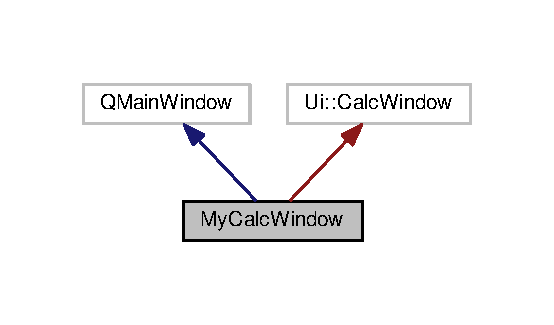
\includegraphics[width=266pt]{d9/d04/classMyCalcWindow__inherit__graph}
\end{center}
\end{figure}


Collaboration diagram for My\+Calc\+Window\+:
\nopagebreak
\begin{figure}[H]
\begin{center}
\leavevmode
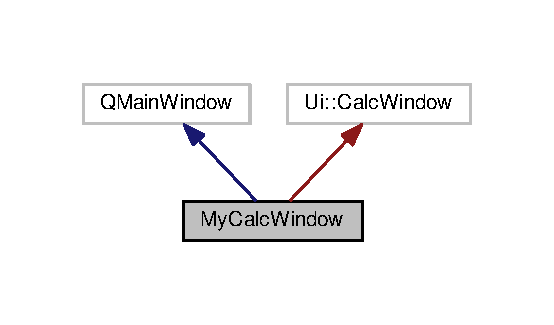
\includegraphics[width=322pt]{d6/dbc/classMyCalcWindow__coll__graph}
\end{center}
\end{figure}
\subsection*{Public Slots}
\begin{DoxyCompactItemize}
\item 
void \hyperlink{classMyCalcWindow_a6fdaf67619d3127503232c656e712656}{on\+\_\+exec\+Button\+\_\+clicked} (void)
\begin{DoxyCompactList}\small\item\em Slot chamado quando se clica no botão \textquotesingle{}Executar\textquotesingle{} e executa uma operação. \end{DoxyCompactList}\item 
void \hyperlink{classMyCalcWindow_ae1c714a5ad30c0fc67b9944481b30a05}{on\+\_\+radio\+Button\+Add\+\_\+clicked} (void)
\begin{DoxyCompactList}\small\item\em Slot chamado quando se clica no radio button da operação soma. \end{DoxyCompactList}\item 
void \hyperlink{classMyCalcWindow_a01fac328f5546feb830a67a7d35cc7f5}{on\+\_\+radio\+Button\+Sub\+\_\+clicked} (void)
\begin{DoxyCompactList}\small\item\em Slot chamado quando se clica no radio button da operação subtração. \end{DoxyCompactList}\item 
void \hyperlink{classMyCalcWindow_a553593de7766d99faf23a2053ddb4281}{on\+\_\+radio\+Button\+Mult\+\_\+clicked} (void)
\begin{DoxyCompactList}\small\item\em Slot chamado quando se clica no radio button da operação multiplicação. \end{DoxyCompactList}\item 
void \hyperlink{classMyCalcWindow_a1ac314ac5a743effc49465a295f796a4}{on\+\_\+radio\+Button\+Div\+\_\+clicked} (void)
\begin{DoxyCompactList}\small\item\em Slot chamado quando se clica no radio button da operação divisão. \end{DoxyCompactList}\item 
void \hyperlink{classMyCalcWindow_ad018832daea504f486bc1cb26f5cb0ec}{on\+\_\+action\+By\+User\+\_\+triggered} (void)
\begin{DoxyCompactList}\small\item\em Slot chamado quando selecionada a opção do menu \textquotesingle{}Por Usuário\textquotesingle{}. \end{DoxyCompactList}\item 
void \hyperlink{classMyCalcWindow_ab50a651bb1983993008960ad39d93ed6}{on\+\_\+action\+All\+Users\+\_\+triggered} (void)
\begin{DoxyCompactList}\small\item\em Slot chamado quando selecionada a opção do menu \textquotesingle{}Todos os Usuários\textquotesingle{}. \end{DoxyCompactList}\item 
void \hyperlink{classMyCalcWindow_ae563c8fa18e6d1c3a7c2c1014a133e66}{on\+\_\+user\+Role\+\_\+current\+Index\+Changed} (int)
\begin{DoxyCompactList}\small\item\em Método para delegar a atualização da interface dado uma mudança de papel do usuário. \end{DoxyCompactList}\item 
void \hyperlink{classMyCalcWindow_aa04caeaafdba97eeb25d3dd92be4d545}{on\+User\+Login} (\hyperlink{classUser}{User} $\ast$\hyperlink{classMyCalcWindow_a730189195d0831ae9fee62f7c519e439}{user})
\begin{DoxyCompactList}\small\item\em Slot chamado para se configurar a calculadora sobre informações de rede e usuário. \end{DoxyCompactList}\item 
void \hyperlink{classMyCalcWindow_a809b1da213d1424ba098c1f0ee2d0bd5}{on\+Quit} (void)\hypertarget{classMyCalcWindow_a809b1da213d1424ba098c1f0ee2d0bd5}{}\label{classMyCalcWindow_a809b1da213d1424ba098c1f0ee2d0bd5}

\begin{DoxyCompactList}\small\item\em Slot chamado ao se clicar no botão \textquotesingle{}Sair\textquotesingle{}. \end{DoxyCompactList}\item 
void \hyperlink{classMyCalcWindow_aaa868eba4e3ee5a52d28c0c34bbbd8cd}{read\+Message} (Q\+Json\+Object json\+Object)
\begin{DoxyCompactList}\small\item\em Slot chamado quando o socket recebe uma mensagem de resposta do servidor. \end{DoxyCompactList}\end{DoxyCompactItemize}
\subsection*{Public Member Functions}
\begin{DoxyCompactItemize}
\item 
\hyperlink{classMyCalcWindow_ac205ab2dbfbf802859774a090b066518}{My\+Calc\+Window} (Q\+Widget $\ast$parent=nullptr)
\begin{DoxyCompactList}\small\item\em Construtor Padrão para a classe \hyperlink{classMyCalcWindow}{My\+Calc\+Window}. \end{DoxyCompactList}\item 
virtual \hyperlink{classMyCalcWindow_a6226362b86860c067418d16b7da1e1e2}{$\sim$\+My\+Calc\+Window} ()
\begin{DoxyCompactList}\small\item\em Destrutor da classe \hyperlink{classMyCalcWindow}{My\+Calc\+Window}. \end{DoxyCompactList}\end{DoxyCompactItemize}
\subsection*{Private Member Functions}
\begin{DoxyCompactItemize}
\item 
void \hyperlink{classMyCalcWindow_a734b9dd51ee199d930855444695625c7}{execute} (void)
\begin{DoxyCompactList}\small\item\em Método privado para coleta dos dados e envio ao servidor para realização de operações. \end{DoxyCompactList}\item 
void \hyperlink{classMyCalcWindow_ade7d295cb55effe865349b7eef1a6d1a}{show\+Pie\+Chart} (Q\+String title, vector$<$ pair$<$ Q\+String, int $>$$>$ operations)
\begin{DoxyCompactList}\small\item\em Método é utilizado para se gerar exibições em gráfico pizza das operações realizadas, sejam por todos os usuários ou somente um deles. \end{DoxyCompactList}\item 
void \hyperlink{classMyCalcWindow_a9e1e6c80336ba383e2d2a8419446e1f9}{setup\+User\+Ui} (int role\+Code)
\begin{DoxyCompactList}\small\item\em Método para alterar a interface baseado no papel do usuário. \end{DoxyCompactList}\end{DoxyCompactItemize}
\subsection*{Private Attributes}
\begin{DoxyCompactItemize}
\item 
\hyperlink{classUser}{User} $\ast$ \hyperlink{classMyCalcWindow_a730189195d0831ae9fee62f7c519e439}{user}\hypertarget{classMyCalcWindow_a730189195d0831ae9fee62f7c519e439}{}\label{classMyCalcWindow_a730189195d0831ae9fee62f7c519e439}

\begin{DoxyCompactList}\small\item\em Referencia ao usuário da aplicação. \end{DoxyCompactList}\item 
Q\+Tcp\+Socket \hyperlink{classMyCalcWindow_aa07c81871dc4b11ab83324b544d66733}{tcp\+Socket}\hypertarget{classMyCalcWindow_aa07c81871dc4b11ab83324b544d66733}{}\label{classMyCalcWindow_aa07c81871dc4b11ab83324b544d66733}

\begin{DoxyCompactList}\small\item\em T\+C\+P\+Socket utilizado pela aplicação para comunicar com servidor. \end{DoxyCompactList}\item 
Q\+Main\+Window $\ast$ \hyperlink{classMyCalcWindow_a98ecf548e0cb3586ff4afc33bdfacb7a}{chart\+Window}\hypertarget{classMyCalcWindow_a98ecf548e0cb3586ff4afc33bdfacb7a}{}\label{classMyCalcWindow_a98ecf548e0cb3586ff4afc33bdfacb7a}

\begin{DoxyCompactList}\small\item\em Main\+Window auxiliar para exibição de gráficos de operações. \end{DoxyCompactList}\end{DoxyCompactItemize}
\subsection*{Static Private Attributes}
\begin{DoxyCompactItemize}
\item 
static const int \hyperlink{classMyCalcWindow_a5aad7da85f794398e01c5b553eff0fae}{U\+S\+ER} = 0\hypertarget{classMyCalcWindow_a5aad7da85f794398e01c5b553eff0fae}{}\label{classMyCalcWindow_a5aad7da85f794398e01c5b553eff0fae}

\begin{DoxyCompactList}\small\item\em Flag numerica representando o papel usuário. \end{DoxyCompactList}\item 
static const int \hyperlink{classMyCalcWindow_ac29d883c4ff53cc9d01c3e2add2fec52}{A\+D\+M\+IN} = 1\hypertarget{classMyCalcWindow_ac29d883c4ff53cc9d01c3e2add2fec52}{}\label{classMyCalcWindow_ac29d883c4ff53cc9d01c3e2add2fec52}

\begin{DoxyCompactList}\small\item\em Flag numerica representando o papel administrador. \end{DoxyCompactList}\end{DoxyCompactItemize}
\subsection*{Friends}
\begin{DoxyCompactItemize}
\item 
class \hyperlink{classMyCalcWindow_aec613ce0d143a48322f72a2b90819fcb}{My\+Login\+Dialog\+Test}\hypertarget{classMyCalcWindow_aec613ce0d143a48322f72a2b90819fcb}{}\label{classMyCalcWindow_aec613ce0d143a48322f72a2b90819fcb}

\begin{DoxyCompactList}\small\item\em Classe para Testes do \hyperlink{classMyLoginDialog}{My\+Login\+Dialog}. \end{DoxyCompactList}\item 
class \hyperlink{classMyCalcWindow_a5eaf2f81c93e423d3a80f10bd41e84f8}{My\+Calc\+Window\+Test}\hypertarget{classMyCalcWindow_a5eaf2f81c93e423d3a80f10bd41e84f8}{}\label{classMyCalcWindow_a5eaf2f81c93e423d3a80f10bd41e84f8}

\begin{DoxyCompactList}\small\item\em Classe para Testes do \hyperlink{classMyCalcWindow}{My\+Calc\+Window}. \end{DoxyCompactList}\end{DoxyCompactItemize}


\subsection{Detailed Description}
Classe para gerenciar as ações de uma calculadora. 

Esta classe gerencia as iterações do usuário com uma calculadora e delega todas suas operações a serem feitas no servidor. 

\subsection{Constructor \& Destructor Documentation}
\index{My\+Calc\+Window@{My\+Calc\+Window}!My\+Calc\+Window@{My\+Calc\+Window}}
\index{My\+Calc\+Window@{My\+Calc\+Window}!My\+Calc\+Window@{My\+Calc\+Window}}
\subsubsection[{\texorpdfstring{My\+Calc\+Window(\+Q\+Widget $\ast$parent=nullptr)}{MyCalcWindow(QWidget *parent=nullptr)}}]{\setlength{\rightskip}{0pt plus 5cm}My\+Calc\+Window\+::\+My\+Calc\+Window (
\begin{DoxyParamCaption}
\item[{Q\+Widget $\ast$}]{parent = {\ttfamily nullptr}}
\end{DoxyParamCaption}
)}\hypertarget{classMyCalcWindow_ac205ab2dbfbf802859774a090b066518}{}\label{classMyCalcWindow_ac205ab2dbfbf802859774a090b066518}


Construtor Padrão para a classe \hyperlink{classMyCalcWindow}{My\+Calc\+Window}. 

Esse construtor inicializa os atributos parent e chart\+Window. Além disso, o construtor configura a interface por meio do método \textquotesingle{}setup\+Ui\textquotesingle{} da classe pai Calc\+Window e conecta os slots para a leitura de mensagens do servidor e saída da aplicação.


\begin{DoxyParams}{Parameters}
{\em parent} & Referência ao componente pai. \\
\hline
\end{DoxyParams}
\index{My\+Calc\+Window@{My\+Calc\+Window}!````~My\+Calc\+Window@{$\sim$\+My\+Calc\+Window}}
\index{````~My\+Calc\+Window@{$\sim$\+My\+Calc\+Window}!My\+Calc\+Window@{My\+Calc\+Window}}
\subsubsection[{\texorpdfstring{$\sim$\+My\+Calc\+Window()}{~MyCalcWindow()}}]{\setlength{\rightskip}{0pt plus 5cm}My\+Calc\+Window\+::$\sim$\+My\+Calc\+Window (
\begin{DoxyParamCaption}
{}
\end{DoxyParamCaption}
)\hspace{0.3cm}{\ttfamily [virtual]}}\hypertarget{classMyCalcWindow_a6226362b86860c067418d16b7da1e1e2}{}\label{classMyCalcWindow_a6226362b86860c067418d16b7da1e1e2}


Destrutor da classe \hyperlink{classMyCalcWindow}{My\+Calc\+Window}. 

Esse destrutor é utilizado para deletar a referência contida em chart\+Window. 

\subsection{Member Function Documentation}
\index{My\+Calc\+Window@{My\+Calc\+Window}!execute@{execute}}
\index{execute@{execute}!My\+Calc\+Window@{My\+Calc\+Window}}
\subsubsection[{\texorpdfstring{execute(void)}{execute(void)}}]{\setlength{\rightskip}{0pt plus 5cm}void My\+Calc\+Window\+::execute (
\begin{DoxyParamCaption}
\item[{void}]{}
\end{DoxyParamCaption}
)\hspace{0.3cm}{\ttfamily [private]}}\hypertarget{classMyCalcWindow_a734b9dd51ee199d930855444695625c7}{}\label{classMyCalcWindow_a734b9dd51ee199d930855444695625c7}


Método privado para coleta dos dados e envio ao servidor para realização de operações. 

Este método extrai os dados da interface e solicita a execução da operação para o \hyperlink{classNetworkManager}{Network\+Manager}.

\begin{DoxySeeAlso}{See also}
\hyperlink{classMyCalcWindow_a6fdaf67619d3127503232c656e712656}{My\+Calc\+Window\+::on\+\_\+exec\+Button\+\_\+clicked()}, My\+Calc\+Window\+::on\+\_\+radio\+Button\+Soma\+\_\+clicked(), \hyperlink{classMyCalcWindow_a01fac328f5546feb830a67a7d35cc7f5}{My\+Calc\+Window\+::on\+\_\+radio\+Button\+Sub\+\_\+clicked()}, \hyperlink{classMyCalcWindow_a553593de7766d99faf23a2053ddb4281}{My\+Calc\+Window\+::on\+\_\+radio\+Button\+Mult\+\_\+clicked()}, \hyperlink{classMyCalcWindow_a1ac314ac5a743effc49465a295f796a4}{My\+Calc\+Window\+::on\+\_\+radio\+Button\+Div\+\_\+clicked()}, \hyperlink{classMyCalcWindow_aaa868eba4e3ee5a52d28c0c34bbbd8cd}{My\+Calc\+Window\+::read\+Message()}. 
\end{DoxySeeAlso}
\index{My\+Calc\+Window@{My\+Calc\+Window}!on\+\_\+action\+All\+Users\+\_\+triggered@{on\+\_\+action\+All\+Users\+\_\+triggered}}
\index{on\+\_\+action\+All\+Users\+\_\+triggered@{on\+\_\+action\+All\+Users\+\_\+triggered}!My\+Calc\+Window@{My\+Calc\+Window}}
\subsubsection[{\texorpdfstring{on\+\_\+action\+All\+Users\+\_\+triggered}{on_actionAllUsers_triggered}}]{\setlength{\rightskip}{0pt plus 5cm}void My\+Calc\+Window\+::on\+\_\+action\+All\+Users\+\_\+triggered (
\begin{DoxyParamCaption}
\item[{void}]{}
\end{DoxyParamCaption}
)\hspace{0.3cm}{\ttfamily [slot]}}\hypertarget{classMyCalcWindow_ab50a651bb1983993008960ad39d93ed6}{}\label{classMyCalcWindow_ab50a651bb1983993008960ad39d93ed6}


Slot chamado quando selecionada a opção do menu \textquotesingle{}Todos os Usuários\textquotesingle{}. 

Esse slot faz uma requisição ao \hyperlink{classNetworkManager}{Network\+Manager} dos dados de todas as operações realizadas por todos os usuários.

\begin{DoxySeeAlso}{See also}
\hyperlink{classMyCalcWindow_aaa868eba4e3ee5a52d28c0c34bbbd8cd}{My\+Calc\+Window\+::read\+Message()}, \hyperlink{classMyCalcWindow_ade7d295cb55effe865349b7eef1a6d1a}{My\+Calc\+Window\+::show\+Pie\+Chart(\+Q\+String, vector$<$pair$<$\+Q\+String, int$>$$>$)}. 
\end{DoxySeeAlso}
\index{My\+Calc\+Window@{My\+Calc\+Window}!on\+\_\+action\+By\+User\+\_\+triggered@{on\+\_\+action\+By\+User\+\_\+triggered}}
\index{on\+\_\+action\+By\+User\+\_\+triggered@{on\+\_\+action\+By\+User\+\_\+triggered}!My\+Calc\+Window@{My\+Calc\+Window}}
\subsubsection[{\texorpdfstring{on\+\_\+action\+By\+User\+\_\+triggered}{on_actionByUser_triggered}}]{\setlength{\rightskip}{0pt plus 5cm}void My\+Calc\+Window\+::on\+\_\+action\+By\+User\+\_\+triggered (
\begin{DoxyParamCaption}
\item[{void}]{}
\end{DoxyParamCaption}
)\hspace{0.3cm}{\ttfamily [slot]}}\hypertarget{classMyCalcWindow_ad018832daea504f486bc1cb26f5cb0ec}{}\label{classMyCalcWindow_ad018832daea504f486bc1cb26f5cb0ec}


Slot chamado quando selecionada a opção do menu \textquotesingle{}Por Usuário\textquotesingle{}. 

Esse slot faz uma requisição ao \hyperlink{classNetworkManager}{Network\+Manager} dos dados de todas as operações realizadas pelo usuário.

\begin{DoxySeeAlso}{See also}
\hyperlink{classMyCalcWindow_aaa868eba4e3ee5a52d28c0c34bbbd8cd}{My\+Calc\+Window\+::read\+Message()}, \hyperlink{classMyCalcWindow_ade7d295cb55effe865349b7eef1a6d1a}{My\+Calc\+Window\+::show\+Pie\+Chart(\+Q\+String, vector$<$pair$<$\+Q\+String, int$>$$>$)}. 
\end{DoxySeeAlso}
\index{My\+Calc\+Window@{My\+Calc\+Window}!on\+\_\+exec\+Button\+\_\+clicked@{on\+\_\+exec\+Button\+\_\+clicked}}
\index{on\+\_\+exec\+Button\+\_\+clicked@{on\+\_\+exec\+Button\+\_\+clicked}!My\+Calc\+Window@{My\+Calc\+Window}}
\subsubsection[{\texorpdfstring{on\+\_\+exec\+Button\+\_\+clicked}{on_execButton_clicked}}]{\setlength{\rightskip}{0pt plus 5cm}void My\+Calc\+Window\+::on\+\_\+exec\+Button\+\_\+clicked (
\begin{DoxyParamCaption}
\item[{void}]{}
\end{DoxyParamCaption}
)\hspace{0.3cm}{\ttfamily [slot]}}\hypertarget{classMyCalcWindow_a6fdaf67619d3127503232c656e712656}{}\label{classMyCalcWindow_a6fdaf67619d3127503232c656e712656}


Slot chamado quando se clica no botão \textquotesingle{}Executar\textquotesingle{} e executa uma operação. 

\begin{DoxySeeAlso}{See also}
\hyperlink{classMyCalcWindow_a734b9dd51ee199d930855444695625c7}{My\+Calc\+Window\+::execute()}. 
\end{DoxySeeAlso}
\index{My\+Calc\+Window@{My\+Calc\+Window}!on\+\_\+radio\+Button\+Add\+\_\+clicked@{on\+\_\+radio\+Button\+Add\+\_\+clicked}}
\index{on\+\_\+radio\+Button\+Add\+\_\+clicked@{on\+\_\+radio\+Button\+Add\+\_\+clicked}!My\+Calc\+Window@{My\+Calc\+Window}}
\subsubsection[{\texorpdfstring{on\+\_\+radio\+Button\+Add\+\_\+clicked}{on_radioButtonAdd_clicked}}]{\setlength{\rightskip}{0pt plus 5cm}void My\+Calc\+Window\+::on\+\_\+radio\+Button\+Add\+\_\+clicked (
\begin{DoxyParamCaption}
\item[{void}]{}
\end{DoxyParamCaption}
)\hspace{0.3cm}{\ttfamily [slot]}}\hypertarget{classMyCalcWindow_ae1c714a5ad30c0fc67b9944481b30a05}{}\label{classMyCalcWindow_ae1c714a5ad30c0fc67b9944481b30a05}


Slot chamado quando se clica no radio button da operação soma. 

\begin{DoxySeeAlso}{See also}
\hyperlink{classMyCalcWindow_a734b9dd51ee199d930855444695625c7}{My\+Calc\+Window\+::execute()}. 
\end{DoxySeeAlso}
\index{My\+Calc\+Window@{My\+Calc\+Window}!on\+\_\+radio\+Button\+Div\+\_\+clicked@{on\+\_\+radio\+Button\+Div\+\_\+clicked}}
\index{on\+\_\+radio\+Button\+Div\+\_\+clicked@{on\+\_\+radio\+Button\+Div\+\_\+clicked}!My\+Calc\+Window@{My\+Calc\+Window}}
\subsubsection[{\texorpdfstring{on\+\_\+radio\+Button\+Div\+\_\+clicked}{on_radioButtonDiv_clicked}}]{\setlength{\rightskip}{0pt plus 5cm}void My\+Calc\+Window\+::on\+\_\+radio\+Button\+Div\+\_\+clicked (
\begin{DoxyParamCaption}
\item[{void}]{}
\end{DoxyParamCaption}
)\hspace{0.3cm}{\ttfamily [slot]}}\hypertarget{classMyCalcWindow_a1ac314ac5a743effc49465a295f796a4}{}\label{classMyCalcWindow_a1ac314ac5a743effc49465a295f796a4}


Slot chamado quando se clica no radio button da operação divisão. 

\begin{DoxySeeAlso}{See also}
\hyperlink{classMyCalcWindow_a734b9dd51ee199d930855444695625c7}{My\+Calc\+Window\+::execute()}. 
\end{DoxySeeAlso}
\index{My\+Calc\+Window@{My\+Calc\+Window}!on\+\_\+radio\+Button\+Mult\+\_\+clicked@{on\+\_\+radio\+Button\+Mult\+\_\+clicked}}
\index{on\+\_\+radio\+Button\+Mult\+\_\+clicked@{on\+\_\+radio\+Button\+Mult\+\_\+clicked}!My\+Calc\+Window@{My\+Calc\+Window}}
\subsubsection[{\texorpdfstring{on\+\_\+radio\+Button\+Mult\+\_\+clicked}{on_radioButtonMult_clicked}}]{\setlength{\rightskip}{0pt plus 5cm}void My\+Calc\+Window\+::on\+\_\+radio\+Button\+Mult\+\_\+clicked (
\begin{DoxyParamCaption}
\item[{void}]{}
\end{DoxyParamCaption}
)\hspace{0.3cm}{\ttfamily [slot]}}\hypertarget{classMyCalcWindow_a553593de7766d99faf23a2053ddb4281}{}\label{classMyCalcWindow_a553593de7766d99faf23a2053ddb4281}


Slot chamado quando se clica no radio button da operação multiplicação. 

\begin{DoxySeeAlso}{See also}
\hyperlink{classMyCalcWindow_a734b9dd51ee199d930855444695625c7}{My\+Calc\+Window\+::execute()}. 
\end{DoxySeeAlso}
\index{My\+Calc\+Window@{My\+Calc\+Window}!on\+\_\+radio\+Button\+Sub\+\_\+clicked@{on\+\_\+radio\+Button\+Sub\+\_\+clicked}}
\index{on\+\_\+radio\+Button\+Sub\+\_\+clicked@{on\+\_\+radio\+Button\+Sub\+\_\+clicked}!My\+Calc\+Window@{My\+Calc\+Window}}
\subsubsection[{\texorpdfstring{on\+\_\+radio\+Button\+Sub\+\_\+clicked}{on_radioButtonSub_clicked}}]{\setlength{\rightskip}{0pt plus 5cm}void My\+Calc\+Window\+::on\+\_\+radio\+Button\+Sub\+\_\+clicked (
\begin{DoxyParamCaption}
\item[{void}]{}
\end{DoxyParamCaption}
)\hspace{0.3cm}{\ttfamily [slot]}}\hypertarget{classMyCalcWindow_a01fac328f5546feb830a67a7d35cc7f5}{}\label{classMyCalcWindow_a01fac328f5546feb830a67a7d35cc7f5}


Slot chamado quando se clica no radio button da operação subtração. 

\begin{DoxySeeAlso}{See also}
\hyperlink{classMyCalcWindow_a734b9dd51ee199d930855444695625c7}{My\+Calc\+Window\+::execute()}. 
\end{DoxySeeAlso}
\index{My\+Calc\+Window@{My\+Calc\+Window}!on\+\_\+user\+Role\+\_\+current\+Index\+Changed@{on\+\_\+user\+Role\+\_\+current\+Index\+Changed}}
\index{on\+\_\+user\+Role\+\_\+current\+Index\+Changed@{on\+\_\+user\+Role\+\_\+current\+Index\+Changed}!My\+Calc\+Window@{My\+Calc\+Window}}
\subsubsection[{\texorpdfstring{on\+\_\+user\+Role\+\_\+current\+Index\+Changed}{on_userRole_currentIndexChanged}}]{\setlength{\rightskip}{0pt plus 5cm}void My\+Calc\+Window\+::on\+\_\+user\+Role\+\_\+current\+Index\+Changed (
\begin{DoxyParamCaption}
\item[{int}]{position}
\end{DoxyParamCaption}
)\hspace{0.3cm}{\ttfamily [slot]}}\hypertarget{classMyCalcWindow_ae563c8fa18e6d1c3a7c2c1014a133e66}{}\label{classMyCalcWindow_ae563c8fa18e6d1c3a7c2c1014a133e66}


Método para delegar a atualização da interface dado uma mudança de papel do usuário. 


\begin{DoxyParams}{Parameters}
{\em position} & Opção selecionada no combo box \\
\hline
\end{DoxyParams}
\index{My\+Calc\+Window@{My\+Calc\+Window}!on\+User\+Login@{on\+User\+Login}}
\index{on\+User\+Login@{on\+User\+Login}!My\+Calc\+Window@{My\+Calc\+Window}}
\subsubsection[{\texorpdfstring{on\+User\+Login}{onUserLogin}}]{\setlength{\rightskip}{0pt plus 5cm}void My\+Calc\+Window\+::on\+User\+Login (
\begin{DoxyParamCaption}
\item[{{\bf User} $\ast$}]{user}
\end{DoxyParamCaption}
)\hspace{0.3cm}{\ttfamily [slot]}}\hypertarget{classMyCalcWindow_aa04caeaafdba97eeb25d3dd92be4d545}{}\label{classMyCalcWindow_aa04caeaafdba97eeb25d3dd92be4d545}


Slot chamado para se configurar a calculadora sobre informações de rede e usuário. 


\begin{DoxyParams}{Parameters}
{\em user} & Referencia ao usuário da aplicação. \\
\hline
\end{DoxyParams}
\index{My\+Calc\+Window@{My\+Calc\+Window}!read\+Message@{read\+Message}}
\index{read\+Message@{read\+Message}!My\+Calc\+Window@{My\+Calc\+Window}}
\subsubsection[{\texorpdfstring{read\+Message}{readMessage}}]{\setlength{\rightskip}{0pt plus 5cm}void My\+Calc\+Window\+::read\+Message (
\begin{DoxyParamCaption}
\item[{Q\+Json\+Object}]{json\+Object}
\end{DoxyParamCaption}
)\hspace{0.3cm}{\ttfamily [slot]}}\hypertarget{classMyCalcWindow_aaa868eba4e3ee5a52d28c0c34bbbd8cd}{}\label{classMyCalcWindow_aaa868eba4e3ee5a52d28c0c34bbbd8cd}


Slot chamado quando o socket recebe uma mensagem de resposta do servidor. 

Ao receber uma resposta do \hyperlink{classNetworkManager}{Network\+Manager}, este método extrai as informações da mensagem e realiza a operação correspondente.

\begin{DoxySeeAlso}{See also}
\hyperlink{classMyCalcWindow_a734b9dd51ee199d930855444695625c7}{My\+Calc\+Window\+::execute()}, \hyperlink{classMyCalcWindow_ab50a651bb1983993008960ad39d93ed6}{My\+Calc\+Window\+::on\+\_\+action\+All\+Users\+\_\+triggered()}, \hyperlink{classMyCalcWindow_ad018832daea504f486bc1cb26f5cb0ec}{My\+Calc\+Window\+::on\+\_\+action\+By\+User\+\_\+triggered()}. 
\end{DoxySeeAlso}
\index{My\+Calc\+Window@{My\+Calc\+Window}!setup\+User\+Ui@{setup\+User\+Ui}}
\index{setup\+User\+Ui@{setup\+User\+Ui}!My\+Calc\+Window@{My\+Calc\+Window}}
\subsubsection[{\texorpdfstring{setup\+User\+Ui(int role\+Code)}{setupUserUi(int roleCode)}}]{\setlength{\rightskip}{0pt plus 5cm}void My\+Calc\+Window\+::setup\+User\+Ui (
\begin{DoxyParamCaption}
\item[{int}]{role\+Code}
\end{DoxyParamCaption}
)\hspace{0.3cm}{\ttfamily [private]}}\hypertarget{classMyCalcWindow_a9e1e6c80336ba383e2d2a8419446e1f9}{}\label{classMyCalcWindow_a9e1e6c80336ba383e2d2a8419446e1f9}


Método para alterar a interface baseado no papel do usuário. 


\begin{DoxyParams}{Parameters}
{\em role\+Code} & código do papel do usuário \\
\hline
\end{DoxyParams}
\index{My\+Calc\+Window@{My\+Calc\+Window}!show\+Pie\+Chart@{show\+Pie\+Chart}}
\index{show\+Pie\+Chart@{show\+Pie\+Chart}!My\+Calc\+Window@{My\+Calc\+Window}}
\subsubsection[{\texorpdfstring{show\+Pie\+Chart(\+Q\+String title, vector$<$ pair$<$ Q\+String, int $>$$>$ operations)}{showPieChart(QString title, vector< pair< QString, int >> operations)}}]{\setlength{\rightskip}{0pt plus 5cm}void My\+Calc\+Window\+::show\+Pie\+Chart (
\begin{DoxyParamCaption}
\item[{Q\+String}]{title, }
\item[{vector$<$ pair$<$ Q\+String, int $>$$>$}]{operations}
\end{DoxyParamCaption}
)\hspace{0.3cm}{\ttfamily [private]}}\hypertarget{classMyCalcWindow_ade7d295cb55effe865349b7eef1a6d1a}{}\label{classMyCalcWindow_ade7d295cb55effe865349b7eef1a6d1a}


Método é utilizado para se gerar exibições em gráfico pizza das operações realizadas, sejam por todos os usuários ou somente um deles. 


\begin{DoxyParams}{Parameters}
{\em title} & Título do gráfico. \\
\hline
{\em operations} & Vetor contendo os dados das operações em pares (Operação, Quantidade).\\
\hline
\end{DoxyParams}
\begin{DoxySeeAlso}{See also}
\hyperlink{classMyCalcWindow_ad018832daea504f486bc1cb26f5cb0ec}{My\+Calc\+Window\+::on\+\_\+action\+By\+User\+\_\+triggered()}, My\+Calc\+Window\+::on\+\_\+action\+All\+User\+\_\+triggered(). 
\end{DoxySeeAlso}


The documentation for this class was generated from the following files\+:\begin{DoxyCompactItemize}
\item 
Calc\+Client/src/gui/\hyperlink{mycalcwindow_8h}{mycalcwindow.\+h}\item 
Calc\+Client/src/gui/\hyperlink{mycalcwindow_8cpp}{mycalcwindow.\+cpp}\end{DoxyCompactItemize}

\hypertarget{classMyLoginDialog}{}\section{My\+Login\+Dialog Class Reference}
\label{classMyLoginDialog}\index{My\+Login\+Dialog@{My\+Login\+Dialog}}


Classe para gerenciar as requisições de login.  




{\ttfamily \#include $<$mylogindialog.\+h$>$}



Inheritance diagram for My\+Login\+Dialog\+:
\nopagebreak
\begin{figure}[H]
\begin{center}
\leavevmode
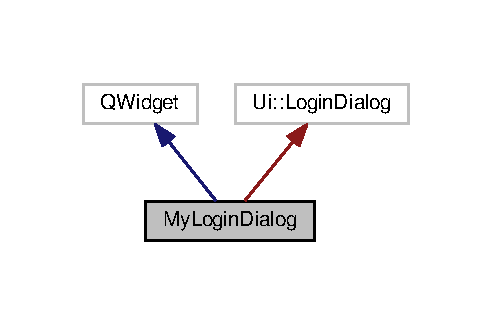
\includegraphics[width=236pt]{d5/d81/classMyLoginDialog__inherit__graph}
\end{center}
\end{figure}


Collaboration diagram for My\+Login\+Dialog\+:
\nopagebreak
\begin{figure}[H]
\begin{center}
\leavevmode
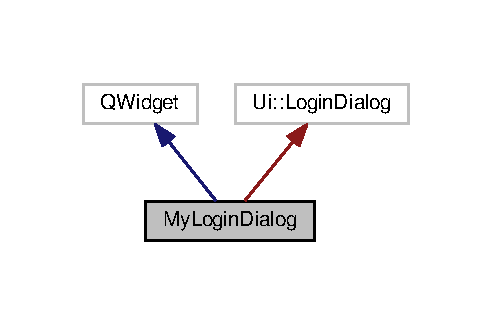
\includegraphics[width=236pt]{db/d47/classMyLoginDialog__coll__graph}
\end{center}
\end{figure}
\subsection*{Public Slots}
\begin{DoxyCompactItemize}
\item 
void \hyperlink{classMyLoginDialog_ab850edc55bc360a5271f8da572d9b84b}{on\+\_\+login\+\_\+button\+\_\+clicked} (void)
\begin{DoxyCompactList}\small\item\em Slot chamado para realizar a operação de login. \end{DoxyCompactList}\item 
void \hyperlink{classMyLoginDialog_a98b534e1f3e50217b7d0d603846f6fa3}{on\+\_\+cancel\+\_\+button\+\_\+clicked} (void)
\begin{DoxyCompactList}\small\item\em Slot chamado para finalizar a aplicação. \end{DoxyCompactList}\item 
void \hyperlink{classMyLoginDialog_a6def7158f19720b26ac23274b38ddc2d}{read\+Message} (Q\+Json\+Object json\+Object)
\begin{DoxyCompactList}\small\item\em Slot chamado quando o socket recebe uma mensagem de resposta do servidor. \end{DoxyCompactList}\end{DoxyCompactItemize}
\subsection*{Signals}
\begin{DoxyCompactItemize}
\item 
void \hyperlink{classMyLoginDialog_af34aa4fb816da6adb7813ced2779cc3e}{logged} (Q\+String username, bool admin\+Level)
\begin{DoxyCompactList}\small\item\em Signal emitido quando a operação de login é realizada com sucesso. \end{DoxyCompactList}\item 
void \hyperlink{classMyLoginDialog_a81b2fde13842c6557400e0e35b9dd1e0}{quit} (void)\hypertarget{classMyLoginDialog_a81b2fde13842c6557400e0e35b9dd1e0}{}\label{classMyLoginDialog_a81b2fde13842c6557400e0e35b9dd1e0}

\begin{DoxyCompactList}\small\item\em Signal emitido para finalizar a aplicação. \end{DoxyCompactList}\end{DoxyCompactItemize}
\subsection*{Public Member Functions}
\begin{DoxyCompactItemize}
\item 
\hyperlink{classMyLoginDialog_ae20170dfe9e23fc1b794d3b5a2d2cc97}{My\+Login\+Dialog} (Q\+Widget $\ast$parent=nullptr)
\begin{DoxyCompactList}\small\item\em Construtor Padrão para a classe \hyperlink{classMyLoginDialog}{My\+Login\+Dialog}. \end{DoxyCompactList}\end{DoxyCompactItemize}
\subsection*{Private Attributes}
\begin{DoxyCompactItemize}
\item 
Q\+Tcp\+Socket \hyperlink{classMyLoginDialog_aea07f561f3a3e17b6596da377a538e4f}{tcp\+Socket}\hypertarget{classMyLoginDialog_aea07f561f3a3e17b6596da377a538e4f}{}\label{classMyLoginDialog_aea07f561f3a3e17b6596da377a538e4f}

\begin{DoxyCompactList}\small\item\em T\+C\+P\+Socket utilizado pela aplicação para comunicar com servidor. \end{DoxyCompactList}\end{DoxyCompactItemize}
\subsection*{Friends}
\begin{DoxyCompactItemize}
\item 
class \hyperlink{classMyLoginDialog_aec613ce0d143a48322f72a2b90819fcb}{My\+Login\+Dialog\+Test}\hypertarget{classMyLoginDialog_aec613ce0d143a48322f72a2b90819fcb}{}\label{classMyLoginDialog_aec613ce0d143a48322f72a2b90819fcb}

\begin{DoxyCompactList}\small\item\em Classe para Testes de \hyperlink{classMyLoginDialog}{My\+Login\+Dialog}. \end{DoxyCompactList}\end{DoxyCompactItemize}


\subsection{Detailed Description}
Classe para gerenciar as requisições de login. 

Esta classe gerencia as iterações do usuário com uma janela de login e realiza a validação dos dados em um servidor. 

\subsection{Constructor \& Destructor Documentation}
\index{My\+Login\+Dialog@{My\+Login\+Dialog}!My\+Login\+Dialog@{My\+Login\+Dialog}}
\index{My\+Login\+Dialog@{My\+Login\+Dialog}!My\+Login\+Dialog@{My\+Login\+Dialog}}
\subsubsection[{\texorpdfstring{My\+Login\+Dialog(\+Q\+Widget $\ast$parent=nullptr)}{MyLoginDialog(QWidget *parent=nullptr)}}]{\setlength{\rightskip}{0pt plus 5cm}My\+Login\+Dialog\+::\+My\+Login\+Dialog (
\begin{DoxyParamCaption}
\item[{Q\+Widget $\ast$}]{parent = {\ttfamily nullptr}}
\end{DoxyParamCaption}
)}\hypertarget{classMyLoginDialog_ae20170dfe9e23fc1b794d3b5a2d2cc97}{}\label{classMyLoginDialog_ae20170dfe9e23fc1b794d3b5a2d2cc97}


Construtor Padrão para a classe \hyperlink{classMyLoginDialog}{My\+Login\+Dialog}. 

Inicializa o atributo parent, configura a interface por meio do método \textquotesingle{}setup\+Ui\textquotesingle{} da classe pai Login\+Dialog e conecta o slot para a leitura de mensagens do servidor.


\begin{DoxyParams}{Parameters}
{\em parent} & Referência ao componente pai. \\
\hline
\end{DoxyParams}


\subsection{Member Function Documentation}
\index{My\+Login\+Dialog@{My\+Login\+Dialog}!logged@{logged}}
\index{logged@{logged}!My\+Login\+Dialog@{My\+Login\+Dialog}}
\subsubsection[{\texorpdfstring{logged}{logged}}]{\setlength{\rightskip}{0pt plus 5cm}void My\+Login\+Dialog\+::logged (
\begin{DoxyParamCaption}
\item[{Q\+String}]{username, }
\item[{bool}]{admin\+Level}
\end{DoxyParamCaption}
)\hspace{0.3cm}{\ttfamily [signal]}}\hypertarget{classMyLoginDialog_af34aa4fb816da6adb7813ced2779cc3e}{}\label{classMyLoginDialog_af34aa4fb816da6adb7813ced2779cc3e}


Signal emitido quando a operação de login é realizada com sucesso. 


\begin{DoxyParams}{Parameters}
{\em username} & Nome do usuário. \\
\hline
{\em admin\+Level} & Flag identificando se o usuário é administrador. \\
\hline
\end{DoxyParams}
\index{My\+Login\+Dialog@{My\+Login\+Dialog}!on\+\_\+cancel\+\_\+button\+\_\+clicked@{on\+\_\+cancel\+\_\+button\+\_\+clicked}}
\index{on\+\_\+cancel\+\_\+button\+\_\+clicked@{on\+\_\+cancel\+\_\+button\+\_\+clicked}!My\+Login\+Dialog@{My\+Login\+Dialog}}
\subsubsection[{\texorpdfstring{on\+\_\+cancel\+\_\+button\+\_\+clicked}{on_cancel_button_clicked}}]{\setlength{\rightskip}{0pt plus 5cm}void My\+Login\+Dialog\+::on\+\_\+cancel\+\_\+button\+\_\+clicked (
\begin{DoxyParamCaption}
\item[{void}]{}
\end{DoxyParamCaption}
)\hspace{0.3cm}{\ttfamily [slot]}}\hypertarget{classMyLoginDialog_a98b534e1f3e50217b7d0d603846f6fa3}{}\label{classMyLoginDialog_a98b534e1f3e50217b7d0d603846f6fa3}


Slot chamado para finalizar a aplicação. 

\begin{DoxySeeAlso}{See also}
\hyperlink{classMyLoginDialog_a81b2fde13842c6557400e0e35b9dd1e0}{My\+Login\+Dialog\+::quit()}. 
\end{DoxySeeAlso}
\index{My\+Login\+Dialog@{My\+Login\+Dialog}!on\+\_\+login\+\_\+button\+\_\+clicked@{on\+\_\+login\+\_\+button\+\_\+clicked}}
\index{on\+\_\+login\+\_\+button\+\_\+clicked@{on\+\_\+login\+\_\+button\+\_\+clicked}!My\+Login\+Dialog@{My\+Login\+Dialog}}
\subsubsection[{\texorpdfstring{on\+\_\+login\+\_\+button\+\_\+clicked}{on_login_button_clicked}}]{\setlength{\rightskip}{0pt plus 5cm}void My\+Login\+Dialog\+::on\+\_\+login\+\_\+button\+\_\+clicked (
\begin{DoxyParamCaption}
\item[{void}]{}
\end{DoxyParamCaption}
)\hspace{0.3cm}{\ttfamily [slot]}}\hypertarget{classMyLoginDialog_ab850edc55bc360a5271f8da572d9b84b}{}\label{classMyLoginDialog_ab850edc55bc360a5271f8da572d9b84b}


Slot chamado para realizar a operação de login. 

Recupera as informações da interface e realiza um requisição de autenticação ao servidor.

\begin{DoxySeeAlso}{See also}
\hyperlink{classMyLoginDialog_a6def7158f19720b26ac23274b38ddc2d}{My\+Login\+Dialog\+::read\+Message()}. 
\end{DoxySeeAlso}
\index{My\+Login\+Dialog@{My\+Login\+Dialog}!read\+Message@{read\+Message}}
\index{read\+Message@{read\+Message}!My\+Login\+Dialog@{My\+Login\+Dialog}}
\subsubsection[{\texorpdfstring{read\+Message}{readMessage}}]{\setlength{\rightskip}{0pt plus 5cm}void My\+Login\+Dialog\+::read\+Message (
\begin{DoxyParamCaption}
\item[{Q\+Json\+Object}]{json\+Object}
\end{DoxyParamCaption}
)\hspace{0.3cm}{\ttfamily [slot]}}\hypertarget{classMyLoginDialog_a6def7158f19720b26ac23274b38ddc2d}{}\label{classMyLoginDialog_a6def7158f19720b26ac23274b38ddc2d}


Slot chamado quando o socket recebe uma mensagem de resposta do servidor. 

Esse método recebe uma resposta do servidor sobre a tentativa de login. Caso positivo emite um signal informando que o usuário foi autenticado. Caso contrário mostra uma janela de erro.

\begin{DoxySeeAlso}{See also}
\hyperlink{classMyLoginDialog_ab850edc55bc360a5271f8da572d9b84b}{My\+Login\+Dialog\+::on\+\_\+login\+\_\+button\+\_\+clicked()}, My\+Login\+Dialog\+::logged(\+Q\+String,bool,\+Q\+String,int). 
\end{DoxySeeAlso}


The documentation for this class was generated from the following files\+:\begin{DoxyCompactItemize}
\item 
Calc\+Client/src/gui/\hyperlink{mylogindialog_8h}{mylogindialog.\+h}\item 
Calc\+Client/src/gui/\hyperlink{mylogindialog_8cpp}{mylogindialog.\+cpp}\end{DoxyCompactItemize}

\hypertarget{classNetworkManager}{}\section{Network\+Manager Class Reference}
\label{classNetworkManager}\index{Network\+Manager@{Network\+Manager}}


Classe para gerenciar comunicações entre a gui e o server pela rede.  




{\ttfamily \#include $<$networkmanager.\+h$>$}



Inheritance diagram for Network\+Manager\+:
\nopagebreak
\begin{figure}[H]
\begin{center}
\leavevmode
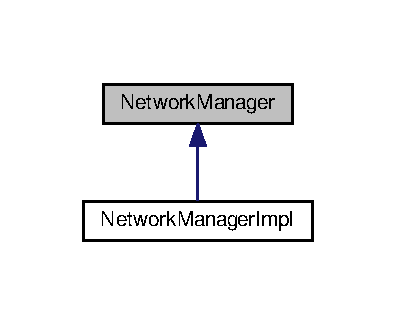
\includegraphics[width=190pt]{d5/da1/classNetworkManager__inherit__graph}
\end{center}
\end{figure}


Collaboration diagram for Network\+Manager\+:
\nopagebreak
\begin{figure}[H]
\begin{center}
\leavevmode
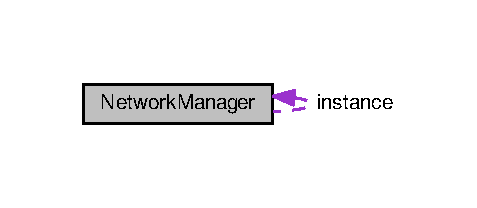
\includegraphics[width=229pt]{d5/d38/classNetworkManager__coll__graph}
\end{center}
\end{figure}
\subsection*{Public Member Functions}
\begin{DoxyCompactItemize}
\item 
virtual void \hyperlink{classNetworkManager_ae7b073b1deb224a6cb7af0e4d3d158de}{configure} (Q\+String ip, quint16 port)=0
\begin{DoxyCompactList}\small\item\em Método para configurar o \hyperlink{classNetworkManager}{Network\+Manager}. \end{DoxyCompactList}\item 
virtual void \hyperlink{classNetworkManager_ae0f54c8b721ad7ab34e4ce414e23f90f}{login} (\hyperlink{classBasicUser}{Basic\+User} $\ast$basic\+User)=0
\begin{DoxyCompactList}\small\item\em Método para realizar um login. \end{DoxyCompactList}\item 
virtual void \hyperlink{classNetworkManager_acf9c749d6bd57e7e1e4f542a33657425}{do\+Operation} (\hyperlink{classBasicUser}{Basic\+User} $\ast$basic\+User, double factor1, double factor2, int op\+Code)=0
\begin{DoxyCompactList}\small\item\em Método para realizar operações matematicas. \end{DoxyCompactList}\item 
virtual void \hyperlink{classNetworkManager_a2a1c3b3d0bc298a621820e723e3141af}{report\+By\+User} (\hyperlink{classBasicUser}{Basic\+User} $\ast$basic\+User)=0
\begin{DoxyCompactList}\small\item\em Método para recuperar o relatorio de operações do usuário. \end{DoxyCompactList}\item 
virtual void \hyperlink{classNetworkManager_adc90f12e3f926a79382aefbceb3aecfc}{report\+All\+Users} (\hyperlink{classAdminUser}{Admin\+User} $\ast$admin\+User)=0
\begin{DoxyCompactList}\small\item\em Método para recuperar o relatorio de operações de todos os usuários. \end{DoxyCompactList}\item 
virtual Q\+Object $\ast$ \hyperlink{classNetworkManager_a437755d5e84ea8522515283ba11f4b77}{get\+Q\+Object} ()=0
\begin{DoxyCompactList}\small\item\em Retorna um Q\+Object referente a \hyperlink{classNetworkManager}{Network\+Manager}. \end{DoxyCompactList}\item 
virtual void \hyperlink{classNetworkManager_a5200afa56c88ff5d5779a39fec1ab33c}{message\+Receive} (Q\+Json\+Object json\+Object)=0
\begin{DoxyCompactList}\small\item\em Método que recebe como parametro o Json correspondente da resposta. \end{DoxyCompactList}\end{DoxyCompactItemize}
\subsection*{Static Public Member Functions}
\begin{DoxyCompactItemize}
\item 
static \hyperlink{classNetworkManager}{Network\+Manager} $\ast$ \hyperlink{classNetworkManager_a160c056e7177dbe9686310e4896326d6}{get\+Instance} ()
\begin{DoxyCompactList}\small\item\em Este método retorna uma instancia de \hyperlink{classNetworkManager}{Network\+Manager}. \end{DoxyCompactList}\end{DoxyCompactItemize}
\subsection*{Static Private Attributes}
\begin{DoxyCompactItemize}
\item 
static \hyperlink{classNetworkManager}{Network\+Manager} $\ast$ \hyperlink{classNetworkManager_a1bf872fb0f00ebc5ed6fecd2016874e2}{instance} = nullptr\hypertarget{classNetworkManager_a1bf872fb0f00ebc5ed6fecd2016874e2}{}\label{classNetworkManager_a1bf872fb0f00ebc5ed6fecd2016874e2}

\begin{DoxyCompactList}\small\item\em Instancia única da classe. \end{DoxyCompactList}\end{DoxyCompactItemize}


\subsection{Detailed Description}
Classe para gerenciar comunicações entre a gui e o server pela rede. 

\subsection{Member Function Documentation}
\index{Network\+Manager@{Network\+Manager}!configure@{configure}}
\index{configure@{configure}!Network\+Manager@{Network\+Manager}}
\subsubsection[{\texorpdfstring{configure(\+Q\+String ip, quint16 port)=0}{configure(QString ip, quint16 port)=0}}]{\setlength{\rightskip}{0pt plus 5cm}virtual void Network\+Manager\+::configure (
\begin{DoxyParamCaption}
\item[{Q\+String}]{ip, }
\item[{quint16}]{port}
\end{DoxyParamCaption}
)\hspace{0.3cm}{\ttfamily [pure virtual]}}\hypertarget{classNetworkManager_ae7b073b1deb224a6cb7af0e4d3d158de}{}\label{classNetworkManager_ae7b073b1deb224a6cb7af0e4d3d158de}


Método para configurar o \hyperlink{classNetworkManager}{Network\+Manager}. 


\begin{DoxyParams}{Parameters}
{\em ip} & Ip do Servidor \\
\hline
{\em port} & Porta do Servidor \\
\hline
\end{DoxyParams}


Implemented in \hyperlink{classNetworkManagerImpl_a4ad2bada544bc02ea1f9921f3f6f62c2}{Network\+Manager\+Impl}.

\index{Network\+Manager@{Network\+Manager}!do\+Operation@{do\+Operation}}
\index{do\+Operation@{do\+Operation}!Network\+Manager@{Network\+Manager}}
\subsubsection[{\texorpdfstring{do\+Operation(\+Basic\+User $\ast$basic\+User, double factor1, double factor2, int op\+Code)=0}{doOperation(BasicUser *basicUser, double factor1, double factor2, int opCode)=0}}]{\setlength{\rightskip}{0pt plus 5cm}virtual void Network\+Manager\+::do\+Operation (
\begin{DoxyParamCaption}
\item[{{\bf Basic\+User} $\ast$}]{basic\+User, }
\item[{double}]{factor1, }
\item[{double}]{factor2, }
\item[{int}]{op\+Code}
\end{DoxyParamCaption}
)\hspace{0.3cm}{\ttfamily [pure virtual]}}\hypertarget{classNetworkManager_acf9c749d6bd57e7e1e4f542a33657425}{}\label{classNetworkManager_acf9c749d6bd57e7e1e4f542a33657425}


Método para realizar operações matematicas. 


\begin{DoxyParams}{Parameters}
{\em basic\+User} & Objeto representando um usuário basico do sistema \\
\hline
{\em factor1} & Primeiro fator da operação \\
\hline
{\em factor2} & Segundo fator da operação \\
\hline
{\em op\+Code} & Código da operação \\
\hline
\end{DoxyParams}


Implemented in \hyperlink{classNetworkManagerImpl_a890d3968345656de525f042dbc281507}{Network\+Manager\+Impl}.

\index{Network\+Manager@{Network\+Manager}!get\+Instance@{get\+Instance}}
\index{get\+Instance@{get\+Instance}!Network\+Manager@{Network\+Manager}}
\subsubsection[{\texorpdfstring{get\+Instance()}{getInstance()}}]{\setlength{\rightskip}{0pt plus 5cm}{\bf Network\+Manager} $\ast$ Network\+Manager\+::get\+Instance (
\begin{DoxyParamCaption}
{}
\end{DoxyParamCaption}
)\hspace{0.3cm}{\ttfamily [static]}}\hypertarget{classNetworkManager_a160c056e7177dbe9686310e4896326d6}{}\label{classNetworkManager_a160c056e7177dbe9686310e4896326d6}


Este método retorna uma instancia de \hyperlink{classNetworkManager}{Network\+Manager}. 

\begin{DoxyReturn}{Returns}
Instancia de Network\+Manager$\ast$ 
\end{DoxyReturn}
\index{Network\+Manager@{Network\+Manager}!get\+Q\+Object@{get\+Q\+Object}}
\index{get\+Q\+Object@{get\+Q\+Object}!Network\+Manager@{Network\+Manager}}
\subsubsection[{\texorpdfstring{get\+Q\+Object()=0}{getQObject()=0}}]{\setlength{\rightskip}{0pt plus 5cm}virtual Q\+Object$\ast$ Network\+Manager\+::get\+Q\+Object (
\begin{DoxyParamCaption}
{}
\end{DoxyParamCaption}
)\hspace{0.3cm}{\ttfamily [pure virtual]}}\hypertarget{classNetworkManager_a437755d5e84ea8522515283ba11f4b77}{}\label{classNetworkManager_a437755d5e84ea8522515283ba11f4b77}


Retorna um Q\+Object referente a \hyperlink{classNetworkManager}{Network\+Manager}. 

\begin{DoxyReturn}{Returns}
Q\+Object correspondente 
\end{DoxyReturn}


Implemented in \hyperlink{classNetworkManagerImpl_a3340057281dadf1861d94d8aba9e976e}{Network\+Manager\+Impl}.

\index{Network\+Manager@{Network\+Manager}!login@{login}}
\index{login@{login}!Network\+Manager@{Network\+Manager}}
\subsubsection[{\texorpdfstring{login(\+Basic\+User $\ast$basic\+User)=0}{login(BasicUser *basicUser)=0}}]{\setlength{\rightskip}{0pt plus 5cm}virtual void Network\+Manager\+::login (
\begin{DoxyParamCaption}
\item[{{\bf Basic\+User} $\ast$}]{basic\+User}
\end{DoxyParamCaption}
)\hspace{0.3cm}{\ttfamily [pure virtual]}}\hypertarget{classNetworkManager_ae0f54c8b721ad7ab34e4ce414e23f90f}{}\label{classNetworkManager_ae0f54c8b721ad7ab34e4ce414e23f90f}


Método para realizar um login. 


\begin{DoxyParams}{Parameters}
{\em basic\+User} & Objeto representando um usuário basico do sistema \\
\hline
\end{DoxyParams}


Implemented in \hyperlink{classNetworkManagerImpl_a59dfa1a94c491fadbd62197a36c806b6}{Network\+Manager\+Impl}.

\index{Network\+Manager@{Network\+Manager}!message\+Receive@{message\+Receive}}
\index{message\+Receive@{message\+Receive}!Network\+Manager@{Network\+Manager}}
\subsubsection[{\texorpdfstring{message\+Receive(\+Q\+Json\+Object json\+Object)=0}{messageReceive(QJsonObject jsonObject)=0}}]{\setlength{\rightskip}{0pt plus 5cm}virtual void Network\+Manager\+::message\+Receive (
\begin{DoxyParamCaption}
\item[{Q\+Json\+Object}]{json\+Object}
\end{DoxyParamCaption}
)\hspace{0.3cm}{\ttfamily [pure virtual]}}\hypertarget{classNetworkManager_a5200afa56c88ff5d5779a39fec1ab33c}{}\label{classNetworkManager_a5200afa56c88ff5d5779a39fec1ab33c}


Método que recebe como parametro o Json correspondente da resposta. 


\begin{DoxyParams}{Parameters}
{\em json\+Object} & Resposta recebida do servidor \\
\hline
\end{DoxyParams}
\index{Network\+Manager@{Network\+Manager}!report\+All\+Users@{report\+All\+Users}}
\index{report\+All\+Users@{report\+All\+Users}!Network\+Manager@{Network\+Manager}}
\subsubsection[{\texorpdfstring{report\+All\+Users(\+Admin\+User $\ast$admin\+User)=0}{reportAllUsers(AdminUser *adminUser)=0}}]{\setlength{\rightskip}{0pt plus 5cm}virtual void Network\+Manager\+::report\+All\+Users (
\begin{DoxyParamCaption}
\item[{{\bf Admin\+User} $\ast$}]{admin\+User}
\end{DoxyParamCaption}
)\hspace{0.3cm}{\ttfamily [pure virtual]}}\hypertarget{classNetworkManager_adc90f12e3f926a79382aefbceb3aecfc}{}\label{classNetworkManager_adc90f12e3f926a79382aefbceb3aecfc}


Método para recuperar o relatorio de operações de todos os usuários. 


\begin{DoxyParams}{Parameters}
{\em admin\+User} & Objeto representando um usuário administrador do sistema \\
\hline
\end{DoxyParams}
\begin{DoxySeeAlso}{See also}
\hyperlink{classNetworkManager_a2a1c3b3d0bc298a621820e723e3141af}{Network\+Manager\+::report\+By\+User()} 
\end{DoxySeeAlso}


Implemented in \hyperlink{classNetworkManagerImpl_adc5cac6558c54ef4207cbb56fadd93bf}{Network\+Manager\+Impl}.

\index{Network\+Manager@{Network\+Manager}!report\+By\+User@{report\+By\+User}}
\index{report\+By\+User@{report\+By\+User}!Network\+Manager@{Network\+Manager}}
\subsubsection[{\texorpdfstring{report\+By\+User(\+Basic\+User $\ast$basic\+User)=0}{reportByUser(BasicUser *basicUser)=0}}]{\setlength{\rightskip}{0pt plus 5cm}virtual void Network\+Manager\+::report\+By\+User (
\begin{DoxyParamCaption}
\item[{{\bf Basic\+User} $\ast$}]{basic\+User}
\end{DoxyParamCaption}
)\hspace{0.3cm}{\ttfamily [pure virtual]}}\hypertarget{classNetworkManager_a2a1c3b3d0bc298a621820e723e3141af}{}\label{classNetworkManager_a2a1c3b3d0bc298a621820e723e3141af}


Método para recuperar o relatorio de operações do usuário. 


\begin{DoxyParams}{Parameters}
{\em basic\+User} & Objeto representando um usuário basico do sistema \\
\hline
\end{DoxyParams}
\begin{DoxySeeAlso}{See also}
\hyperlink{classNetworkManager_adc90f12e3f926a79382aefbceb3aecfc}{Network\+Manager\+::report\+All\+Users()} 
\end{DoxySeeAlso}


Implemented in \hyperlink{classNetworkManagerImpl_afa21ec0a3c38b1b1a48e5c58249c6374}{Network\+Manager\+Impl}.



The documentation for this class was generated from the following files\+:\begin{DoxyCompactItemize}
\item 
Calc\+Client/src/control/\hyperlink{networkmanager_8h}{networkmanager.\+h}\item 
Calc\+Client/src/control/\hyperlink{networkmanagerimpl_8cpp}{networkmanagerimpl.\+cpp}\end{DoxyCompactItemize}

\hypertarget{classNetworkManagerImpl}{}\section{Network\+Manager\+Impl Class Reference}
\label{classNetworkManagerImpl}\index{Network\+Manager\+Impl@{Network\+Manager\+Impl}}


Inheritance diagram for Network\+Manager\+Impl\+:
\nopagebreak
\begin{figure}[H]
\begin{center}
\leavevmode
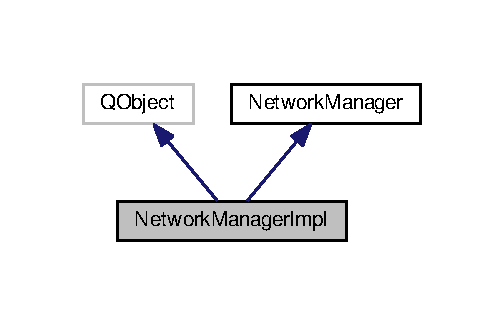
\includegraphics[width=242pt]{d8/dbf/classNetworkManagerImpl__inherit__graph}
\end{center}
\end{figure}


Collaboration diagram for Network\+Manager\+Impl\+:
\nopagebreak
\begin{figure}[H]
\begin{center}
\leavevmode
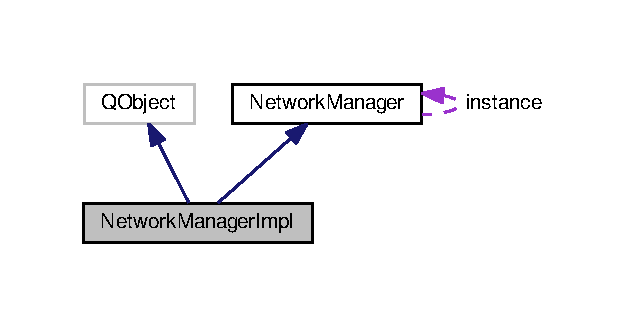
\includegraphics[width=301pt]{d2/d03/classNetworkManagerImpl__coll__graph}
\end{center}
\end{figure}
\subsection*{Public Slots}
\begin{DoxyCompactItemize}
\item 
void {\bfseries read\+Message} ()\hypertarget{classNetworkManagerImpl_a607626213287dc476d3c7bd01c076b4e}{}\label{classNetworkManagerImpl_a607626213287dc476d3c7bd01c076b4e}

\end{DoxyCompactItemize}
\subsection*{Signals}
\begin{DoxyCompactItemize}
\item 
void {\bfseries message\+Receive} (Q\+Json\+Object json\+Object) override\hypertarget{classNetworkManagerImpl_ae375fb6f5addc6325cb3a037bd9eca39}{}\label{classNetworkManagerImpl_ae375fb6f5addc6325cb3a037bd9eca39}

\end{DoxyCompactItemize}
\subsection*{Public Member Functions}
\begin{DoxyCompactItemize}
\item 
virtual void \hyperlink{classNetworkManagerImpl_a4ad2bada544bc02ea1f9921f3f6f62c2}{configure} (Q\+String \hyperlink{classNetworkManagerImpl_ac5d5c68c8000d8afef7632259e19f788}{ip}, quint16 \hyperlink{classNetworkManagerImpl_a4723f928e10d6d90987ff673b36c434d}{port}) override
\begin{DoxyCompactList}\small\item\em Método para configurar o \hyperlink{classNetworkManager}{Network\+Manager}. \end{DoxyCompactList}\item 
virtual void \hyperlink{classNetworkManagerImpl_aa468744d773aacf43763fde8e8bd95df}{login} (Q\+String username, Q\+String password) override
\begin{DoxyCompactList}\small\item\em Método para realizar um login. \end{DoxyCompactList}\item 
virtual void \hyperlink{classNetworkManagerImpl_a18fcb6129bcaa5f7f225d92ac5d6cd1c}{do\+Operation} (Q\+String username, double factor1, double factor2, int op\+Code) override
\begin{DoxyCompactList}\small\item\em Método para realizar operações matematicas. \end{DoxyCompactList}\item 
virtual void \hyperlink{classNetworkManagerImpl_aba85b7a85efee5cc28995c0df82bef5a}{report\+By\+User} (Q\+String username) override
\begin{DoxyCompactList}\small\item\em Método para recuperar o relatorio de operações do usuário. \end{DoxyCompactList}\item 
virtual void \hyperlink{classNetworkManagerImpl_a2131e26c9804d50c6e1ab6d5b7ccec94}{report\+All\+Users} (Q\+String username) override
\begin{DoxyCompactList}\small\item\em Método para recuperar o relatorio de operações de todos os usuários. \end{DoxyCompactList}\item 
virtual Q\+Object $\ast$ \hyperlink{classNetworkManagerImpl_a3340057281dadf1861d94d8aba9e976e}{get\+Q\+Object} () override
\begin{DoxyCompactList}\small\item\em Retorna um Q\+Object referente a \hyperlink{classNetworkManager}{Network\+Manager}. \end{DoxyCompactList}\end{DoxyCompactItemize}
\subsection*{Private Attributes}
\begin{DoxyCompactItemize}
\item 
Q\+String \hyperlink{classNetworkManagerImpl_ac5d5c68c8000d8afef7632259e19f788}{ip}\hypertarget{classNetworkManagerImpl_ac5d5c68c8000d8afef7632259e19f788}{}\label{classNetworkManagerImpl_ac5d5c68c8000d8afef7632259e19f788}

\begin{DoxyCompactList}\small\item\em IP do servidor. \end{DoxyCompactList}\item 
quint16 \hyperlink{classNetworkManagerImpl_a4723f928e10d6d90987ff673b36c434d}{port}\hypertarget{classNetworkManagerImpl_a4723f928e10d6d90987ff673b36c434d}{}\label{classNetworkManagerImpl_a4723f928e10d6d90987ff673b36c434d}

\begin{DoxyCompactList}\small\item\em Porta do servidor. \end{DoxyCompactList}\item 
Q\+Tcp\+Socket \hyperlink{classNetworkManagerImpl_a5b0a29db0e48c67051ec36235b1df570}{tcp\+Socket}\hypertarget{classNetworkManagerImpl_a5b0a29db0e48c67051ec36235b1df570}{}\label{classNetworkManagerImpl_a5b0a29db0e48c67051ec36235b1df570}

\begin{DoxyCompactList}\small\item\em Socket T\+CP utilizado para conexões. \end{DoxyCompactList}\end{DoxyCompactItemize}
\subsection*{Additional Inherited Members}


\subsection{Member Function Documentation}
\index{Network\+Manager\+Impl@{Network\+Manager\+Impl}!configure@{configure}}
\index{configure@{configure}!Network\+Manager\+Impl@{Network\+Manager\+Impl}}
\subsubsection[{\texorpdfstring{configure(\+Q\+String ip, quint16 port) override}{configure(QString ip, quint16 port) override}}]{\setlength{\rightskip}{0pt plus 5cm}void Network\+Manager\+Impl\+::configure (
\begin{DoxyParamCaption}
\item[{Q\+String}]{ip, }
\item[{quint16}]{port}
\end{DoxyParamCaption}
)\hspace{0.3cm}{\ttfamily [override]}, {\ttfamily [virtual]}}\hypertarget{classNetworkManagerImpl_a4ad2bada544bc02ea1f9921f3f6f62c2}{}\label{classNetworkManagerImpl_a4ad2bada544bc02ea1f9921f3f6f62c2}


Método para configurar o \hyperlink{classNetworkManager}{Network\+Manager}. 


\begin{DoxyParams}{Parameters}
{\em ip} & Ip do Servidor \\
\hline
{\em port} & Porta do Servidor \\
\hline
\end{DoxyParams}


Implements \hyperlink{classNetworkManager_ae7b073b1deb224a6cb7af0e4d3d158de}{Network\+Manager}.

\index{Network\+Manager\+Impl@{Network\+Manager\+Impl}!do\+Operation@{do\+Operation}}
\index{do\+Operation@{do\+Operation}!Network\+Manager\+Impl@{Network\+Manager\+Impl}}
\subsubsection[{\texorpdfstring{do\+Operation(\+Q\+String username, double factor1, double factor2, int op\+Code) override}{doOperation(QString username, double factor1, double factor2, int opCode) override}}]{\setlength{\rightskip}{0pt plus 5cm}void Network\+Manager\+Impl\+::do\+Operation (
\begin{DoxyParamCaption}
\item[{Q\+String}]{username, }
\item[{double}]{factor1, }
\item[{double}]{factor2, }
\item[{int}]{op\+Code}
\end{DoxyParamCaption}
)\hspace{0.3cm}{\ttfamily [override]}, {\ttfamily [virtual]}}\hypertarget{classNetworkManagerImpl_a18fcb6129bcaa5f7f225d92ac5d6cd1c}{}\label{classNetworkManagerImpl_a18fcb6129bcaa5f7f225d92ac5d6cd1c}


Método para realizar operações matematicas. 


\begin{DoxyParams}{Parameters}
{\em username} & Nome do usuário \\
\hline
{\em factor1} & Primeiro fator da operação \\
\hline
{\em factor2} & Segundo fator da operação \\
\hline
{\em op\+Code} & Código da operação \\
\hline
\end{DoxyParams}


Implements \hyperlink{classNetworkManager_a7477e7bdee53e76ead1b711d2976e1e1}{Network\+Manager}.

\index{Network\+Manager\+Impl@{Network\+Manager\+Impl}!get\+Q\+Object@{get\+Q\+Object}}
\index{get\+Q\+Object@{get\+Q\+Object}!Network\+Manager\+Impl@{Network\+Manager\+Impl}}
\subsubsection[{\texorpdfstring{get\+Q\+Object() override}{getQObject() override}}]{\setlength{\rightskip}{0pt plus 5cm}Q\+Object $\ast$ Network\+Manager\+Impl\+::get\+Q\+Object (
\begin{DoxyParamCaption}
{}
\end{DoxyParamCaption}
)\hspace{0.3cm}{\ttfamily [override]}, {\ttfamily [virtual]}}\hypertarget{classNetworkManagerImpl_a3340057281dadf1861d94d8aba9e976e}{}\label{classNetworkManagerImpl_a3340057281dadf1861d94d8aba9e976e}


Retorna um Q\+Object referente a \hyperlink{classNetworkManager}{Network\+Manager}. 

\begin{DoxyReturn}{Returns}
Q\+Object correspondente 
\end{DoxyReturn}


Implements \hyperlink{classNetworkManager_a437755d5e84ea8522515283ba11f4b77}{Network\+Manager}.

\index{Network\+Manager\+Impl@{Network\+Manager\+Impl}!login@{login}}
\index{login@{login}!Network\+Manager\+Impl@{Network\+Manager\+Impl}}
\subsubsection[{\texorpdfstring{login(\+Q\+String username, Q\+String password) override}{login(QString username, QString password) override}}]{\setlength{\rightskip}{0pt plus 5cm}void Network\+Manager\+Impl\+::login (
\begin{DoxyParamCaption}
\item[{Q\+String}]{username, }
\item[{Q\+String}]{password}
\end{DoxyParamCaption}
)\hspace{0.3cm}{\ttfamily [override]}, {\ttfamily [virtual]}}\hypertarget{classNetworkManagerImpl_aa468744d773aacf43763fde8e8bd95df}{}\label{classNetworkManagerImpl_aa468744d773aacf43763fde8e8bd95df}


Método para realizar um login. 


\begin{DoxyParams}{Parameters}
{\em username} & Nome do usuário \\
\hline
{\em password} & Senha do usuário \\
\hline
\end{DoxyParams}


Implements \hyperlink{classNetworkManager_ad39555f78185618bb5e6e906a9ef0c40}{Network\+Manager}.

\index{Network\+Manager\+Impl@{Network\+Manager\+Impl}!report\+All\+Users@{report\+All\+Users}}
\index{report\+All\+Users@{report\+All\+Users}!Network\+Manager\+Impl@{Network\+Manager\+Impl}}
\subsubsection[{\texorpdfstring{report\+All\+Users(\+Q\+String username) override}{reportAllUsers(QString username) override}}]{\setlength{\rightskip}{0pt plus 5cm}void Network\+Manager\+Impl\+::report\+All\+Users (
\begin{DoxyParamCaption}
\item[{Q\+String}]{username}
\end{DoxyParamCaption}
)\hspace{0.3cm}{\ttfamily [override]}, {\ttfamily [virtual]}}\hypertarget{classNetworkManagerImpl_a2131e26c9804d50c6e1ab6d5b7ccec94}{}\label{classNetworkManagerImpl_a2131e26c9804d50c6e1ab6d5b7ccec94}


Método para recuperar o relatorio de operações de todos os usuários. 


\begin{DoxyParams}{Parameters}
{\em username} & Nome do usuário solicitando \\
\hline
\end{DoxyParams}
\begin{DoxySeeAlso}{See also}
\hyperlink{classNetworkManager_a1d37ebe528cb047d40bbacd950e0ef83}{Network\+Manager\+::report\+By\+User()} 
\end{DoxySeeAlso}


Implements \hyperlink{classNetworkManager_a8c788f00be9ce6736cf3a1deac0b0906}{Network\+Manager}.

\index{Network\+Manager\+Impl@{Network\+Manager\+Impl}!report\+By\+User@{report\+By\+User}}
\index{report\+By\+User@{report\+By\+User}!Network\+Manager\+Impl@{Network\+Manager\+Impl}}
\subsubsection[{\texorpdfstring{report\+By\+User(\+Q\+String username) override}{reportByUser(QString username) override}}]{\setlength{\rightskip}{0pt plus 5cm}void Network\+Manager\+Impl\+::report\+By\+User (
\begin{DoxyParamCaption}
\item[{Q\+String}]{username}
\end{DoxyParamCaption}
)\hspace{0.3cm}{\ttfamily [override]}, {\ttfamily [virtual]}}\hypertarget{classNetworkManagerImpl_aba85b7a85efee5cc28995c0df82bef5a}{}\label{classNetworkManagerImpl_aba85b7a85efee5cc28995c0df82bef5a}


Método para recuperar o relatorio de operações do usuário. 


\begin{DoxyParams}{Parameters}
{\em username} & Nome do usuário a ser gerado o relatorio \\
\hline
\end{DoxyParams}
\begin{DoxySeeAlso}{See also}
\hyperlink{classNetworkManager_a8c788f00be9ce6736cf3a1deac0b0906}{Network\+Manager\+::report\+All\+Users()} 
\end{DoxySeeAlso}


Implements \hyperlink{classNetworkManager_a1d37ebe528cb047d40bbacd950e0ef83}{Network\+Manager}.



The documentation for this class was generated from the following files\+:\begin{DoxyCompactItemize}
\item 
Calc\+Client/src/control/\hyperlink{networkmanagerimpl_8h}{networkmanagerimpl.\+h}\item 
Calc\+Client/src/control/\hyperlink{networkmanagerimpl_8cpp}{networkmanagerimpl.\+cpp}\end{DoxyCompactItemize}

\hypertarget{classRole}{}\section{Role Class Reference}
\label{classRole}\index{Role@{Role}}


Superclasse correspondente aos papeis que podem ser assumidos no sistema.  




{\ttfamily \#include $<$role.\+h$>$}



Inheritance diagram for Role\+:
\nopagebreak
\begin{figure}[H]
\begin{center}
\leavevmode
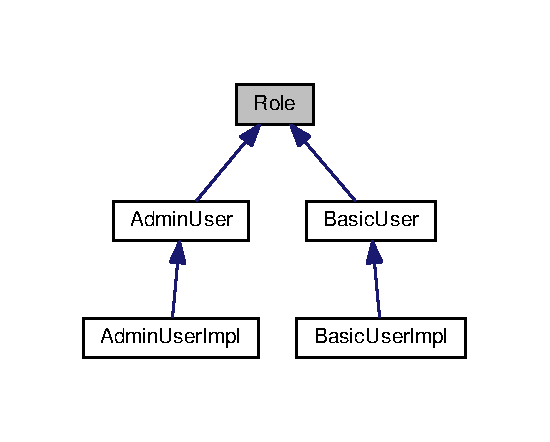
\includegraphics[width=264pt]{d3/d43/classRole__inherit__graph}
\end{center}
\end{figure}
\subsection*{Public Member Functions}
\begin{DoxyCompactItemize}
\item 
virtual Q\+String \hyperlink{classRole_a295daeaed997d10f9bd3d03e972318c1}{get\+Role\+Name} ()=0
\begin{DoxyCompactList}\small\item\em Método para acessar o nome papel. \end{DoxyCompactList}\item 
virtual \hyperlink{classUser}{User} $\ast$ \hyperlink{classRole_abad7de00bc38b11eaae8a79069773221}{get\+User} ()=0
\begin{DoxyCompactList}\small\item\em Método para acessar o usuário correspondente ao papel. \end{DoxyCompactList}\item 
virtual void \hyperlink{classRole_ab5581d91192fa578070e80b0247dde5a}{set\+User} (\hyperlink{classUser}{User} $\ast$user)=0
\begin{DoxyCompactList}\small\item\em Método para associar um usuário a um papel. \end{DoxyCompactList}\end{DoxyCompactItemize}


\subsection{Detailed Description}
Superclasse correspondente aos papeis que podem ser assumidos no sistema. 

\subsection{Member Function Documentation}
\index{Role@{Role}!get\+Role\+Name@{get\+Role\+Name}}
\index{get\+Role\+Name@{get\+Role\+Name}!Role@{Role}}
\subsubsection[{\texorpdfstring{get\+Role\+Name()=0}{getRoleName()=0}}]{\setlength{\rightskip}{0pt plus 5cm}virtual Q\+String Role\+::get\+Role\+Name (
\begin{DoxyParamCaption}
{}
\end{DoxyParamCaption}
)\hspace{0.3cm}{\ttfamily [pure virtual]}}\hypertarget{classRole_a295daeaed997d10f9bd3d03e972318c1}{}\label{classRole_a295daeaed997d10f9bd3d03e972318c1}


Método para acessar o nome papel. 

\begin{DoxyReturn}{Returns}
Nome do papel 
\end{DoxyReturn}


Implemented in \hyperlink{classAdminUserImpl_a8fc6881cf92e783065001be43209a5a6}{Admin\+User\+Impl}, and \hyperlink{classBasicUserImpl_aaf68b785533f15a61fa30cdef3c82145}{Basic\+User\+Impl}.

\index{Role@{Role}!get\+User@{get\+User}}
\index{get\+User@{get\+User}!Role@{Role}}
\subsubsection[{\texorpdfstring{get\+User()=0}{getUser()=0}}]{\setlength{\rightskip}{0pt plus 5cm}virtual {\bf User}$\ast$ Role\+::get\+User (
\begin{DoxyParamCaption}
{}
\end{DoxyParamCaption}
)\hspace{0.3cm}{\ttfamily [pure virtual]}}\hypertarget{classRole_abad7de00bc38b11eaae8a79069773221}{}\label{classRole_abad7de00bc38b11eaae8a79069773221}


Método para acessar o usuário correspondente ao papel. 

\begin{DoxyReturn}{Returns}
Usuário associado ao papel 
\end{DoxyReturn}


Implemented in \hyperlink{classAdminUserImpl_aa548616e5bf99062155ee397bf9be6ad}{Admin\+User\+Impl}, and \hyperlink{classBasicUserImpl_ace1ba87379b0b3817a089d6933dc0dd7}{Basic\+User\+Impl}.

\index{Role@{Role}!set\+User@{set\+User}}
\index{set\+User@{set\+User}!Role@{Role}}
\subsubsection[{\texorpdfstring{set\+User(\+User $\ast$user)=0}{setUser(User *user)=0}}]{\setlength{\rightskip}{0pt plus 5cm}virtual void Role\+::set\+User (
\begin{DoxyParamCaption}
\item[{{\bf User} $\ast$}]{user}
\end{DoxyParamCaption}
)\hspace{0.3cm}{\ttfamily [pure virtual]}}\hypertarget{classRole_ab5581d91192fa578070e80b0247dde5a}{}\label{classRole_ab5581d91192fa578070e80b0247dde5a}


Método para associar um usuário a um papel. 


\begin{DoxyParams}{Parameters}
{\em user} & Usuário a ser associado \\
\hline
\end{DoxyParams}


Implemented in \hyperlink{classAdminUserImpl_a5a392bdfba62518e31e40819fe3c32b7}{Admin\+User\+Impl}, and \hyperlink{classBasicUserImpl_af94875b3b06f1f1effc3a58fce087e5d}{Basic\+User\+Impl}.



The documentation for this class was generated from the following file\+:\begin{DoxyCompactItemize}
\item 
Calc\+Client/src/data/\hyperlink{role_8h}{role.\+h}\end{DoxyCompactItemize}

\hypertarget{classServer}{}\section{Server Class Reference}
\label{classServer}\index{Server@{Server}}


Clase para gerenciamento de servidor T\+CP.  




{\ttfamily \#include $<$server.\+h$>$}



Inheritance diagram for Server\+:\nopagebreak
\begin{figure}[H]
\begin{center}
\leavevmode
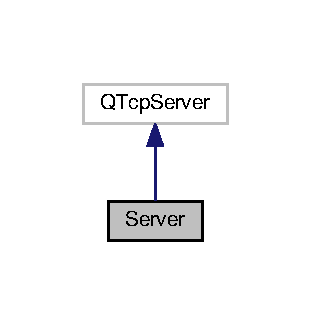
\includegraphics[width=149pt]{d3/dd7/classServer__inherit__graph}
\end{center}
\end{figure}


Collaboration diagram for Server\+:\nopagebreak
\begin{figure}[H]
\begin{center}
\leavevmode
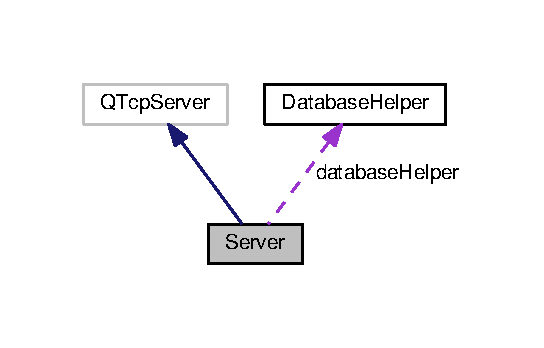
\includegraphics[width=149pt]{de/ddc/classServer__coll__graph}
\end{center}
\end{figure}
\subsection*{Protected Member Functions}
\begin{DoxyCompactItemize}
\item 
virtual void \hyperlink{classServer_a2397527620515d7e18fc599b22fb64ae}{incoming\+Connection} (qintptr socket\+Descriptor)=0
\begin{DoxyCompactList}\small\item\em Método para delegar o tratamento de uma conexão a uma thread trabalhadora auxiliar. \end{DoxyCompactList}\end{DoxyCompactItemize}


\subsection{Detailed Description}
Clase para gerenciamento de servidor T\+CP. 

\subsection{Member Function Documentation}
\index{Server@{Server}!incoming\+Connection@{incoming\+Connection}}
\index{incoming\+Connection@{incoming\+Connection}!Server@{Server}}
\subsubsection[{\texorpdfstring{incoming\+Connection(qintptr socket\+Descriptor)=0}{incomingConnection(qintptr socketDescriptor)=0}}]{\setlength{\rightskip}{0pt plus 5cm}virtual void Server\+::incoming\+Connection (
\begin{DoxyParamCaption}
\item[{qintptr}]{socket\+Descriptor}
\end{DoxyParamCaption}
)\hspace{0.3cm}{\ttfamily [protected]}, {\ttfamily [pure virtual]}}\hypertarget{classServer_a2397527620515d7e18fc599b22fb64ae}{}\label{classServer_a2397527620515d7e18fc599b22fb64ae}


Método para delegar o tratamento de uma conexão a uma thread trabalhadora auxiliar. 

Ao receber uma conexão o servidor delega o tratamento dela a um thread auxiliar e volta a escutar as transmissões.


\begin{DoxyParams}{Parameters}
{\em socket\+Descriptor} & Informações de configuração do socket.\\
\hline
\end{DoxyParams}
\begin{DoxySeeAlso}{See also}
\hyperlink{classWorkerThread}{Worker\+Thread}. 
\end{DoxySeeAlso}


Implemented in \hyperlink{classServerImpl_a54dda38486e9964432b501f7da00ed97}{Server\+Impl}.



The documentation for this class was generated from the following file\+:\begin{DoxyCompactItemize}
\item 
Calc\+Server/\hyperlink{server_8h}{server.\+h}\end{DoxyCompactItemize}

\hypertarget{classServerDialog}{}\section{Server\+Dialog Class Reference}
\label{classServerDialog}\index{Server\+Dialog@{Server\+Dialog}}


Classe para exibição dos dados do servidor.  




{\ttfamily \#include $<$serverdialog.\+h$>$}



Inheritance diagram for Server\+Dialog\+:\nopagebreak
\begin{figure}[H]
\begin{center}
\leavevmode
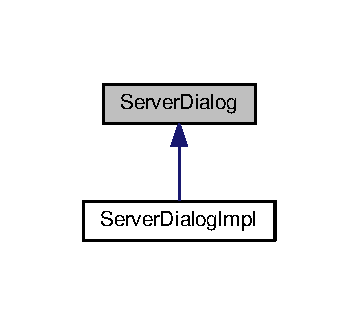
\includegraphics[width=172pt]{d2/d7c/classServerDialog__inherit__graph}
\end{center}
\end{figure}


Collaboration diagram for Server\+Dialog\+:\nopagebreak
\begin{figure}[H]
\begin{center}
\leavevmode
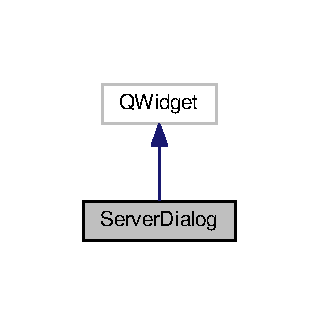
\includegraphics[width=153pt]{da/d23/classServerDialog__coll__graph}
\end{center}
\end{figure}


\subsection{Detailed Description}
Classe para exibição dos dados do servidor. 

The documentation for this class was generated from the following file\+:\begin{DoxyCompactItemize}
\item 
Calc\+Server/\hyperlink{serverdialog_8h}{serverdialog.\+h}\end{DoxyCompactItemize}

\hypertarget{classServerDialogImpl}{}\section{Server\+Dialog\+Impl Class Reference}
\label{classServerDialogImpl}\index{Server\+Dialog\+Impl@{Server\+Dialog\+Impl}}


Implementação da interface \hyperlink{classServerDialog}{Server\+Dialog}.  




{\ttfamily \#include $<$serverdialogimpl.\+h$>$}



Inheritance diagram for Server\+Dialog\+Impl\+:
\nopagebreak
\begin{figure}[H]
\begin{center}
\leavevmode
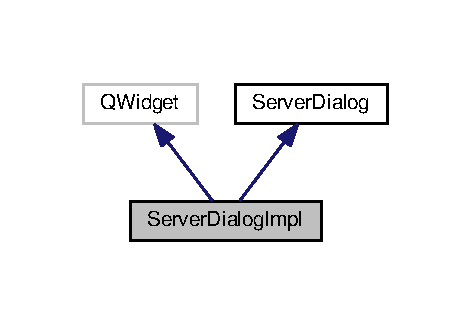
\includegraphics[width=226pt]{d1/da5/classServerDialogImpl__inherit__graph}
\end{center}
\end{figure}


Collaboration diagram for Server\+Dialog\+Impl\+:
\nopagebreak
\begin{figure}[H]
\begin{center}
\leavevmode
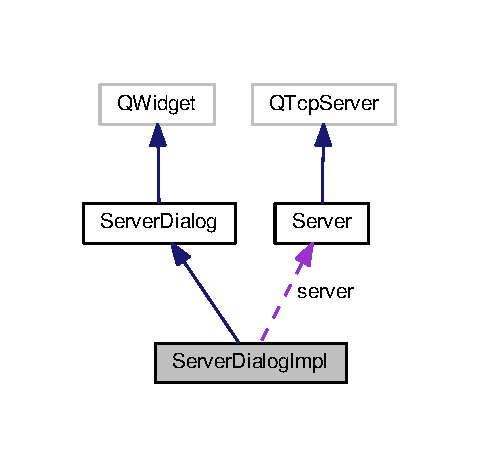
\includegraphics[width=289pt]{d3/d6b/classServerDialogImpl__coll__graph}
\end{center}
\end{figure}
\subsection*{Public Member Functions}
\begin{DoxyCompactItemize}
\item 
\hyperlink{classServerDialogImpl_a5a5cf39e32c0559a8fcdeb372fb055b3}{Server\+Dialog\+Impl} (Q\+Widget $\ast$parent=nullptr)
\begin{DoxyCompactList}\small\item\em Construtor padrão da classe \hyperlink{classServerDialogImpl}{Server\+Dialog\+Impl}. \end{DoxyCompactList}\item 
virtual \hyperlink{classServerDialogImpl_a0e73fbf7d75d033ec4ec12dc93931952}{$\sim$\+Server\+Dialog\+Impl} ()\hypertarget{classServerDialogImpl_a0e73fbf7d75d033ec4ec12dc93931952}{}\label{classServerDialogImpl_a0e73fbf7d75d033ec4ec12dc93931952}

\begin{DoxyCompactList}\small\item\em Destrutor da classe \hyperlink{classServerDialogImpl}{Server\+Dialog\+Impl}. \end{DoxyCompactList}\item 
virtual void \hyperlink{classServerDialogImpl_a6d84adfcfb187c124cc9a0a73a17c44d}{show} ()
\begin{DoxyCompactList}\small\item\em Método que exibe um janela de dialogo com as informações do server. \end{DoxyCompactList}\end{DoxyCompactItemize}
\subsection*{Private Member Functions}
\begin{DoxyCompactItemize}
\item 
\hyperlink{classServerDialogImpl_adab2dead3a4b7e4890cd53c7309cdc4c}{Server\+Dialog\+Impl} (const \hyperlink{classServerDialogImpl}{Server\+Dialog\+Impl} \&rhs)
\begin{DoxyCompactList}\small\item\em Construtor de Cópia. \end{DoxyCompactList}\item 
\hyperlink{classServerDialogImpl}{Server\+Dialog\+Impl} \& \hyperlink{classServerDialogImpl_a82cff5544b91edcd872b1a11f78c68d4}{operator=} (const \hyperlink{classServerDialogImpl}{Server\+Dialog\+Impl} \&rhs)
\begin{DoxyCompactList}\small\item\em Sobrecarga do operador =. \end{DoxyCompactList}\end{DoxyCompactItemize}
\subsection*{Private Attributes}
\begin{DoxyCompactItemize}
\item 
Q\+Label $\ast$ \hyperlink{classServerDialogImpl_a939de93eb188fe551041eb94531072af}{status\+Label}\hypertarget{classServerDialogImpl_a939de93eb188fe551041eb94531072af}{}\label{classServerDialogImpl_a939de93eb188fe551041eb94531072af}

\begin{DoxyCompactList}\small\item\em Q\+Label para exibição dos dados do servidor. \end{DoxyCompactList}\item 
Q\+Push\+Button $\ast$ \hyperlink{classServerDialogImpl_a620d45dc0aca6115b54502cf4939fa60}{quit\+Button}\hypertarget{classServerDialogImpl_a620d45dc0aca6115b54502cf4939fa60}{}\label{classServerDialogImpl_a620d45dc0aca6115b54502cf4939fa60}

\begin{DoxyCompactList}\small\item\em Botão de sair da aplicação. \end{DoxyCompactList}\item 
\hyperlink{classServer}{Server} $\ast$ \hyperlink{classServerDialogImpl_ad69d13de3b1f89c826bb5a5c82ee91fb}{server}\hypertarget{classServerDialogImpl_ad69d13de3b1f89c826bb5a5c82ee91fb}{}\label{classServerDialogImpl_ad69d13de3b1f89c826bb5a5c82ee91fb}

\begin{DoxyCompactList}\small\item\em Instância de \hyperlink{classServer}{Server}. \end{DoxyCompactList}\end{DoxyCompactItemize}
\subsection*{Friends}
\begin{DoxyCompactItemize}
\item 
class \hyperlink{classServerDialogImpl_a9fe923be634f4d12f5a825141fafb85f}{Dialog\+Test}\hypertarget{classServerDialogImpl_a9fe923be634f4d12f5a825141fafb85f}{}\label{classServerDialogImpl_a9fe923be634f4d12f5a825141fafb85f}

\begin{DoxyCompactList}\small\item\em Classe de Testes para \hyperlink{classServerDialog}{Server\+Dialog}. \end{DoxyCompactList}\item 
class \hyperlink{classServerDialogImpl_a9c408e8dbdb17dca5ff54b16daeed3f6}{Sockets\+Test}\hypertarget{classServerDialogImpl_a9c408e8dbdb17dca5ff54b16daeed3f6}{}\label{classServerDialogImpl_a9c408e8dbdb17dca5ff54b16daeed3f6}

\begin{DoxyCompactList}\small\item\em Classe de Testes para Sockets. \end{DoxyCompactList}\end{DoxyCompactItemize}


\subsection{Detailed Description}
Implementação da interface \hyperlink{classServerDialog}{Server\+Dialog}. 

Esta classe cria uma instância de \hyperlink{classServer}{Server} e exibe suas informações. 

\subsection{Constructor \& Destructor Documentation}
\index{Server\+Dialog\+Impl@{Server\+Dialog\+Impl}!Server\+Dialog\+Impl@{Server\+Dialog\+Impl}}
\index{Server\+Dialog\+Impl@{Server\+Dialog\+Impl}!Server\+Dialog\+Impl@{Server\+Dialog\+Impl}}
\subsubsection[{\texorpdfstring{Server\+Dialog\+Impl(\+Q\+Widget $\ast$parent=nullptr)}{ServerDialogImpl(QWidget *parent=nullptr)}}]{\setlength{\rightskip}{0pt plus 5cm}Server\+Dialog\+Impl\+::\+Server\+Dialog\+Impl (
\begin{DoxyParamCaption}
\item[{Q\+Widget $\ast$}]{parent = {\ttfamily nullptr}}
\end{DoxyParamCaption}
)}\hypertarget{classServerDialogImpl_a5a5cf39e32c0559a8fcdeb372fb055b3}{}\label{classServerDialogImpl_a5a5cf39e32c0559a8fcdeb372fb055b3}


Construtor padrão da classe \hyperlink{classServerDialogImpl}{Server\+Dialog\+Impl}. 

Instância e configura a interface. Além disso configura a instância de \hyperlink{classServer}{Server} antes de deixa-\/la tratando as requisições.


\begin{DoxyParams}{Parameters}
{\em parent} & Referência ao componente pai. \\
\hline
\end{DoxyParams}
\index{Server\+Dialog\+Impl@{Server\+Dialog\+Impl}!Server\+Dialog\+Impl@{Server\+Dialog\+Impl}}
\index{Server\+Dialog\+Impl@{Server\+Dialog\+Impl}!Server\+Dialog\+Impl@{Server\+Dialog\+Impl}}
\subsubsection[{\texorpdfstring{Server\+Dialog\+Impl(const Server\+Dialog\+Impl \&rhs)}{ServerDialogImpl(const ServerDialogImpl &rhs)}}]{\setlength{\rightskip}{0pt plus 5cm}Server\+Dialog\+Impl\+::\+Server\+Dialog\+Impl (
\begin{DoxyParamCaption}
\item[{const {\bf Server\+Dialog\+Impl} \&}]{rhs}
\end{DoxyParamCaption}
)\hspace{0.3cm}{\ttfamily [private]}}\hypertarget{classServerDialogImpl_adab2dead3a4b7e4890cd53c7309cdc4c}{}\label{classServerDialogImpl_adab2dead3a4b7e4890cd53c7309cdc4c}


Construtor de Cópia. 


\begin{DoxyParams}{Parameters}
{\em rhs} & Objeto a ser copiado. \\
\hline
\end{DoxyParams}


\subsection{Member Function Documentation}
\index{Server\+Dialog\+Impl@{Server\+Dialog\+Impl}!operator=@{operator=}}
\index{operator=@{operator=}!Server\+Dialog\+Impl@{Server\+Dialog\+Impl}}
\subsubsection[{\texorpdfstring{operator=(const Server\+Dialog\+Impl \&rhs)}{operator=(const ServerDialogImpl &rhs)}}]{\setlength{\rightskip}{0pt plus 5cm}{\bf Server\+Dialog\+Impl} \& Server\+Dialog\+Impl\+::operator= (
\begin{DoxyParamCaption}
\item[{const {\bf Server\+Dialog\+Impl} \&}]{rhs}
\end{DoxyParamCaption}
)\hspace{0.3cm}{\ttfamily [private]}}\hypertarget{classServerDialogImpl_a82cff5544b91edcd872b1a11f78c68d4}{}\label{classServerDialogImpl_a82cff5544b91edcd872b1a11f78c68d4}


Sobrecarga do operador =. 


\begin{DoxyParams}{Parameters}
{\em rhs} & Objeto a ser copiado. \\
\hline
\end{DoxyParams}
\begin{DoxyReturn}{Returns}
Novo objeto copiado. 
\end{DoxyReturn}
\index{Server\+Dialog\+Impl@{Server\+Dialog\+Impl}!show@{show}}
\index{show@{show}!Server\+Dialog\+Impl@{Server\+Dialog\+Impl}}
\subsubsection[{\texorpdfstring{show()}{show()}}]{\setlength{\rightskip}{0pt plus 5cm}void Server\+Dialog\+Impl\+::show (
\begin{DoxyParamCaption}
{}
\end{DoxyParamCaption}
)\hspace{0.3cm}{\ttfamily [virtual]}}\hypertarget{classServerDialogImpl_a6d84adfcfb187c124cc9a0a73a17c44d}{}\label{classServerDialogImpl_a6d84adfcfb187c124cc9a0a73a17c44d}


Método que exibe um janela de dialogo com as informações do server. 

\begin{DoxySeeAlso}{See also}
\hyperlink{classServer}{Server}. 
\end{DoxySeeAlso}


Implements \hyperlink{classServerDialog_a79906f2c91c29b2504c2cb370d302b00}{Server\+Dialog}.



The documentation for this class was generated from the following files\+:\begin{DoxyCompactItemize}
\item 
Calc\+Server/src/gui/\hyperlink{serverdialogimpl_8h}{serverdialogimpl.\+h}\item 
Calc\+Server/src/gui/\hyperlink{serverdialogimpl_8cpp}{serverdialogimpl.\+cpp}\end{DoxyCompactItemize}

\hypertarget{classServerImpl}{}\section{Server\+Impl Class Reference}
\label{classServerImpl}\index{Server\+Impl@{Server\+Impl}}


Implementação da interface \hyperlink{classServer}{Server}.  




{\ttfamily \#include $<$serverimpl.\+h$>$}



Inheritance diagram for Server\+Impl\+:\nopagebreak
\begin{figure}[H]
\begin{center}
\leavevmode
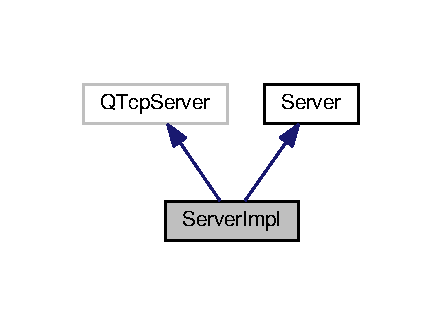
\includegraphics[width=212pt]{d3/da0/classServerImpl__inherit__graph}
\end{center}
\end{figure}


Collaboration diagram for Server\+Impl\+:\nopagebreak
\begin{figure}[H]
\begin{center}
\leavevmode
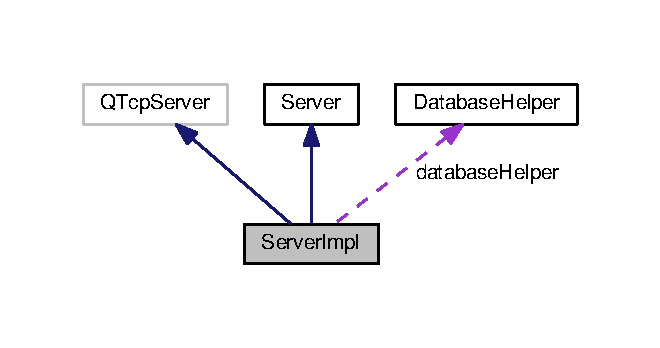
\includegraphics[width=317pt]{de/d15/classServerImpl__coll__graph}
\end{center}
\end{figure}
\subsection*{Public Member Functions}
\begin{DoxyCompactItemize}
\item 
\hyperlink{classServerImpl_a0c81e2a5af6cea9a1ff0445008c22e84}{Server\+Impl} (Q\+Object $\ast$parent=nullptr)
\begin{DoxyCompactList}\small\item\em Construtor padrão da classe \hyperlink{classServerImpl}{Server\+Impl}. \end{DoxyCompactList}\item 
virtual \hyperlink{classServerImpl_aef0bf73c21130de67a3f262dff915cd2}{$\sim$\+Server\+Impl} () override
\begin{DoxyCompactList}\small\item\em Destrutor da classe \hyperlink{classServerImpl}{Server\+Impl}. \end{DoxyCompactList}\item 
virtual bool \hyperlink{classServerImpl_a3a186b4e86c634750f8fb95f962d5ec9}{listen} () override
\begin{DoxyCompactList}\small\item\em Método para escutar conexões ao server. \end{DoxyCompactList}\item 
virtual Q\+String \hyperlink{classServerImpl_aaadf6ebb053052ee61303848374e8d20}{error\+String} () const override
\begin{DoxyCompactList}\small\item\em Método que retorna a mensagem referente ao último erro do server. \end{DoxyCompactList}\item 
virtual quint16 \hyperlink{classServerImpl_a769680151e32d74aeae35dfbb1dcbde0}{server\+Port} () const override
\begin{DoxyCompactList}\small\item\em Método que informa a porta a qual o servidor está escutando. \end{DoxyCompactList}\end{DoxyCompactItemize}
\subsection*{Protected Member Functions}
\begin{DoxyCompactItemize}
\item 
void \hyperlink{classServerImpl_a54dda38486e9964432b501f7da00ed97}{incoming\+Connection} (qintptr socket\+Descriptor) override
\begin{DoxyCompactList}\small\item\em Método para delegar o tratamento de uma conexão a uma thread trabalhadora auxiliar. \end{DoxyCompactList}\item 
\hyperlink{classServerImpl_ad288c40b899759a72121cbcd60817cf9}{Server\+Impl} (const \hyperlink{classServerImpl}{Server\+Impl} \&rhs)
\begin{DoxyCompactList}\small\item\em Construtor de Cópia. \end{DoxyCompactList}\item 
\hyperlink{classServerImpl}{Server\+Impl} \& \hyperlink{classServerImpl_aa3cc217c7588777ec4deb99132f847ef}{operator=} (const \hyperlink{classServerImpl}{Server\+Impl} \&rhs)
\begin{DoxyCompactList}\small\item\em Sobrecarga do operador =. \end{DoxyCompactList}\end{DoxyCompactItemize}
\subsection*{Protected Attributes}
\begin{DoxyCompactItemize}
\item 
\hyperlink{classDatabaseHelper}{Database\+Helper} $\ast$ \hyperlink{classServerImpl_af78b294c790b327b0023f295c5d7508c}{database\+Helper}\hypertarget{classServerImpl_af78b294c790b327b0023f295c5d7508c}{}\label{classServerImpl_af78b294c790b327b0023f295c5d7508c}

\begin{DoxyCompactList}\small\item\em Referência ao helper de acesso ao banco de dados. \end{DoxyCompactList}\end{DoxyCompactItemize}


\subsection{Detailed Description}
Implementação da interface \hyperlink{classServer}{Server}. 

\subsection{Constructor \& Destructor Documentation}
\index{Server\+Impl@{Server\+Impl}!Server\+Impl@{Server\+Impl}}
\index{Server\+Impl@{Server\+Impl}!Server\+Impl@{Server\+Impl}}
\subsubsection[{\texorpdfstring{Server\+Impl(\+Q\+Object $\ast$parent=nullptr)}{ServerImpl(QObject *parent=nullptr)}}]{\setlength{\rightskip}{0pt plus 5cm}Server\+Impl\+::\+Server\+Impl (
\begin{DoxyParamCaption}
\item[{Q\+Object $\ast$}]{parent = {\ttfamily nullptr}}
\end{DoxyParamCaption}
)}\hypertarget{classServerImpl_a0c81e2a5af6cea9a1ff0445008c22e84}{}\label{classServerImpl_a0c81e2a5af6cea9a1ff0445008c22e84}


Construtor padrão da classe \hyperlink{classServerImpl}{Server\+Impl}. 

Demanda a configuração do \hyperlink{classServer}{Server} para a classe pai e instância um helper de acesso ao banco de dados.


\begin{DoxyParams}{Parameters}
{\em parent} & Referência ao componente pai. \\
\hline
\end{DoxyParams}
\index{Server\+Impl@{Server\+Impl}!````~Server\+Impl@{$\sim$\+Server\+Impl}}
\index{````~Server\+Impl@{$\sim$\+Server\+Impl}!Server\+Impl@{Server\+Impl}}
\subsubsection[{\texorpdfstring{$\sim$\+Server\+Impl() override}{~ServerImpl() override}}]{\setlength{\rightskip}{0pt plus 5cm}Server\+Impl\+::$\sim$\+Server\+Impl (
\begin{DoxyParamCaption}
{}
\end{DoxyParamCaption}
)\hspace{0.3cm}{\ttfamily [override]}, {\ttfamily [virtual]}}\hypertarget{classServerImpl_aef0bf73c21130de67a3f262dff915cd2}{}\label{classServerImpl_aef0bf73c21130de67a3f262dff915cd2}


Destrutor da classe \hyperlink{classServerImpl}{Server\+Impl}. 

Apaga a referência ao helper de acesso ao banco de dados. \index{Server\+Impl@{Server\+Impl}!Server\+Impl@{Server\+Impl}}
\index{Server\+Impl@{Server\+Impl}!Server\+Impl@{Server\+Impl}}
\subsubsection[{\texorpdfstring{Server\+Impl(const Server\+Impl \&rhs)}{ServerImpl(const ServerImpl &rhs)}}]{\setlength{\rightskip}{0pt plus 5cm}Server\+Impl\+::\+Server\+Impl (
\begin{DoxyParamCaption}
\item[{const {\bf Server\+Impl} \&}]{rhs}
\end{DoxyParamCaption}
)\hspace{0.3cm}{\ttfamily [protected]}}\hypertarget{classServerImpl_ad288c40b899759a72121cbcd60817cf9}{}\label{classServerImpl_ad288c40b899759a72121cbcd60817cf9}


Construtor de Cópia. 


\begin{DoxyParams}{Parameters}
{\em rhs} & Objeto a ser copiado. \\
\hline
\end{DoxyParams}


\subsection{Member Function Documentation}
\index{Server\+Impl@{Server\+Impl}!error\+String@{error\+String}}
\index{error\+String@{error\+String}!Server\+Impl@{Server\+Impl}}
\subsubsection[{\texorpdfstring{error\+String() const override}{errorString() const override}}]{\setlength{\rightskip}{0pt plus 5cm}Q\+String Server\+Impl\+::error\+String (
\begin{DoxyParamCaption}
{}
\end{DoxyParamCaption}
) const\hspace{0.3cm}{\ttfamily [override]}, {\ttfamily [virtual]}}\hypertarget{classServerImpl_aaadf6ebb053052ee61303848374e8d20}{}\label{classServerImpl_aaadf6ebb053052ee61303848374e8d20}


Método que retorna a mensagem referente ao último erro do server. 

\begin{DoxyReturn}{Returns}
Mensagem de erro. 
\end{DoxyReturn}


Implements \hyperlink{classServer_a66eb77ac2362bdae05081591389c3cf5}{Server}.

\index{Server\+Impl@{Server\+Impl}!incoming\+Connection@{incoming\+Connection}}
\index{incoming\+Connection@{incoming\+Connection}!Server\+Impl@{Server\+Impl}}
\subsubsection[{\texorpdfstring{incoming\+Connection(qintptr socket\+Descriptor) override}{incomingConnection(qintptr socketDescriptor) override}}]{\setlength{\rightskip}{0pt plus 5cm}void Server\+Impl\+::incoming\+Connection (
\begin{DoxyParamCaption}
\item[{qintptr}]{socket\+Descriptor}
\end{DoxyParamCaption}
)\hspace{0.3cm}{\ttfamily [override]}, {\ttfamily [protected]}, {\ttfamily [virtual]}}\hypertarget{classServerImpl_a54dda38486e9964432b501f7da00ed97}{}\label{classServerImpl_a54dda38486e9964432b501f7da00ed97}


Método para delegar o tratamento de uma conexão a uma thread trabalhadora auxiliar. 

Ao receber uma conexão o servidor delega o tratamento dela a um thread auxiliar e volta a escutar as transmissões.


\begin{DoxyParams}{Parameters}
{\em socket\+Descriptor} & Informações de configuração do socket.\\
\hline
\end{DoxyParams}
\begin{DoxySeeAlso}{See also}
\hyperlink{classWorkerThread}{Worker\+Thread}. 
\end{DoxySeeAlso}


Implements \hyperlink{classServer_a2397527620515d7e18fc599b22fb64ae}{Server}.

\index{Server\+Impl@{Server\+Impl}!listen@{listen}}
\index{listen@{listen}!Server\+Impl@{Server\+Impl}}
\subsubsection[{\texorpdfstring{listen() override}{listen() override}}]{\setlength{\rightskip}{0pt plus 5cm}bool Server\+Impl\+::listen (
\begin{DoxyParamCaption}
{}
\end{DoxyParamCaption}
)\hspace{0.3cm}{\ttfamily [override]}, {\ttfamily [virtual]}}\hypertarget{classServerImpl_a3a186b4e86c634750f8fb95f962d5ec9}{}\label{classServerImpl_a3a186b4e86c634750f8fb95f962d5ec9}


Método para escutar conexões ao server. 

Esse método instancia um listener em um ip e porta do computador. Caso consiga retorna verdadeiro, caso contrário, retorna falso.

\begin{DoxySeeAlso}{See also}
\hyperlink{classServerDialog}{Server\+Dialog} 
\end{DoxySeeAlso}


Implements \hyperlink{classServer_a2393cde56bb44076cbfba00c89412acf}{Server}.

\index{Server\+Impl@{Server\+Impl}!operator=@{operator=}}
\index{operator=@{operator=}!Server\+Impl@{Server\+Impl}}
\subsubsection[{\texorpdfstring{operator=(const Server\+Impl \&rhs)}{operator=(const ServerImpl &rhs)}}]{\setlength{\rightskip}{0pt plus 5cm}{\bf Server\+Impl} \& Server\+Impl\+::operator= (
\begin{DoxyParamCaption}
\item[{const {\bf Server\+Impl} \&}]{rhs}
\end{DoxyParamCaption}
)\hspace{0.3cm}{\ttfamily [protected]}}\hypertarget{classServerImpl_aa3cc217c7588777ec4deb99132f847ef}{}\label{classServerImpl_aa3cc217c7588777ec4deb99132f847ef}


Sobrecarga do operador =. 


\begin{DoxyParams}{Parameters}
{\em rhs} & Objeto a ser copiado. \\
\hline
\end{DoxyParams}
\begin{DoxyReturn}{Returns}
Novo objeto copiado. 
\end{DoxyReturn}
\index{Server\+Impl@{Server\+Impl}!server\+Port@{server\+Port}}
\index{server\+Port@{server\+Port}!Server\+Impl@{Server\+Impl}}
\subsubsection[{\texorpdfstring{server\+Port() const override}{serverPort() const override}}]{\setlength{\rightskip}{0pt plus 5cm}quint16 Server\+Impl\+::server\+Port (
\begin{DoxyParamCaption}
{}
\end{DoxyParamCaption}
) const\hspace{0.3cm}{\ttfamily [override]}, {\ttfamily [virtual]}}\hypertarget{classServerImpl_a769680151e32d74aeae35dfbb1dcbde0}{}\label{classServerImpl_a769680151e32d74aeae35dfbb1dcbde0}


Método que informa a porta a qual o servidor está escutando. 

\begin{DoxyReturn}{Returns}
Porta onde o servidor está escutando. 
\end{DoxyReturn}


Implements \hyperlink{classServer_ad32766e2608017d9fcd0903ab3748803}{Server}.



The documentation for this class was generated from the following files\+:\begin{DoxyCompactItemize}
\item 
Calc\+Server/\hyperlink{serverimpl_8h}{serverimpl.\+h}\item 
Calc\+Server/\hyperlink{serverimpl_8cpp}{serverimpl.\+cpp}\end{DoxyCompactItemize}

\hypertarget{classUser}{}\section{User Class Reference}
\label{classUser}\index{User@{User}}


Interface correspondente a qualquer usuário do sistema.  




{\ttfamily \#include $<$user.\+h$>$}



Inheritance diagram for User\+:
\nopagebreak
\begin{figure}[H]
\begin{center}
\leavevmode
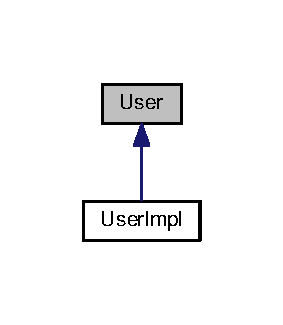
\includegraphics[width=136pt]{dd/de7/classUser__inherit__graph}
\end{center}
\end{figure}
\subsection*{Public Member Functions}
\begin{DoxyCompactItemize}
\item 
virtual Q\+String \hyperlink{classUser_ae468e9100cfb4ab518863393d3d15bbd}{get\+Username} ()=0
\begin{DoxyCompactList}\small\item\em Consulta o nome do usuário. \end{DoxyCompactList}\item 
virtual void \hyperlink{classUser_af026df21b06a8cab417707cbce3a4f8b}{set\+Username} (Q\+String username)=0
\begin{DoxyCompactList}\small\item\em Altera o nome do usuário. \end{DoxyCompactList}\item 
virtual Q\+String \hyperlink{classUser_a552814f109b3892d39e1d43a411bb89e}{get\+Password} ()=0
\begin{DoxyCompactList}\small\item\em Consulta a senha do usuário. \end{DoxyCompactList}\item 
virtual void \hyperlink{classUser_a4bcb0c01280d285d35efe7bfc35c1641}{set\+Password} (Q\+String password)=0
\begin{DoxyCompactList}\small\item\em Altera o nome do usuário. \end{DoxyCompactList}\item 
virtual void \hyperlink{classUser_a0a41c08c3c4a4b5fc778fc3137fd6a8c}{add\+Role} (\hyperlink{classRole}{Role} $\ast$role)=0
\begin{DoxyCompactList}\small\item\em Adiciona um novo papel ao usuário, caso ele já não tenha essa atribuição. \end{DoxyCompactList}\item 
virtual \hyperlink{classRole}{Role} $\ast$ \hyperlink{classUser_a4a67b5285f21c7f33e9efe4326f608e4}{as\+Role} (Q\+String name)=0
\begin{DoxyCompactList}\small\item\em Retorna o papel correspondente ao name solicitado. \end{DoxyCompactList}\end{DoxyCompactItemize}


\subsection{Detailed Description}
Interface correspondente a qualquer usuário do sistema. 

\subsection{Member Function Documentation}
\index{User@{User}!add\+Role@{add\+Role}}
\index{add\+Role@{add\+Role}!User@{User}}
\subsubsection[{\texorpdfstring{add\+Role(\+Role $\ast$role)=0}{addRole(Role *role)=0}}]{\setlength{\rightskip}{0pt plus 5cm}virtual void User\+::add\+Role (
\begin{DoxyParamCaption}
\item[{{\bf Role} $\ast$}]{role}
\end{DoxyParamCaption}
)\hspace{0.3cm}{\ttfamily [pure virtual]}}\hypertarget{classUser_a0a41c08c3c4a4b5fc778fc3137fd6a8c}{}\label{classUser_a0a41c08c3c4a4b5fc778fc3137fd6a8c}


Adiciona um novo papel ao usuário, caso ele já não tenha essa atribuição. 


\begin{DoxyParams}{Parameters}
{\em role} & Novo papel do usuário \\
\hline
\end{DoxyParams}


Implemented in \hyperlink{classUserImpl_a80b1ee2caff4b1ae1c67076096f1acf5}{User\+Impl}.

\index{User@{User}!as\+Role@{as\+Role}}
\index{as\+Role@{as\+Role}!User@{User}}
\subsubsection[{\texorpdfstring{as\+Role(\+Q\+String name)=0}{asRole(QString name)=0}}]{\setlength{\rightskip}{0pt plus 5cm}virtual {\bf Role}$\ast$ User\+::as\+Role (
\begin{DoxyParamCaption}
\item[{Q\+String}]{name}
\end{DoxyParamCaption}
)\hspace{0.3cm}{\ttfamily [pure virtual]}}\hypertarget{classUser_a4a67b5285f21c7f33e9efe4326f608e4}{}\label{classUser_a4a67b5285f21c7f33e9efe4326f608e4}


Retorna o papel correspondente ao name solicitado. 


\begin{DoxyParams}{Parameters}
{\em name} & Nome do papel \\
\hline
\end{DoxyParams}
\begin{DoxyReturn}{Returns}
Papel correspondente 
\end{DoxyReturn}


Implemented in \hyperlink{classUserImpl_a7ee6cdd620e02d565b78f1655aa1b980}{User\+Impl}.

\index{User@{User}!get\+Password@{get\+Password}}
\index{get\+Password@{get\+Password}!User@{User}}
\subsubsection[{\texorpdfstring{get\+Password()=0}{getPassword()=0}}]{\setlength{\rightskip}{0pt plus 5cm}virtual Q\+String User\+::get\+Password (
\begin{DoxyParamCaption}
{}
\end{DoxyParamCaption}
)\hspace{0.3cm}{\ttfamily [pure virtual]}}\hypertarget{classUser_a552814f109b3892d39e1d43a411bb89e}{}\label{classUser_a552814f109b3892d39e1d43a411bb89e}


Consulta a senha do usuário. 

\begin{DoxyReturn}{Returns}
Senha do usuário 
\end{DoxyReturn}


Implemented in \hyperlink{classUserImpl_a38f1527c6ca0b75401bddd68858050bd}{User\+Impl}.

\index{User@{User}!get\+Username@{get\+Username}}
\index{get\+Username@{get\+Username}!User@{User}}
\subsubsection[{\texorpdfstring{get\+Username()=0}{getUsername()=0}}]{\setlength{\rightskip}{0pt plus 5cm}virtual Q\+String User\+::get\+Username (
\begin{DoxyParamCaption}
{}
\end{DoxyParamCaption}
)\hspace{0.3cm}{\ttfamily [pure virtual]}}\hypertarget{classUser_ae468e9100cfb4ab518863393d3d15bbd}{}\label{classUser_ae468e9100cfb4ab518863393d3d15bbd}


Consulta o nome do usuário. 

\begin{DoxyReturn}{Returns}
Nome do usuário 
\end{DoxyReturn}


Implemented in \hyperlink{classUserImpl_abefec7a8158c1304813d0304cf28d79f}{User\+Impl}.

\index{User@{User}!set\+Password@{set\+Password}}
\index{set\+Password@{set\+Password}!User@{User}}
\subsubsection[{\texorpdfstring{set\+Password(\+Q\+String password)=0}{setPassword(QString password)=0}}]{\setlength{\rightskip}{0pt plus 5cm}virtual void User\+::set\+Password (
\begin{DoxyParamCaption}
\item[{Q\+String}]{password}
\end{DoxyParamCaption}
)\hspace{0.3cm}{\ttfamily [pure virtual]}}\hypertarget{classUser_a4bcb0c01280d285d35efe7bfc35c1641}{}\label{classUser_a4bcb0c01280d285d35efe7bfc35c1641}


Altera o nome do usuário. 


\begin{DoxyParams}{Parameters}
{\em password} & Senha do usuário \\
\hline
\end{DoxyParams}


Implemented in \hyperlink{classUserImpl_ae25b0e053e4a3f6b6d4ddf601cb9d7d1}{User\+Impl}.

\index{User@{User}!set\+Username@{set\+Username}}
\index{set\+Username@{set\+Username}!User@{User}}
\subsubsection[{\texorpdfstring{set\+Username(\+Q\+String username)=0}{setUsername(QString username)=0}}]{\setlength{\rightskip}{0pt plus 5cm}virtual void User\+::set\+Username (
\begin{DoxyParamCaption}
\item[{Q\+String}]{username}
\end{DoxyParamCaption}
)\hspace{0.3cm}{\ttfamily [pure virtual]}}\hypertarget{classUser_af026df21b06a8cab417707cbce3a4f8b}{}\label{classUser_af026df21b06a8cab417707cbce3a4f8b}


Altera o nome do usuário. 


\begin{DoxyParams}{Parameters}
{\em username} & Nome do usuário \\
\hline
\end{DoxyParams}


Implemented in \hyperlink{classUserImpl_aeaf34ca2e23f1a673a6997cae77f7452}{User\+Impl}.



The documentation for this class was generated from the following file\+:\begin{DoxyCompactItemize}
\item 
Calc\+Client/src/data/\hyperlink{user_8h}{user.\+h}\end{DoxyCompactItemize}

\hypertarget{classUserImpl}{}\section{User\+Impl Class Reference}
\label{classUserImpl}\index{User\+Impl@{User\+Impl}}


Implementação da interface \hyperlink{classUser}{User}.  




{\ttfamily \#include $<$userimpl.\+h$>$}



Inheritance diagram for User\+Impl\+:
\nopagebreak
\begin{figure}[H]
\begin{center}
\leavevmode
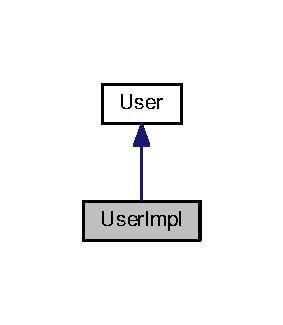
\includegraphics[width=136pt]{db/da3/classUserImpl__inherit__graph}
\end{center}
\end{figure}


Collaboration diagram for User\+Impl\+:
\nopagebreak
\begin{figure}[H]
\begin{center}
\leavevmode
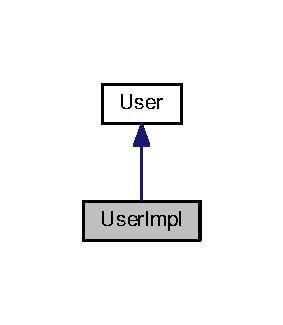
\includegraphics[width=136pt]{df/d98/classUserImpl__coll__graph}
\end{center}
\end{figure}
\subsection*{Public Member Functions}
\begin{DoxyCompactItemize}
\item 
\hyperlink{classUserImpl_a247633b3d3fb9449719bd9c12873b4cb}{User\+Impl} ()\hypertarget{classUserImpl_a247633b3d3fb9449719bd9c12873b4cb}{}\label{classUserImpl_a247633b3d3fb9449719bd9c12873b4cb}

\begin{DoxyCompactList}\small\item\em Construtor padrão. \end{DoxyCompactList}\item 
virtual Q\+String \hyperlink{classUserImpl_abefec7a8158c1304813d0304cf28d79f}{get\+Username} () override
\begin{DoxyCompactList}\small\item\em Consulta o nome do usuário. \end{DoxyCompactList}\item 
virtual void \hyperlink{classUserImpl_aeaf34ca2e23f1a673a6997cae77f7452}{set\+Username} (Q\+String \hyperlink{classUserImpl_aa4cc87da6bbd23b8a3c88dabbe3026f3}{username}) override
\begin{DoxyCompactList}\small\item\em Altera o nome do usuário. \end{DoxyCompactList}\item 
virtual Q\+String \hyperlink{classUserImpl_a38f1527c6ca0b75401bddd68858050bd}{get\+Password} () override
\begin{DoxyCompactList}\small\item\em Consulta a senha do usuário. \end{DoxyCompactList}\item 
virtual void \hyperlink{classUserImpl_ae25b0e053e4a3f6b6d4ddf601cb9d7d1}{set\+Password} (Q\+String \hyperlink{classUserImpl_a4213f64d517183df08c5dab39398bbd0}{password}) override
\begin{DoxyCompactList}\small\item\em Altera o nome do usuário. \end{DoxyCompactList}\item 
virtual void \hyperlink{classUserImpl_a80b1ee2caff4b1ae1c67076096f1acf5}{add\+Role} (\hyperlink{classRole}{Role} $\ast$role) override
\begin{DoxyCompactList}\small\item\em Adiciona um novo papel ao usuário, caso ele já não tenha essa atribuição. \end{DoxyCompactList}\item 
virtual \hyperlink{classRole}{Role} $\ast$ \hyperlink{classUserImpl_a7ee6cdd620e02d565b78f1655aa1b980}{as\+Role} (Q\+String name) override
\begin{DoxyCompactList}\small\item\em Retorna o papel correspondente ao name solicitado. \end{DoxyCompactList}\end{DoxyCompactItemize}
\subsection*{Private Attributes}
\begin{DoxyCompactItemize}
\item 
Q\+String \hyperlink{classUserImpl_aa4cc87da6bbd23b8a3c88dabbe3026f3}{username}\hypertarget{classUserImpl_aa4cc87da6bbd23b8a3c88dabbe3026f3}{}\label{classUserImpl_aa4cc87da6bbd23b8a3c88dabbe3026f3}

\begin{DoxyCompactList}\small\item\em Nome do usuário. \end{DoxyCompactList}\item 
Q\+String \hyperlink{classUserImpl_a4213f64d517183df08c5dab39398bbd0}{password}\hypertarget{classUserImpl_a4213f64d517183df08c5dab39398bbd0}{}\label{classUserImpl_a4213f64d517183df08c5dab39398bbd0}

\begin{DoxyCompactList}\small\item\em Senha do usuário. \end{DoxyCompactList}\item 
vector$<$ \hyperlink{classRole}{Role} $\ast$ $>$ \hyperlink{classUserImpl_a4656b5507c8b8d9975145e954e4641be}{roles}\hypertarget{classUserImpl_a4656b5507c8b8d9975145e954e4641be}{}\label{classUserImpl_a4656b5507c8b8d9975145e954e4641be}

\begin{DoxyCompactList}\small\item\em Array contendo os papeis do usuário. \end{DoxyCompactList}\end{DoxyCompactItemize}


\subsection{Detailed Description}
Implementação da interface \hyperlink{classUser}{User}. 

\subsection{Member Function Documentation}
\index{User\+Impl@{User\+Impl}!add\+Role@{add\+Role}}
\index{add\+Role@{add\+Role}!User\+Impl@{User\+Impl}}
\subsubsection[{\texorpdfstring{add\+Role(\+Role $\ast$role) override}{addRole(Role *role) override}}]{\setlength{\rightskip}{0pt plus 5cm}void User\+Impl\+::add\+Role (
\begin{DoxyParamCaption}
\item[{{\bf Role} $\ast$}]{role}
\end{DoxyParamCaption}
)\hspace{0.3cm}{\ttfamily [override]}, {\ttfamily [virtual]}}\hypertarget{classUserImpl_a80b1ee2caff4b1ae1c67076096f1acf5}{}\label{classUserImpl_a80b1ee2caff4b1ae1c67076096f1acf5}


Adiciona um novo papel ao usuário, caso ele já não tenha essa atribuição. 


\begin{DoxyParams}{Parameters}
{\em role} & Novo papel do usuário \\
\hline
\end{DoxyParams}


Implements \hyperlink{classUser_a0a41c08c3c4a4b5fc778fc3137fd6a8c}{User}.

\index{User\+Impl@{User\+Impl}!as\+Role@{as\+Role}}
\index{as\+Role@{as\+Role}!User\+Impl@{User\+Impl}}
\subsubsection[{\texorpdfstring{as\+Role(\+Q\+String name) override}{asRole(QString name) override}}]{\setlength{\rightskip}{0pt plus 5cm}{\bf Role} $\ast$ User\+Impl\+::as\+Role (
\begin{DoxyParamCaption}
\item[{Q\+String}]{name}
\end{DoxyParamCaption}
)\hspace{0.3cm}{\ttfamily [override]}, {\ttfamily [virtual]}}\hypertarget{classUserImpl_a7ee6cdd620e02d565b78f1655aa1b980}{}\label{classUserImpl_a7ee6cdd620e02d565b78f1655aa1b980}


Retorna o papel correspondente ao name solicitado. 


\begin{DoxyParams}{Parameters}
{\em name} & Nome do papel \\
\hline
\end{DoxyParams}
\begin{DoxyReturn}{Returns}
Papel correspondente 
\end{DoxyReturn}


Implements \hyperlink{classUser_a4a67b5285f21c7f33e9efe4326f608e4}{User}.

\index{User\+Impl@{User\+Impl}!get\+Password@{get\+Password}}
\index{get\+Password@{get\+Password}!User\+Impl@{User\+Impl}}
\subsubsection[{\texorpdfstring{get\+Password() override}{getPassword() override}}]{\setlength{\rightskip}{0pt plus 5cm}Q\+String User\+Impl\+::get\+Password (
\begin{DoxyParamCaption}
{}
\end{DoxyParamCaption}
)\hspace{0.3cm}{\ttfamily [override]}, {\ttfamily [virtual]}}\hypertarget{classUserImpl_a38f1527c6ca0b75401bddd68858050bd}{}\label{classUserImpl_a38f1527c6ca0b75401bddd68858050bd}


Consulta a senha do usuário. 

\begin{DoxyReturn}{Returns}
Senha do usuário 
\end{DoxyReturn}


Implements \hyperlink{classUser_a552814f109b3892d39e1d43a411bb89e}{User}.

\index{User\+Impl@{User\+Impl}!get\+Username@{get\+Username}}
\index{get\+Username@{get\+Username}!User\+Impl@{User\+Impl}}
\subsubsection[{\texorpdfstring{get\+Username() override}{getUsername() override}}]{\setlength{\rightskip}{0pt plus 5cm}Q\+String User\+Impl\+::get\+Username (
\begin{DoxyParamCaption}
{}
\end{DoxyParamCaption}
)\hspace{0.3cm}{\ttfamily [override]}, {\ttfamily [virtual]}}\hypertarget{classUserImpl_abefec7a8158c1304813d0304cf28d79f}{}\label{classUserImpl_abefec7a8158c1304813d0304cf28d79f}


Consulta o nome do usuário. 

\begin{DoxyReturn}{Returns}
Nome do usuário 
\end{DoxyReturn}


Implements \hyperlink{classUser_ae468e9100cfb4ab518863393d3d15bbd}{User}.

\index{User\+Impl@{User\+Impl}!set\+Password@{set\+Password}}
\index{set\+Password@{set\+Password}!User\+Impl@{User\+Impl}}
\subsubsection[{\texorpdfstring{set\+Password(\+Q\+String password) override}{setPassword(QString password) override}}]{\setlength{\rightskip}{0pt plus 5cm}void User\+Impl\+::set\+Password (
\begin{DoxyParamCaption}
\item[{Q\+String}]{password}
\end{DoxyParamCaption}
)\hspace{0.3cm}{\ttfamily [override]}, {\ttfamily [virtual]}}\hypertarget{classUserImpl_ae25b0e053e4a3f6b6d4ddf601cb9d7d1}{}\label{classUserImpl_ae25b0e053e4a3f6b6d4ddf601cb9d7d1}


Altera o nome do usuário. 


\begin{DoxyParams}{Parameters}
{\em password} & Senha do usuário \\
\hline
\end{DoxyParams}


Implements \hyperlink{classUser_a4bcb0c01280d285d35efe7bfc35c1641}{User}.

\index{User\+Impl@{User\+Impl}!set\+Username@{set\+Username}}
\index{set\+Username@{set\+Username}!User\+Impl@{User\+Impl}}
\subsubsection[{\texorpdfstring{set\+Username(\+Q\+String username) override}{setUsername(QString username) override}}]{\setlength{\rightskip}{0pt plus 5cm}void User\+Impl\+::set\+Username (
\begin{DoxyParamCaption}
\item[{Q\+String}]{username}
\end{DoxyParamCaption}
)\hspace{0.3cm}{\ttfamily [override]}, {\ttfamily [virtual]}}\hypertarget{classUserImpl_aeaf34ca2e23f1a673a6997cae77f7452}{}\label{classUserImpl_aeaf34ca2e23f1a673a6997cae77f7452}


Altera o nome do usuário. 


\begin{DoxyParams}{Parameters}
{\em username} & Nome do usuário \\
\hline
\end{DoxyParams}


Implements \hyperlink{classUser_af026df21b06a8cab417707cbce3a4f8b}{User}.



The documentation for this class was generated from the following files\+:\begin{DoxyCompactItemize}
\item 
Calc\+Client/src/data/\hyperlink{userimpl_8h}{userimpl.\+h}\item 
Calc\+Client/src/data/\hyperlink{userimpl_8cpp}{userimpl.\+cpp}\end{DoxyCompactItemize}

\hypertarget{classWorkerThread}{}\section{Worker\+Thread Class Reference}
\label{classWorkerThread}\index{Worker\+Thread@{Worker\+Thread}}


Interface para thread de trabalho auxiliar.  




{\ttfamily \#include $<$workerthread.\+h$>$}



Inheritance diagram for Worker\+Thread\+:\nopagebreak
\begin{figure}[H]
\begin{center}
\leavevmode
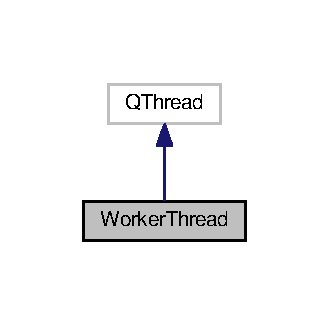
\includegraphics[width=177pt]{d3/da8/classWorkerThread__inherit__graph}
\end{center}
\end{figure}
\subsection*{Public Member Functions}
\begin{DoxyCompactItemize}
\item 
virtual void \hyperlink{classWorkerThread_a008dd6f762a2c20641afbb2a69319ca4}{run} ()=0
\begin{DoxyCompactList}\small\item\em Método para delegação do tratamento de uma mensagem recebida e envio da respostas. \end{DoxyCompactList}\item 
virtual void \hyperlink{classWorkerThread_a4d6d532dfbb27c5a435018ea697acb11}{start} ()=0\hypertarget{classWorkerThread_a4d6d532dfbb27c5a435018ea697acb11}{}\label{classWorkerThread_a4d6d532dfbb27c5a435018ea697acb11}

\begin{DoxyCompactList}\small\item\em Método para o inicio de execução de uma \hyperlink{classWorkerThread}{Worker\+Thread}. \end{DoxyCompactList}\item 
virtual void \hyperlink{classWorkerThread_a270d44343c31516acebd9544788e3886}{finished} ()=0\hypertarget{classWorkerThread_a270d44343c31516acebd9544788e3886}{}\label{classWorkerThread_a270d44343c31516acebd9544788e3886}

\begin{DoxyCompactList}\small\item\em Representa o fim de execução de \hyperlink{classWorkerThread}{Worker\+Thread}. \end{DoxyCompactList}\item 
virtual void \hyperlink{classWorkerThread_abf55cfb94dd10a2a3b2ff3896473c11b}{delete\+Later} ()=0\hypertarget{classWorkerThread_abf55cfb94dd10a2a3b2ff3896473c11b}{}\label{classWorkerThread_abf55cfb94dd10a2a3b2ff3896473c11b}

\begin{DoxyCompactList}\small\item\em Responsavel por desalocar elementos da \hyperlink{classWorkerThread}{Worker\+Thread}. \end{DoxyCompactList}\item 
virtual Q\+Object $\ast$ \hyperlink{classWorkerThread_a7cce841d4e0b98ebdeb0c7027045dfc4}{get\+Q\+Object} ()=0
\begin{DoxyCompactList}\small\item\em Método retorna uma referência a um objeto Q\+Object correspondente a essa classe. \end{DoxyCompactList}\end{DoxyCompactItemize}


\subsection{Detailed Description}
Interface para thread de trabalho auxiliar. 

\subsection{Member Function Documentation}
\index{Worker\+Thread@{Worker\+Thread}!get\+Q\+Object@{get\+Q\+Object}}
\index{get\+Q\+Object@{get\+Q\+Object}!Worker\+Thread@{Worker\+Thread}}
\subsubsection[{\texorpdfstring{get\+Q\+Object()=0}{getQObject()=0}}]{\setlength{\rightskip}{0pt plus 5cm}virtual Q\+Object$\ast$ Worker\+Thread\+::get\+Q\+Object (
\begin{DoxyParamCaption}
{}
\end{DoxyParamCaption}
)\hspace{0.3cm}{\ttfamily [pure virtual]}}\hypertarget{classWorkerThread_a7cce841d4e0b98ebdeb0c7027045dfc4}{}\label{classWorkerThread_a7cce841d4e0b98ebdeb0c7027045dfc4}


Método retorna uma referência a um objeto Q\+Object correspondente a essa classe. 

\begin{DoxyReturn}{Returns}
Referencia ao Q\+Object correspondente a classe. 
\end{DoxyReturn}


Implemented in \hyperlink{classWorkerThreadImpl_a30689eaffcb664bc95644bf497ea1446}{Worker\+Thread\+Impl}.

\index{Worker\+Thread@{Worker\+Thread}!run@{run}}
\index{run@{run}!Worker\+Thread@{Worker\+Thread}}
\subsubsection[{\texorpdfstring{run()=0}{run()=0}}]{\setlength{\rightskip}{0pt plus 5cm}virtual void Worker\+Thread\+::run (
\begin{DoxyParamCaption}
{}
\end{DoxyParamCaption}
)\hspace{0.3cm}{\ttfamily [pure virtual]}}\hypertarget{classWorkerThread_a008dd6f762a2c20641afbb2a69319ca4}{}\label{classWorkerThread_a008dd6f762a2c20641afbb2a69319ca4}


Método para delegação do tratamento de uma mensagem recebida e envio da respostas. 

Este método recebe um byte array correspondente a um objeto J\+S\+ON, após isso cria um objeto J\+S\+ON e delega a resolução da mensagem para o método handl\+Message. Por fim, recebe a resposta da mensagem, codifica ela e envia ao cliente pela rede.

\begin{DoxySeeAlso}{See also}
\hyperlink{classWorkerThreadImpl_ac1ced60fd043f7dca8a7e7e1857a91cb}{Worker\+Thread\+Impl\+::handle\+Message(\+Q\+Json\+Object)}, \hyperlink{classWorkerThreadImpl_ae260562530b71dc55a6d360d5e4d896d}{Worker\+Thread\+Impl\+::error(\+Q\+Tcp\+Socket\+::\+Socket\+Error)}. 
\end{DoxySeeAlso}


Implemented in \hyperlink{classWorkerThreadImpl_a24ef315ed0b7914ffd099c23a5a6e16c}{Worker\+Thread\+Impl}.



The documentation for this class was generated from the following file\+:\begin{DoxyCompactItemize}
\item 
Calc\+Server/\hyperlink{workerthread_8h}{workerthread.\+h}\end{DoxyCompactItemize}

\hypertarget{classWorkerThreadImpl}{}\section{Worker\+Thread\+Impl Class Reference}
\label{classWorkerThreadImpl}\index{Worker\+Thread\+Impl@{Worker\+Thread\+Impl}}


Implementação da interface \hyperlink{classWorkerThread}{Worker\+Thread} para realização de operações do servidor em uma thread.  




{\ttfamily \#include $<$workerthreadimpl.\+h$>$}



Inheritance diagram for Worker\+Thread\+Impl\+:\nopagebreak
\begin{figure}[H]
\begin{center}
\leavevmode
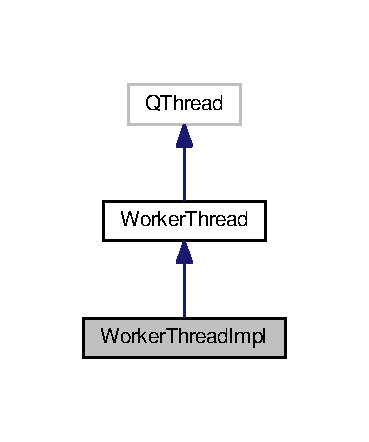
\includegraphics[width=230pt]{d6/d44/classWorkerThreadImpl__inherit__graph}
\end{center}
\end{figure}


Collaboration diagram for Worker\+Thread\+Impl\+:\nopagebreak
\begin{figure}[H]
\begin{center}
\leavevmode
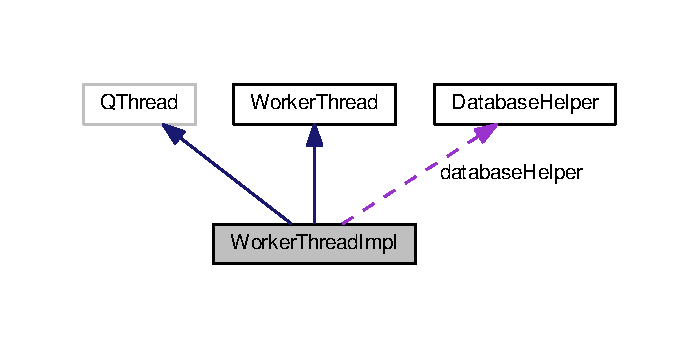
\includegraphics[width=336pt]{de/d29/classWorkerThreadImpl__coll__graph}
\end{center}
\end{figure}
\subsection*{Signals}
\begin{DoxyCompactItemize}
\item 
void \hyperlink{classWorkerThreadImpl_ae260562530b71dc55a6d360d5e4d896d}{error} (Q\+Tcp\+Socket\+::\+Socket\+Error socket\+Error)
\begin{DoxyCompactList}\small\item\em Signal utilizado para sinalizar erros. \end{DoxyCompactList}\item 
virtual void \hyperlink{classWorkerThreadImpl_aca36cb83741dce52b5d92cc7a2844257}{finished} () override
\begin{DoxyCompactList}\small\item\em Representa o fim de execução de \hyperlink{classWorkerThreadImpl}{Worker\+Thread\+Impl}. \end{DoxyCompactList}\end{DoxyCompactItemize}
\subsection*{Public Member Functions}
\begin{DoxyCompactItemize}
\item 
\hyperlink{classWorkerThreadImpl_a61d57c319668cbf86ad1642e8471b6db}{Worker\+Thread\+Impl} (qintptr \hyperlink{classWorkerThreadImpl_af3d6cf4437a92a4dbdf8c07a474a671b}{socket\+Descriptor}, Q\+Object $\ast$parent, \hyperlink{classDatabaseHelper}{Database\+Helper} $\ast$\hyperlink{classWorkerThreadImpl_a6a64f8daf91e56abf94c5a92bfc0fb88}{database\+Helper})
\begin{DoxyCompactList}\small\item\em Construtor para configurar a thread. \end{DoxyCompactList}\item 
virtual \hyperlink{classWorkerThreadImpl_acdb8da302c73c5ab454445029bbe6da1}{$\sim$\+Worker\+Thread\+Impl} () override\hypertarget{classWorkerThreadImpl_acdb8da302c73c5ab454445029bbe6da1}{}\label{classWorkerThreadImpl_acdb8da302c73c5ab454445029bbe6da1}

\begin{DoxyCompactList}\small\item\em Destrutor Padrão. \end{DoxyCompactList}\item 
virtual void \hyperlink{classWorkerThreadImpl_a24ef315ed0b7914ffd099c23a5a6e16c}{run} () override
\begin{DoxyCompactList}\small\item\em Método para delegação do tratamento de uma mensagem recebida e envio da respostas. \end{DoxyCompactList}\item 
virtual void \hyperlink{classWorkerThreadImpl_a16a04e1fd50d1bcb425e70a3ac219786}{start} () override
\begin{DoxyCompactList}\small\item\em Método para o inicio de execução de uma \hyperlink{classWorkerThread}{Worker\+Thread}. \end{DoxyCompactList}\item 
virtual void \hyperlink{classWorkerThreadImpl_a0c7acd90839e238ff12eba997132f532}{delete\+Later} () override\hypertarget{classWorkerThreadImpl_a0c7acd90839e238ff12eba997132f532}{}\label{classWorkerThreadImpl_a0c7acd90839e238ff12eba997132f532}

\begin{DoxyCompactList}\small\item\em Responsavel por desalocar elementos da \hyperlink{classWorkerThread}{Worker\+Thread}. \end{DoxyCompactList}\item 
virtual Q\+Object $\ast$ \hyperlink{classWorkerThreadImpl_a30689eaffcb664bc95644bf497ea1446}{get\+Q\+Object} () override
\begin{DoxyCompactList}\small\item\em Método retorna uma referência a um objeto Q\+Object correspondente a essa classe. \end{DoxyCompactList}\end{DoxyCompactItemize}
\subsection*{Protected Attributes}
\begin{DoxyCompactItemize}
\item 
qintptr \hyperlink{classWorkerThreadImpl_af3d6cf4437a92a4dbdf8c07a474a671b}{socket\+Descriptor}\hypertarget{classWorkerThreadImpl_af3d6cf4437a92a4dbdf8c07a474a671b}{}\label{classWorkerThreadImpl_af3d6cf4437a92a4dbdf8c07a474a671b}

\begin{DoxyCompactList}\small\item\em Contém as informações de configuração do socket. \end{DoxyCompactList}\item 
\hyperlink{classDatabaseHelper}{Database\+Helper} $\ast$ \hyperlink{classWorkerThreadImpl_a6a64f8daf91e56abf94c5a92bfc0fb88}{database\+Helper}\hypertarget{classWorkerThreadImpl_a6a64f8daf91e56abf94c5a92bfc0fb88}{}\label{classWorkerThreadImpl_a6a64f8daf91e56abf94c5a92bfc0fb88}

\begin{DoxyCompactList}\small\item\em Referência ao helper de acesso ao banco de dados. \end{DoxyCompactList}\end{DoxyCompactItemize}
\subsection*{Private Member Functions}
\begin{DoxyCompactItemize}
\item 
\hyperlink{classWorkerThreadImpl_adebf1655473918cb3ff77fbac14ca7d3}{Worker\+Thread\+Impl} (const \hyperlink{classWorkerThreadImpl}{Worker\+Thread\+Impl} \&rhs)
\begin{DoxyCompactList}\small\item\em Construtor de Cópia. \end{DoxyCompactList}\item 
\hyperlink{classWorkerThreadImpl}{Worker\+Thread\+Impl} \& \hyperlink{classWorkerThreadImpl_a20a17134c17a8832fe6a59220d801dd0}{operator=} (const \hyperlink{classWorkerThreadImpl}{Worker\+Thread\+Impl} \&rhs)
\begin{DoxyCompactList}\small\item\em Sobrecarga do operador =. \end{DoxyCompactList}\item 
\hyperlink{classWorkerThreadImpl_a6656b99702598782c9c49ee9e4437388}{Worker\+Thread\+Impl} ()
\begin{DoxyCompactList}\small\item\em Construtor Padrão. \end{DoxyCompactList}\item 
Q\+Json\+Object \hyperlink{classWorkerThreadImpl_ac1ced60fd043f7dca8a7e7e1857a91cb}{handle\+Message} (Q\+Json\+Object json\+Object)
\begin{DoxyCompactList}\small\item\em Rotina auxiliar para o tratamento de mensagens recebidas. \end{DoxyCompactList}\item 
Q\+Json\+Object \hyperlink{classWorkerThreadImpl_a72b7f275f170171a49725a508e071f71}{handle\+Authenticate} (Q\+Json\+Object json\+Object)
\begin{DoxyCompactList}\small\item\em Método para tratamento de mensagens de autenticação. \end{DoxyCompactList}\item 
Q\+Json\+Object \hyperlink{classWorkerThreadImpl_a0bcd0f706b49530ccaf7f3fc21bded7c}{handle\+Operation} (Q\+Json\+Object json\+Object)
\begin{DoxyCompactList}\small\item\em Método para realizar uma operação e armazena-\/la em banco. \end{DoxyCompactList}\item 
Q\+Json\+Object \hyperlink{classWorkerThreadImpl_a9ce30db393c61dd414d198b1dcb38ddb}{handle\+User\+Report} (Q\+Json\+Object json\+Object)
\begin{DoxyCompactList}\small\item\em Método gera um relatório de operações do usuário informado. \end{DoxyCompactList}\item 
Q\+Json\+Object \hyperlink{classWorkerThreadImpl_a31f8bcb7340bc4a2497d12e5bbf4c203}{handle\+All\+Users\+Report} (Q\+Json\+Object json\+Object)
\begin{DoxyCompactList}\small\item\em Método gera um relatório de operações de todos usuários. \end{DoxyCompactList}\end{DoxyCompactItemize}
\subsection*{Friends}
\begin{DoxyCompactItemize}
\item 
class \hyperlink{classWorkerThreadImpl_a9b782f47c630bd470969aeba01a706b2}{Operacoes\+Test}\hypertarget{classWorkerThreadImpl_a9b782f47c630bd470969aeba01a706b2}{}\label{classWorkerThreadImpl_a9b782f47c630bd470969aeba01a706b2}

\begin{DoxyCompactList}\small\item\em Classe de Testes para \hyperlink{classWorkerThread}{Worker\+Thread}. \end{DoxyCompactList}\end{DoxyCompactItemize}


\subsection{Detailed Description}
Implementação da interface \hyperlink{classWorkerThread}{Worker\+Thread} para realização de operações do servidor em uma thread. 

\subsection{Constructor \& Destructor Documentation}
\index{Worker\+Thread\+Impl@{Worker\+Thread\+Impl}!Worker\+Thread\+Impl@{Worker\+Thread\+Impl}}
\index{Worker\+Thread\+Impl@{Worker\+Thread\+Impl}!Worker\+Thread\+Impl@{Worker\+Thread\+Impl}}
\subsubsection[{\texorpdfstring{Worker\+Thread\+Impl(qintptr socket\+Descriptor, Q\+Object $\ast$parent, Database\+Helper $\ast$database\+Helper)}{WorkerThreadImpl(qintptr socketDescriptor, QObject *parent, DatabaseHelper *databaseHelper)}}]{\setlength{\rightskip}{0pt plus 5cm}Worker\+Thread\+Impl\+::\+Worker\+Thread\+Impl (
\begin{DoxyParamCaption}
\item[{qintptr}]{socket\+Descriptor, }
\item[{Q\+Object $\ast$}]{parent, }
\item[{{\bf Database\+Helper} $\ast$}]{database\+Helper}
\end{DoxyParamCaption}
)}\hypertarget{classWorkerThreadImpl_a61d57c319668cbf86ad1642e8471b6db}{}\label{classWorkerThreadImpl_a61d57c319668cbf86ad1642e8471b6db}


Construtor para configurar a thread. 

Ao ser chamado este construtor seta os atributos para os valores informados.


\begin{DoxyParams}{Parameters}
{\em socket\+Descriptor} & Informações de configuração do socket. \\
\hline
{\em parent} & Referência ao componente pai. \\
\hline
{\em database\+Helper} & Referência ao helper de acesso ao banco de dados.\\
\hline
\end{DoxyParams}
\begin{DoxySeeAlso}{See also}
\hyperlink{classWorkerThreadImpl_a6656b99702598782c9c49ee9e4437388}{Worker\+Thread\+Impl\+::\+Worker\+Thread\+Impl()}. 
\end{DoxySeeAlso}
\index{Worker\+Thread\+Impl@{Worker\+Thread\+Impl}!Worker\+Thread\+Impl@{Worker\+Thread\+Impl}}
\index{Worker\+Thread\+Impl@{Worker\+Thread\+Impl}!Worker\+Thread\+Impl@{Worker\+Thread\+Impl}}
\subsubsection[{\texorpdfstring{Worker\+Thread\+Impl(const Worker\+Thread\+Impl \&rhs)}{WorkerThreadImpl(const WorkerThreadImpl &rhs)}}]{\setlength{\rightskip}{0pt plus 5cm}Worker\+Thread\+Impl\+::\+Worker\+Thread\+Impl (
\begin{DoxyParamCaption}
\item[{const {\bf Worker\+Thread\+Impl} \&}]{rhs}
\end{DoxyParamCaption}
)\hspace{0.3cm}{\ttfamily [private]}}\hypertarget{classWorkerThreadImpl_adebf1655473918cb3ff77fbac14ca7d3}{}\label{classWorkerThreadImpl_adebf1655473918cb3ff77fbac14ca7d3}


Construtor de Cópia. 


\begin{DoxyParams}{Parameters}
{\em rhs} & Objeto a ser copiado. \\
\hline
\end{DoxyParams}
\index{Worker\+Thread\+Impl@{Worker\+Thread\+Impl}!Worker\+Thread\+Impl@{Worker\+Thread\+Impl}}
\index{Worker\+Thread\+Impl@{Worker\+Thread\+Impl}!Worker\+Thread\+Impl@{Worker\+Thread\+Impl}}
\subsubsection[{\texorpdfstring{Worker\+Thread\+Impl()}{WorkerThreadImpl()}}]{\setlength{\rightskip}{0pt plus 5cm}Worker\+Thread\+Impl\+::\+Worker\+Thread\+Impl (
\begin{DoxyParamCaption}
{}
\end{DoxyParamCaption}
)\hspace{0.3cm}{\ttfamily [private]}}\hypertarget{classWorkerThreadImpl_a6656b99702598782c9c49ee9e4437388}{}\label{classWorkerThreadImpl_a6656b99702598782c9c49ee9e4437388}


Construtor Padrão. 

\begin{DoxySeeAlso}{See also}
\hyperlink{classWorkerThreadImpl_a61d57c319668cbf86ad1642e8471b6db}{Worker\+Thread\+Impl\+::\+Worker\+Thread\+Impl(qintptr, Q\+Object$\ast$, Database\+Helper$\ast$)} 
\end{DoxySeeAlso}


\subsection{Member Function Documentation}
\index{Worker\+Thread\+Impl@{Worker\+Thread\+Impl}!error@{error}}
\index{error@{error}!Worker\+Thread\+Impl@{Worker\+Thread\+Impl}}
\subsubsection[{\texorpdfstring{error}{error}}]{\setlength{\rightskip}{0pt plus 5cm}void Worker\+Thread\+Impl\+::error (
\begin{DoxyParamCaption}
\item[{Q\+Tcp\+Socket\+::\+Socket\+Error}]{socket\+Error}
\end{DoxyParamCaption}
)\hspace{0.3cm}{\ttfamily [signal]}}\hypertarget{classWorkerThreadImpl_ae260562530b71dc55a6d360d5e4d896d}{}\label{classWorkerThreadImpl_ae260562530b71dc55a6d360d5e4d896d}


Signal utilizado para sinalizar erros. 


\begin{DoxyParams}{Parameters}
{\em socket\+Error} & Tipo do erro detectado. \\
\hline
\end{DoxyParams}
\index{Worker\+Thread\+Impl@{Worker\+Thread\+Impl}!finished@{finished}}
\index{finished@{finished}!Worker\+Thread\+Impl@{Worker\+Thread\+Impl}}
\subsubsection[{\texorpdfstring{finished}{finished}}]{\setlength{\rightskip}{0pt plus 5cm}virtual void Worker\+Thread\+Impl\+::finished (
\begin{DoxyParamCaption}
{}
\end{DoxyParamCaption}
)\hspace{0.3cm}{\ttfamily [override]}, {\ttfamily [virtual]}, {\ttfamily [signal]}}\hypertarget{classWorkerThreadImpl_aca36cb83741dce52b5d92cc7a2844257}{}\label{classWorkerThreadImpl_aca36cb83741dce52b5d92cc7a2844257}


Representa o fim de execução de \hyperlink{classWorkerThreadImpl}{Worker\+Thread\+Impl}. 

\begin{DoxySeeAlso}{See also}
\hyperlink{classWorkerThread_a270d44343c31516acebd9544788e3886}{Worker\+Thread\+::finished()}. 
\end{DoxySeeAlso}
\index{Worker\+Thread\+Impl@{Worker\+Thread\+Impl}!get\+Q\+Object@{get\+Q\+Object}}
\index{get\+Q\+Object@{get\+Q\+Object}!Worker\+Thread\+Impl@{Worker\+Thread\+Impl}}
\subsubsection[{\texorpdfstring{get\+Q\+Object() override}{getQObject() override}}]{\setlength{\rightskip}{0pt plus 5cm}Q\+Object $\ast$ Worker\+Thread\+Impl\+::get\+Q\+Object (
\begin{DoxyParamCaption}
{}
\end{DoxyParamCaption}
)\hspace{0.3cm}{\ttfamily [override]}, {\ttfamily [virtual]}}\hypertarget{classWorkerThreadImpl_a30689eaffcb664bc95644bf497ea1446}{}\label{classWorkerThreadImpl_a30689eaffcb664bc95644bf497ea1446}


Método retorna uma referência a um objeto Q\+Object correspondente a essa classe. 

\begin{DoxyReturn}{Returns}
Referencia ao Q\+Object correspondente a classe. 
\end{DoxyReturn}


Implements \hyperlink{classWorkerThread_a7cce841d4e0b98ebdeb0c7027045dfc4}{Worker\+Thread}.

\index{Worker\+Thread\+Impl@{Worker\+Thread\+Impl}!handle\+All\+Users\+Report@{handle\+All\+Users\+Report}}
\index{handle\+All\+Users\+Report@{handle\+All\+Users\+Report}!Worker\+Thread\+Impl@{Worker\+Thread\+Impl}}
\subsubsection[{\texorpdfstring{handle\+All\+Users\+Report(\+Q\+Json\+Object json\+Object)}{handleAllUsersReport(QJsonObject jsonObject)}}]{\setlength{\rightskip}{0pt plus 5cm}Q\+Json\+Object Worker\+Thread\+Impl\+::handle\+All\+Users\+Report (
\begin{DoxyParamCaption}
\item[{Q\+Json\+Object}]{json\+Object}
\end{DoxyParamCaption}
)\hspace{0.3cm}{\ttfamily [private]}}\hypertarget{classWorkerThreadImpl_a31f8bcb7340bc4a2497d12e5bbf4c203}{}\label{classWorkerThreadImpl_a31f8bcb7340bc4a2497d12e5bbf4c203}


Método gera um relatório de operações de todos usuários. 

Este método recebe um J\+S\+ON contendo os dados necessário. Ao extrair o nome do usuário, verifica se ele é administrador, portanto se tem autorização para realizar essa operação. Sendo verdadeiro, ele realiza uma agregação no banco para obter a quantidade de operações de todos os usuários.


\begin{DoxyParams}{Parameters}
{\em json\+Object} & Dados da mensagem recebida. \\
\hline
\end{DoxyParams}
\begin{DoxyReturn}{Returns}
Dados codificado em um mensagem de resposta.
\end{DoxyReturn}
\begin{DoxySeeAlso}{See also}
\hyperlink{classWorkerThreadImpl_ac1ced60fd043f7dca8a7e7e1857a91cb}{Worker\+Thread\+Impl\+::handle\+Message(\+Q\+Json\+Object)} 
\end{DoxySeeAlso}
\index{Worker\+Thread\+Impl@{Worker\+Thread\+Impl}!handle\+Authenticate@{handle\+Authenticate}}
\index{handle\+Authenticate@{handle\+Authenticate}!Worker\+Thread\+Impl@{Worker\+Thread\+Impl}}
\subsubsection[{\texorpdfstring{handle\+Authenticate(\+Q\+Json\+Object json\+Object)}{handleAuthenticate(QJsonObject jsonObject)}}]{\setlength{\rightskip}{0pt plus 5cm}Q\+Json\+Object Worker\+Thread\+Impl\+::handle\+Authenticate (
\begin{DoxyParamCaption}
\item[{Q\+Json\+Object}]{json\+Object}
\end{DoxyParamCaption}
)\hspace{0.3cm}{\ttfamily [private]}}\hypertarget{classWorkerThreadImpl_a72b7f275f170171a49725a508e071f71}{}\label{classWorkerThreadImpl_a72b7f275f170171a49725a508e071f71}


Método para tratamento de mensagens de autenticação. 

O método recebe um objeto J\+S\+ON contendo as informações de login de um usuário, extrai esses dados e verifica se eles estão armazenados no banco, caso positivo responde que é um usuário valido e verifica se ele é um administrador, caso negativo responde que o usuário é invalido.


\begin{DoxyParams}{Parameters}
{\em json\+Object} & Dados da mensagem recebida. \\
\hline
\end{DoxyParams}
\begin{DoxyReturn}{Returns}
Dados codificado em um mensagem de resposta.
\end{DoxyReturn}
\begin{DoxySeeAlso}{See also}
\hyperlink{classWorkerThreadImpl_ac1ced60fd043f7dca8a7e7e1857a91cb}{Worker\+Thread\+Impl\+::handle\+Message(\+Q\+Json\+Object)} 
\end{DoxySeeAlso}
\index{Worker\+Thread\+Impl@{Worker\+Thread\+Impl}!handle\+Message@{handle\+Message}}
\index{handle\+Message@{handle\+Message}!Worker\+Thread\+Impl@{Worker\+Thread\+Impl}}
\subsubsection[{\texorpdfstring{handle\+Message(\+Q\+Json\+Object json\+Object)}{handleMessage(QJsonObject jsonObject)}}]{\setlength{\rightskip}{0pt plus 5cm}Q\+Json\+Object Worker\+Thread\+Impl\+::handle\+Message (
\begin{DoxyParamCaption}
\item[{Q\+Json\+Object}]{json\+Object}
\end{DoxyParamCaption}
)\hspace{0.3cm}{\ttfamily [private]}}\hypertarget{classWorkerThreadImpl_ac1ced60fd043f7dca8a7e7e1857a91cb}{}\label{classWorkerThreadImpl_ac1ced60fd043f7dca8a7e7e1857a91cb}


Rotina auxiliar para o tratamento de mensagens recebidas. 

O método recebe uma mensagem J\+S\+ON, extrai o tipo de mensagem dos dados contidos no J\+S\+ON e delega o tratamento dos dados restantes para alguns dos métodos handle disponiveis.


\begin{DoxyParams}{Parameters}
{\em json\+Object} & Dados da mensagem recebida. \\
\hline
\end{DoxyParams}
\begin{DoxyReturn}{Returns}
Dados codificado em um mensagem de resposta.
\end{DoxyReturn}
\begin{DoxySeeAlso}{See also}
\hyperlink{classWorkerThreadImpl_a72b7f275f170171a49725a508e071f71}{Worker\+Thread\+Impl\+::handle\+Authenticate(\+Q\+Json\+Object)}, \hyperlink{classWorkerThreadImpl_a0bcd0f706b49530ccaf7f3fc21bded7c}{Worker\+Thread\+Impl\+::handle\+Operation(\+Q\+Json\+Object)}, \hyperlink{classWorkerThreadImpl_a9ce30db393c61dd414d198b1dcb38ddb}{Worker\+Thread\+Impl\+::handle\+User\+Report(\+Q\+Json\+Object)}, \hyperlink{classWorkerThreadImpl_a31f8bcb7340bc4a2497d12e5bbf4c203}{Worker\+Thread\+Impl\+::handle\+All\+Users\+Report(\+Q\+Json\+Object)}. 
\end{DoxySeeAlso}
\index{Worker\+Thread\+Impl@{Worker\+Thread\+Impl}!handle\+Operation@{handle\+Operation}}
\index{handle\+Operation@{handle\+Operation}!Worker\+Thread\+Impl@{Worker\+Thread\+Impl}}
\subsubsection[{\texorpdfstring{handle\+Operation(\+Q\+Json\+Object json\+Object)}{handleOperation(QJsonObject jsonObject)}}]{\setlength{\rightskip}{0pt plus 5cm}Q\+Json\+Object Worker\+Thread\+Impl\+::handle\+Operation (
\begin{DoxyParamCaption}
\item[{Q\+Json\+Object}]{json\+Object}
\end{DoxyParamCaption}
)\hspace{0.3cm}{\ttfamily [private]}}\hypertarget{classWorkerThreadImpl_a0bcd0f706b49530ccaf7f3fc21bded7c}{}\label{classWorkerThreadImpl_a0bcd0f706b49530ccaf7f3fc21bded7c}


Método para realizar uma operação e armazena-\/la em banco. 

O método recebe um objeto J\+S\+ON contendo as informações da operação a ser realizada. Sendo assim, ele extrai os dados do J\+S\+ON e realiza a operação, após isso armazena o registro no banco e responde o usuário com a solução da operação.


\begin{DoxyParams}{Parameters}
{\em json\+Object} & Dados da mensagem recebida. \\
\hline
\end{DoxyParams}
\begin{DoxyReturn}{Returns}
Dados codificado em um mensagem de resposta.
\end{DoxyReturn}
\begin{DoxySeeAlso}{See also}
\hyperlink{classWorkerThreadImpl_ac1ced60fd043f7dca8a7e7e1857a91cb}{Worker\+Thread\+Impl\+::handle\+Message(\+Q\+Json\+Object)} 
\end{DoxySeeAlso}
\index{Worker\+Thread\+Impl@{Worker\+Thread\+Impl}!handle\+User\+Report@{handle\+User\+Report}}
\index{handle\+User\+Report@{handle\+User\+Report}!Worker\+Thread\+Impl@{Worker\+Thread\+Impl}}
\subsubsection[{\texorpdfstring{handle\+User\+Report(\+Q\+Json\+Object json\+Object)}{handleUserReport(QJsonObject jsonObject)}}]{\setlength{\rightskip}{0pt plus 5cm}Q\+Json\+Object Worker\+Thread\+Impl\+::handle\+User\+Report (
\begin{DoxyParamCaption}
\item[{Q\+Json\+Object}]{json\+Object}
\end{DoxyParamCaption}
)\hspace{0.3cm}{\ttfamily [private]}}\hypertarget{classWorkerThreadImpl_a9ce30db393c61dd414d198b1dcb38ddb}{}\label{classWorkerThreadImpl_a9ce30db393c61dd414d198b1dcb38ddb}


Método gera um relatório de operações do usuário informado. 

Este método recebe um J\+S\+ON contendo os dados necessário. Ao extrair o nome do usuário, ele realiza uma agregação no banco para obter a quantidade de operações que o usuário informado realizou.


\begin{DoxyParams}{Parameters}
{\em json\+Object} & Dados da mensagem recebida. \\
\hline
\end{DoxyParams}
\begin{DoxyReturn}{Returns}
Dados codificado em um mensagem de resposta.
\end{DoxyReturn}
\begin{DoxySeeAlso}{See also}
\hyperlink{classWorkerThreadImpl_ac1ced60fd043f7dca8a7e7e1857a91cb}{Worker\+Thread\+Impl\+::handle\+Message(\+Q\+Json\+Object)} 
\end{DoxySeeAlso}
\index{Worker\+Thread\+Impl@{Worker\+Thread\+Impl}!operator=@{operator=}}
\index{operator=@{operator=}!Worker\+Thread\+Impl@{Worker\+Thread\+Impl}}
\subsubsection[{\texorpdfstring{operator=(const Worker\+Thread\+Impl \&rhs)}{operator=(const WorkerThreadImpl &rhs)}}]{\setlength{\rightskip}{0pt plus 5cm}{\bf Worker\+Thread\+Impl} \& Worker\+Thread\+Impl\+::operator= (
\begin{DoxyParamCaption}
\item[{const {\bf Worker\+Thread\+Impl} \&}]{rhs}
\end{DoxyParamCaption}
)\hspace{0.3cm}{\ttfamily [private]}}\hypertarget{classWorkerThreadImpl_a20a17134c17a8832fe6a59220d801dd0}{}\label{classWorkerThreadImpl_a20a17134c17a8832fe6a59220d801dd0}


Sobrecarga do operador =. 


\begin{DoxyParams}{Parameters}
{\em rhs} & Objeto a ser copiado. \\
\hline
\end{DoxyParams}
\begin{DoxyReturn}{Returns}
Novo objeto copiado. 
\end{DoxyReturn}
\index{Worker\+Thread\+Impl@{Worker\+Thread\+Impl}!run@{run}}
\index{run@{run}!Worker\+Thread\+Impl@{Worker\+Thread\+Impl}}
\subsubsection[{\texorpdfstring{run() override}{run() override}}]{\setlength{\rightskip}{0pt plus 5cm}void Worker\+Thread\+Impl\+::run (
\begin{DoxyParamCaption}
{}
\end{DoxyParamCaption}
)\hspace{0.3cm}{\ttfamily [override]}, {\ttfamily [virtual]}}\hypertarget{classWorkerThreadImpl_a24ef315ed0b7914ffd099c23a5a6e16c}{}\label{classWorkerThreadImpl_a24ef315ed0b7914ffd099c23a5a6e16c}


Método para delegação do tratamento de uma mensagem recebida e envio da respostas. 

Este método recebe um byte array correspondente a um objeto J\+S\+ON, após isso cria um objeto J\+S\+ON e delega a resolução da mensagem para o método handl\+Message. Por fim, recebe a resposta da mensagem, codifica ela e envia ao cliente pela rede.

\begin{DoxySeeAlso}{See also}
\hyperlink{classWorkerThreadImpl_ac1ced60fd043f7dca8a7e7e1857a91cb}{Worker\+Thread\+Impl\+::handle\+Message(\+Q\+Json\+Object)}, \hyperlink{classWorkerThreadImpl_ae260562530b71dc55a6d360d5e4d896d}{Worker\+Thread\+Impl\+::error(\+Q\+Tcp\+Socket\+::\+Socket\+Error)}. 
\end{DoxySeeAlso}


Implements \hyperlink{classWorkerThread_a008dd6f762a2c20641afbb2a69319ca4}{Worker\+Thread}.

\index{Worker\+Thread\+Impl@{Worker\+Thread\+Impl}!start@{start}}
\index{start@{start}!Worker\+Thread\+Impl@{Worker\+Thread\+Impl}}
\subsubsection[{\texorpdfstring{start() override}{start() override}}]{\setlength{\rightskip}{0pt plus 5cm}void Worker\+Thread\+Impl\+::start (
\begin{DoxyParamCaption}
{}
\end{DoxyParamCaption}
)\hspace{0.3cm}{\ttfamily [override]}, {\ttfamily [virtual]}}\hypertarget{classWorkerThreadImpl_a16a04e1fd50d1bcb425e70a3ac219786}{}\label{classWorkerThreadImpl_a16a04e1fd50d1bcb425e70a3ac219786}


Método para o inicio de execução de uma \hyperlink{classWorkerThread}{Worker\+Thread}. 

\begin{DoxySeeAlso}{See also}
\hyperlink{classWorkerThreadImpl_aca36cb83741dce52b5d92cc7a2844257}{Worker\+Thread\+Impl\+::finished()}. 
\end{DoxySeeAlso}


Implements \hyperlink{classWorkerThread_a4d6d532dfbb27c5a435018ea697acb11}{Worker\+Thread}.



The documentation for this class was generated from the following files\+:\begin{DoxyCompactItemize}
\item 
Calc\+Server/\hyperlink{workerthreadimpl_8h}{workerthreadimpl.\+h}\item 
Calc\+Server/\hyperlink{workerthreadimpl_8cpp}{workerthreadimpl.\+cpp}\end{DoxyCompactItemize}

\chapter{File Documentation}
\hypertarget{networkmanager_8h}{}\section{Calc\+Client/src/control/networkmanager.h File Reference}
\label{networkmanager_8h}\index{Calc\+Client/src/control/networkmanager.\+h@{Calc\+Client/src/control/networkmanager.\+h}}
{\ttfamily \#include $<$Q\+String$>$}\\*
{\ttfamily \#include $<$Q\+Object$>$}\\*
{\ttfamily \#include $<$Q\+Json\+Object$>$}\\*
{\ttfamily \#include $<$data/adminuser.\+h$>$}\\*
{\ttfamily \#include $<$data/basicuser.\+h$>$}\\*
Include dependency graph for networkmanager.\+h\+:
\nopagebreak
\begin{figure}[H]
\begin{center}
\leavevmode
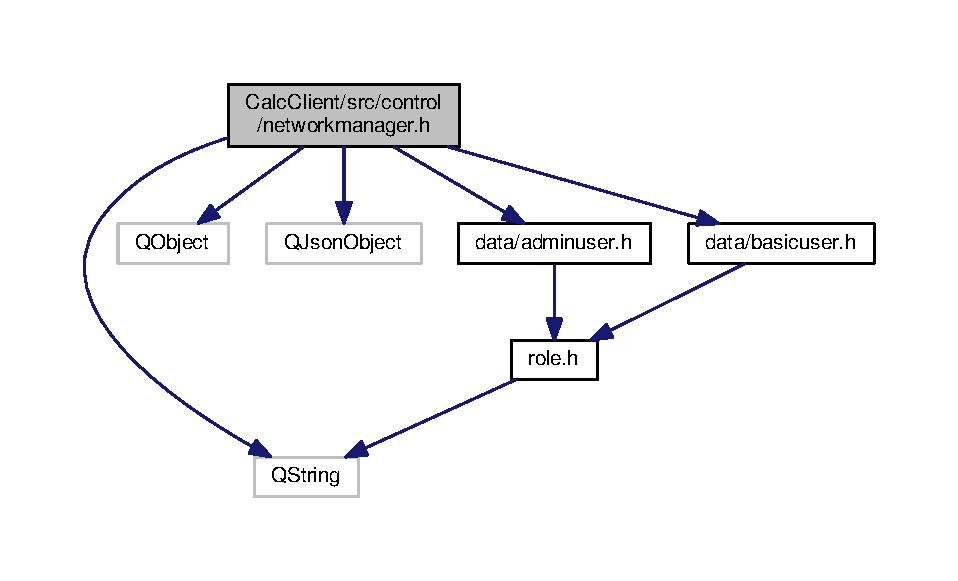
\includegraphics[width=350pt]{d1/d5d/networkmanager_8h__incl}
\end{center}
\end{figure}
This graph shows which files directly or indirectly include this file\+:
\nopagebreak
\begin{figure}[H]
\begin{center}
\leavevmode
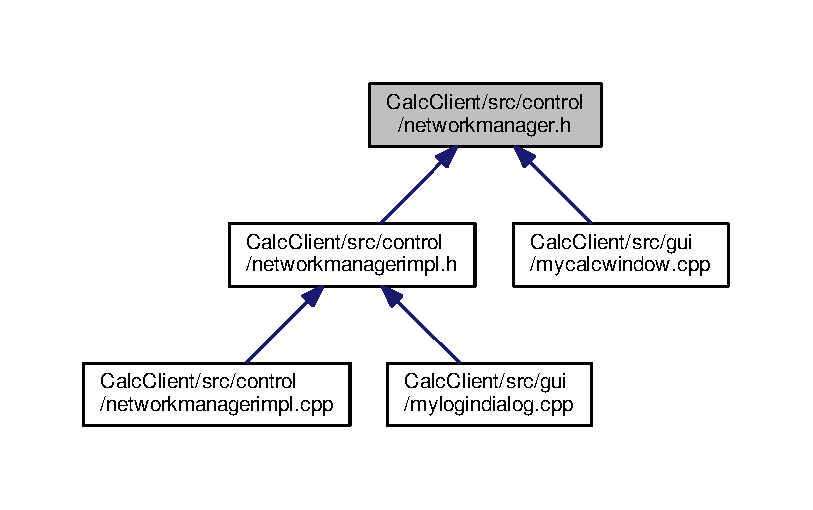
\includegraphics[width=350pt]{da/d43/networkmanager_8h__dep__incl}
\end{center}
\end{figure}
\subsection*{Classes}
\begin{DoxyCompactItemize}
\item 
class \hyperlink{classNetworkManager}{Network\+Manager}
\begin{DoxyCompactList}\small\item\em Classe para gerenciar comunicações entre a gui e o server pela rede. \end{DoxyCompactList}\end{DoxyCompactItemize}


\subsection{Detailed Description}
Arquivo contendo a Declaração da Interface \hyperlink{classNetworkManager}{Network\+Manager} 
\hypertarget{networkmanagerimpl_8cpp}{}\section{Calc\+Client/src/control/networkmanagerimpl.cpp File Reference}
\label{networkmanagerimpl_8cpp}\index{Calc\+Client/src/control/networkmanagerimpl.\+cpp@{Calc\+Client/src/control/networkmanagerimpl.\+cpp}}
{\ttfamily \#include \char`\"{}networkmanagerimpl.\+h\char`\"{}}\\*
{\ttfamily \#include $<$Q\+Json\+Document$>$}\\*
Include dependency graph for networkmanagerimpl.\+cpp\+:
\nopagebreak
\begin{figure}[H]
\begin{center}
\leavevmode
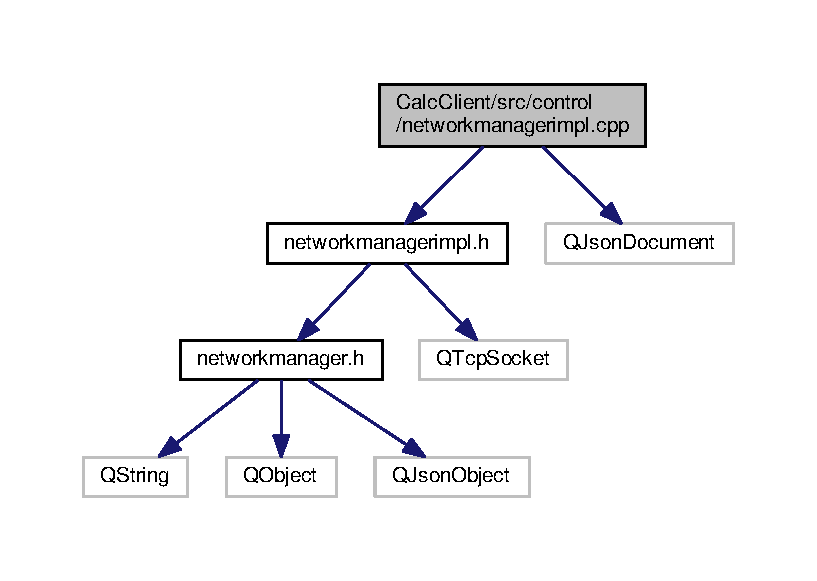
\includegraphics[width=350pt]{d6/d08/networkmanagerimpl_8cpp__incl}
\end{center}
\end{figure}


\subsection{Detailed Description}
Arquivo contendo a Implementação da Classe \hyperlink{classNetworkManagerImpl}{Network\+Manager\+Impl} 
\hypertarget{networkmanagerimpl_8h}{}\section{Calc\+Client/src/control/networkmanagerimpl.h File Reference}
\label{networkmanagerimpl_8h}\index{Calc\+Client/src/control/networkmanagerimpl.\+h@{Calc\+Client/src/control/networkmanagerimpl.\+h}}
{\ttfamily \#include \char`\"{}networkmanager.\+h\char`\"{}}\\*
{\ttfamily \#include $<$Q\+Tcp\+Socket$>$}\\*
Include dependency graph for networkmanagerimpl.\+h\+:
\nopagebreak
\begin{figure}[H]
\begin{center}
\leavevmode
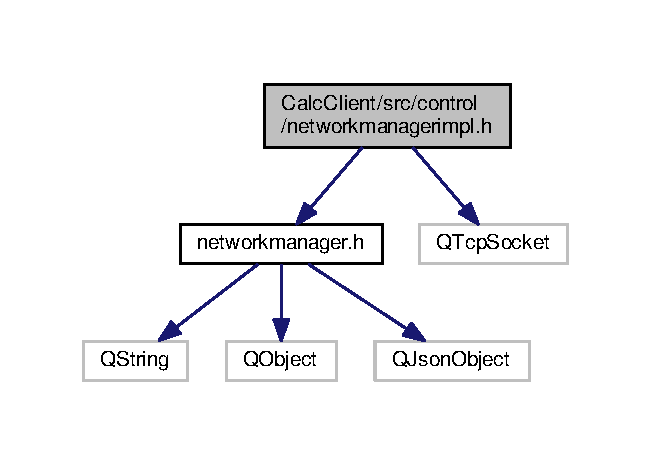
\includegraphics[width=350pt]{d5/de9/networkmanagerimpl_8h__incl}
\end{center}
\end{figure}
This graph shows which files directly or indirectly include this file\+:
\nopagebreak
\begin{figure}[H]
\begin{center}
\leavevmode
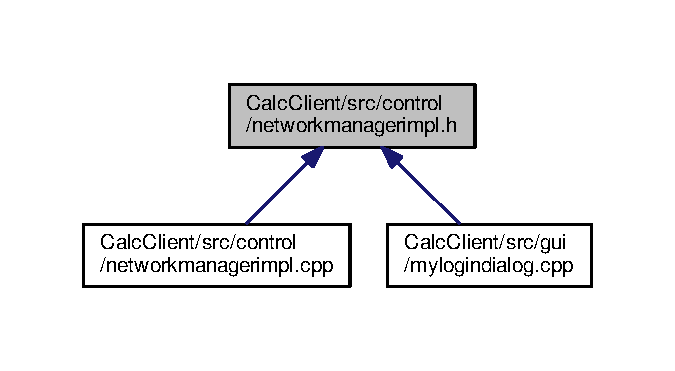
\includegraphics[width=324pt]{df/dbf/networkmanagerimpl_8h__dep__incl}
\end{center}
\end{figure}
\subsection*{Classes}
\begin{DoxyCompactItemize}
\item 
class \hyperlink{classNetworkManagerImpl}{Network\+Manager\+Impl}
\begin{DoxyCompactList}\small\item\em Implementação da Interface \hyperlink{classNetworkManager}{Network\+Manager}. \end{DoxyCompactList}\end{DoxyCompactItemize}


\subsection{Detailed Description}
Arquivo contendo a Declaração da Classe \hyperlink{classNetworkManagerImpl}{Network\+Manager\+Impl} 
\hypertarget{adminuser_8h}{}\section{Calc\+Client/src/data/adminuser.h File Reference}
\label{adminuser_8h}\index{Calc\+Client/src/data/adminuser.\+h@{Calc\+Client/src/data/adminuser.\+h}}
{\ttfamily \#include \char`\"{}role.\+h\char`\"{}}\\*
Include dependency graph for adminuser.\+h\+:
\nopagebreak
\begin{figure}[H]
\begin{center}
\leavevmode
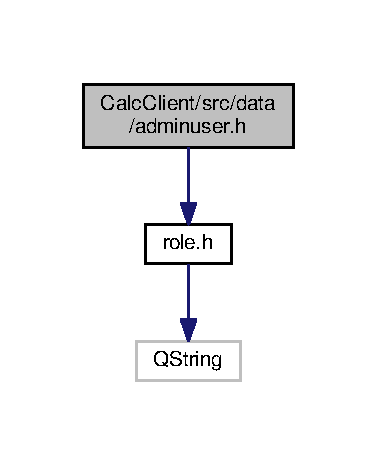
\includegraphics[width=181pt]{da/db8/adminuser_8h__incl}
\end{center}
\end{figure}
This graph shows which files directly or indirectly include this file\+:
\nopagebreak
\begin{figure}[H]
\begin{center}
\leavevmode
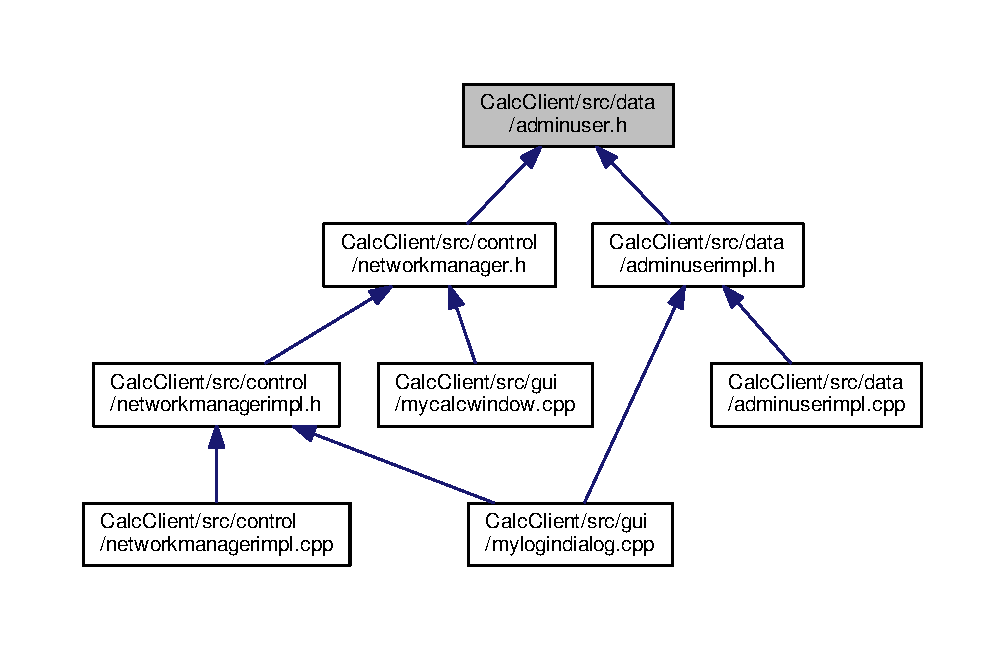
\includegraphics[width=350pt]{d4/d27/adminuser_8h__dep__incl}
\end{center}
\end{figure}
\subsection*{Classes}
\begin{DoxyCompactItemize}
\item 
class \hyperlink{classAdminUser}{Admin\+User}
\begin{DoxyCompactList}\small\item\em Interface correspondente ao papel de administrador do sistema. \end{DoxyCompactList}\end{DoxyCompactItemize}


\subsection{Detailed Description}
Arquivo contendo a Declaração da Interface \hyperlink{classAdminUser}{Admin\+User} 
\hypertarget{adminuserimpl_8cpp}{}\section{Calc\+Client/src/data/adminuserimpl.cpp File Reference}
\label{adminuserimpl_8cpp}\index{Calc\+Client/src/data/adminuserimpl.\+cpp@{Calc\+Client/src/data/adminuserimpl.\+cpp}}
{\ttfamily \#include \char`\"{}adminuserimpl.\+h\char`\"{}}\\*
Include dependency graph for adminuserimpl.\+cpp\+:
\nopagebreak
\begin{figure}[H]
\begin{center}
\leavevmode
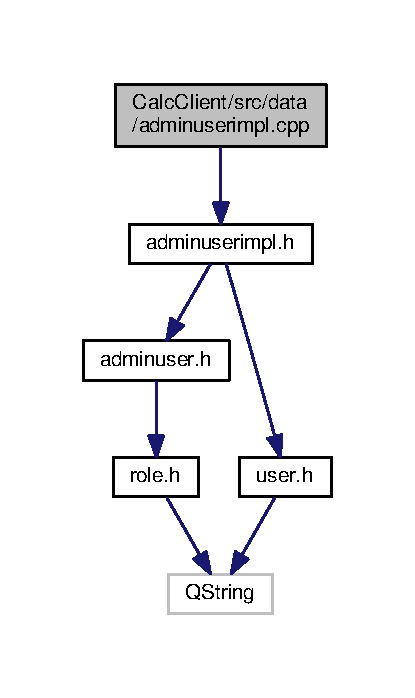
\includegraphics[width=199pt]{de/d7a/adminuserimpl_8cpp__incl}
\end{center}
\end{figure}


\subsection{Detailed Description}
Arquivo contendo a Implementação da Classe \hyperlink{classAdminUserImpl}{Admin\+User\+Impl} 
\hypertarget{adminuserimpl_8h}{}\section{Calc\+Client/src/data/adminuserimpl.h File Reference}
\label{adminuserimpl_8h}\index{Calc\+Client/src/data/adminuserimpl.\+h@{Calc\+Client/src/data/adminuserimpl.\+h}}
{\ttfamily \#include \char`\"{}adminuser.\+h\char`\"{}}\\*
{\ttfamily \#include \char`\"{}user.\+h\char`\"{}}\\*
Include dependency graph for adminuserimpl.\+h\+:
\nopagebreak
\begin{figure}[H]
\begin{center}
\leavevmode
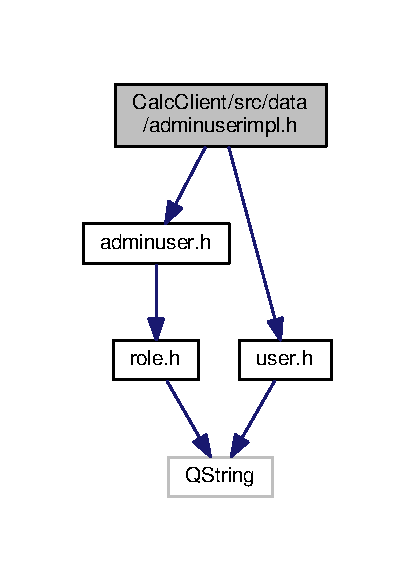
\includegraphics[width=199pt]{df/d0b/adminuserimpl_8h__incl}
\end{center}
\end{figure}
This graph shows which files directly or indirectly include this file\+:
\nopagebreak
\begin{figure}[H]
\begin{center}
\leavevmode
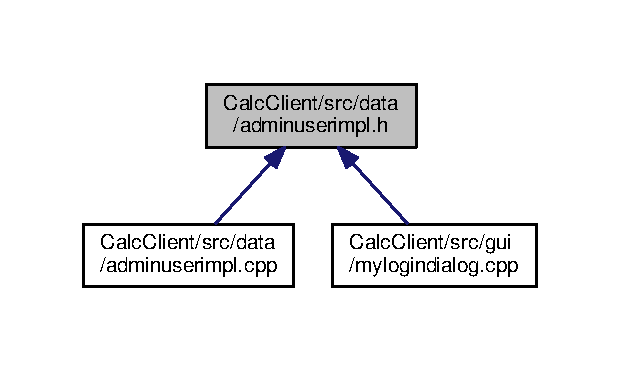
\includegraphics[width=298pt]{d0/dc5/adminuserimpl_8h__dep__incl}
\end{center}
\end{figure}
\subsection*{Classes}
\begin{DoxyCompactItemize}
\item 
class \hyperlink{classAdminUserImpl}{Admin\+User\+Impl}
\begin{DoxyCompactList}\small\item\em Implementação da Interface \hyperlink{classAdminUser}{Admin\+User}. \end{DoxyCompactList}\end{DoxyCompactItemize}


\subsection{Detailed Description}
Arquivo contendo a Declaração da Classe \hyperlink{classAdminUserImpl}{Admin\+User\+Impl} 
\hypertarget{basicuser_8h}{}\section{Calc\+Client/src/data/basicuser.h File Reference}
\label{basicuser_8h}\index{Calc\+Client/src/data/basicuser.\+h@{Calc\+Client/src/data/basicuser.\+h}}
{\ttfamily \#include \char`\"{}role.\+h\char`\"{}}\\*
Include dependency graph for basicuser.\+h\+:
\nopagebreak
\begin{figure}[H]
\begin{center}
\leavevmode
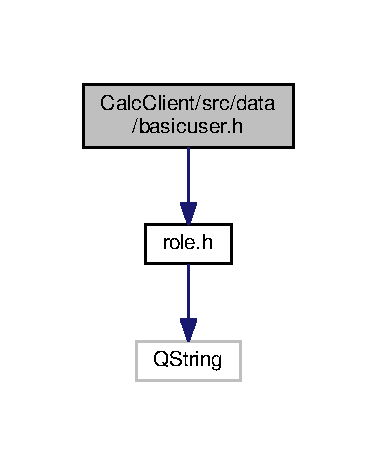
\includegraphics[width=181pt]{db/dde/basicuser_8h__incl}
\end{center}
\end{figure}
This graph shows which files directly or indirectly include this file\+:
\nopagebreak
\begin{figure}[H]
\begin{center}
\leavevmode
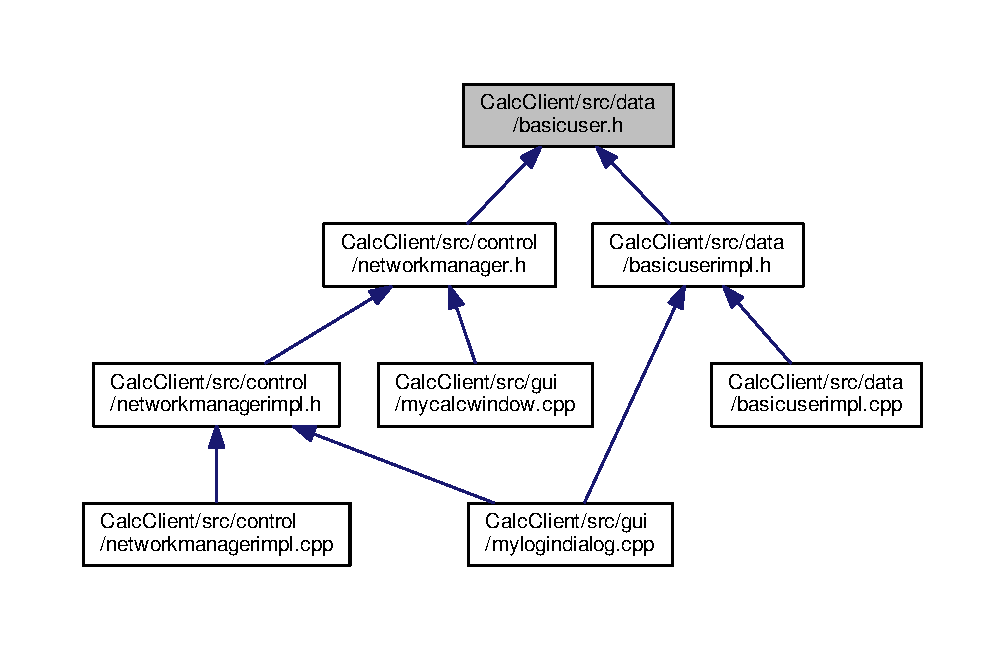
\includegraphics[width=350pt]{d9/dde/basicuser_8h__dep__incl}
\end{center}
\end{figure}
\subsection*{Classes}
\begin{DoxyCompactItemize}
\item 
class \hyperlink{classBasicUser}{Basic\+User}
\begin{DoxyCompactList}\small\item\em Interface correspondente ao papel usuário. \end{DoxyCompactList}\end{DoxyCompactItemize}


\subsection{Detailed Description}
Arquivo contendo a Declaração da Interface \hyperlink{classBasicUser}{Basic\+User} 
\hypertarget{basicuserimpl_8cpp}{}\section{Calc\+Client/src/data/basicuserimpl.cpp File Reference}
\label{basicuserimpl_8cpp}\index{Calc\+Client/src/data/basicuserimpl.\+cpp@{Calc\+Client/src/data/basicuserimpl.\+cpp}}
{\ttfamily \#include \char`\"{}basicuserimpl.\+h\char`\"{}}\\*
Include dependency graph for basicuserimpl.\+cpp\+:
\nopagebreak
\begin{figure}[H]
\begin{center}
\leavevmode
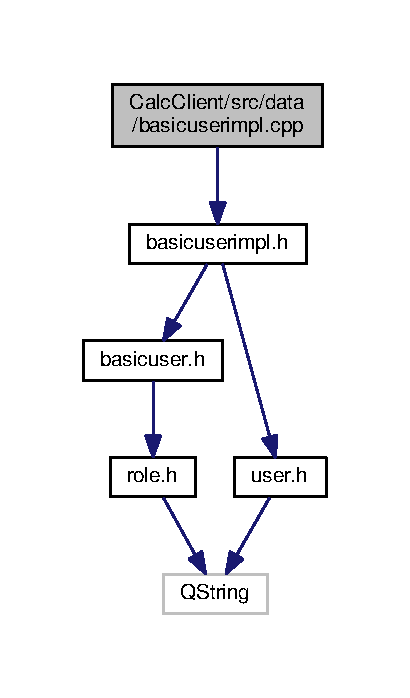
\includegraphics[width=197pt]{d5/dc4/basicuserimpl_8cpp__incl}
\end{center}
\end{figure}


\subsection{Detailed Description}
Arquivo contendo a Implementação da Classe \hyperlink{classBasicUserImpl}{Basic\+User\+Impl} 
\hypertarget{basicuserimpl_8h}{}\section{Calc\+Client/src/data/basicuserimpl.h File Reference}
\label{basicuserimpl_8h}\index{Calc\+Client/src/data/basicuserimpl.\+h@{Calc\+Client/src/data/basicuserimpl.\+h}}
{\ttfamily \#include \char`\"{}basicuser.\+h\char`\"{}}\\*
{\ttfamily \#include \char`\"{}user.\+h\char`\"{}}\\*
Include dependency graph for basicuserimpl.\+h\+:
\nopagebreak
\begin{figure}[H]
\begin{center}
\leavevmode
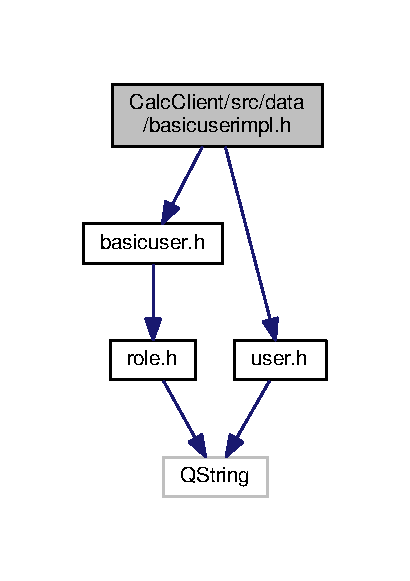
\includegraphics[width=197pt]{de/d9d/basicuserimpl_8h__incl}
\end{center}
\end{figure}
This graph shows which files directly or indirectly include this file\+:
\nopagebreak
\begin{figure}[H]
\begin{center}
\leavevmode
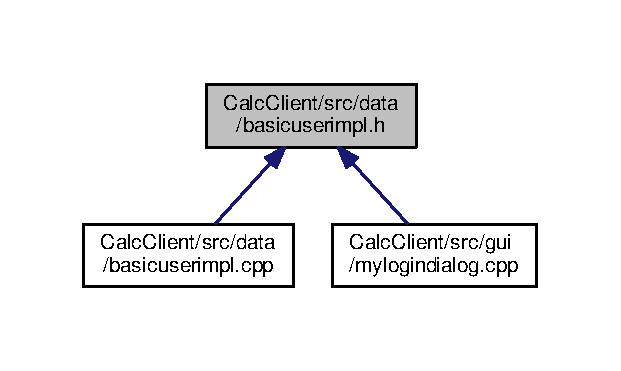
\includegraphics[width=298pt]{d3/dea/basicuserimpl_8h__dep__incl}
\end{center}
\end{figure}
\subsection*{Classes}
\begin{DoxyCompactItemize}
\item 
class \hyperlink{classBasicUserImpl}{Basic\+User\+Impl}
\begin{DoxyCompactList}\small\item\em Implementação da interface \hyperlink{classBasicUser}{Basic\+User}. \end{DoxyCompactList}\end{DoxyCompactItemize}


\subsection{Detailed Description}
Arquivo contendo a Declaração da Classe \hyperlink{classBasicUserImpl}{Basic\+User\+Impl} 
\hypertarget{role_8h}{}\section{Calc\+Client/src/data/role.h File Reference}
\label{role_8h}\index{Calc\+Client/src/data/role.\+h@{Calc\+Client/src/data/role.\+h}}
{\ttfamily \#include $<$Q\+String$>$}\\*
Include dependency graph for role.\+h\+:
\nopagebreak
\begin{figure}[H]
\begin{center}
\leavevmode
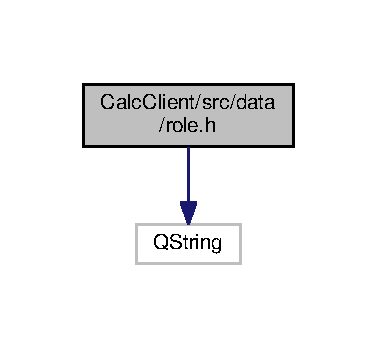
\includegraphics[width=181pt]{d0/d1b/role_8h__incl}
\end{center}
\end{figure}
This graph shows which files directly or indirectly include this file\+:
\nopagebreak
\begin{figure}[H]
\begin{center}
\leavevmode
\includegraphics[width=350pt]{de/d2e/role_8h__dep__incl}
\end{center}
\end{figure}
\subsection*{Classes}
\begin{DoxyCompactItemize}
\item 
class \hyperlink{classRole}{Role}
\begin{DoxyCompactList}\small\item\em Superclasse correspondente aos papeis que podem ser assumidos no sistema. \end{DoxyCompactList}\end{DoxyCompactItemize}


\subsection{Detailed Description}
Arquivo contendo a Declaração da Interface \hyperlink{classRole}{Role} 
\hypertarget{user_8h}{}\section{Calc\+Client/src/data/user.h File Reference}
\label{user_8h}\index{Calc\+Client/src/data/user.\+h@{Calc\+Client/src/data/user.\+h}}
{\ttfamily \#include $<$Q\+String$>$}\\*
Include dependency graph for user.\+h\+:
\nopagebreak
\begin{figure}[H]
\begin{center}
\leavevmode
\includegraphics[width=181pt]{df/dd9/user_8h__incl}
\end{center}
\end{figure}
This graph shows which files directly or indirectly include this file\+:
\nopagebreak
\begin{figure}[H]
\begin{center}
\leavevmode
\includegraphics[width=350pt]{de/de9/user_8h__dep__incl}
\end{center}
\end{figure}
\subsection*{Classes}
\begin{DoxyCompactItemize}
\item 
class \hyperlink{classUser}{User}
\begin{DoxyCompactList}\small\item\em Interface correspondente a qualquer usuário do sistema. \end{DoxyCompactList}\end{DoxyCompactItemize}


\subsection{Detailed Description}
Arquivo contendo a Declaração da Interface \hyperlink{classUser}{User} 
\hypertarget{userimpl_8cpp}{}\section{Calc\+Client/src/data/userimpl.cpp File Reference}
\label{userimpl_8cpp}\index{Calc\+Client/src/data/userimpl.\+cpp@{Calc\+Client/src/data/userimpl.\+cpp}}
{\ttfamily \#include \char`\"{}userimpl.\+h\char`\"{}}\\*
Include dependency graph for userimpl.\+cpp\+:
\nopagebreak
\begin{figure}[H]
\begin{center}
\leavevmode
\includegraphics[width=246pt]{d7/d0c/userimpl_8cpp__incl}
\end{center}
\end{figure}


\subsection{Detailed Description}
Arquivo contendo a Implementação da Classe \hyperlink{classUserImpl}{User\+Impl} 
\hypertarget{userimpl_8h}{}\section{Calc\+Client/src/data/userimpl.h File Reference}
\label{userimpl_8h}\index{Calc\+Client/src/data/userimpl.\+h@{Calc\+Client/src/data/userimpl.\+h}}
{\ttfamily \#include \char`\"{}user.\+h\char`\"{}}\\*
{\ttfamily \#include \char`\"{}role.\+h\char`\"{}}\\*
{\ttfamily \#include $<$vector$>$}\\*
Include dependency graph for userimpl.\+h\+:
\nopagebreak
\begin{figure}[H]
\begin{center}
\leavevmode
\includegraphics[width=246pt]{d6/d73/userimpl_8h__incl}
\end{center}
\end{figure}
This graph shows which files directly or indirectly include this file\+:
\nopagebreak
\begin{figure}[H]
\begin{center}
\leavevmode
\includegraphics[width=298pt]{d8/d9b/userimpl_8h__dep__incl}
\end{center}
\end{figure}
\subsection*{Classes}
\begin{DoxyCompactItemize}
\item 
class \hyperlink{classUserImpl}{User\+Impl}
\begin{DoxyCompactList}\small\item\em Implementação da interface \hyperlink{classUser}{User}. \end{DoxyCompactList}\end{DoxyCompactItemize}


\subsection{Detailed Description}
Arquivo contendo a Declaração da Classe \hyperlink{classUserImpl}{User\+Impl} 
\hypertarget{mycalcwindow_8cpp}{}\section{Calc\+Client/mycalcwindow.cpp File Reference}
\label{mycalcwindow_8cpp}\index{Calc\+Client/mycalcwindow.\+cpp@{Calc\+Client/mycalcwindow.\+cpp}}
{\ttfamily \#include $<$Q\+Sql\+Query$>$}\\*
{\ttfamily \#include $<$Q\+Message\+Box$>$}\\*
{\ttfamily \#include $<$Q\+Debug$>$}\\*
{\ttfamily \#include $<$Q\+Sql\+Error$>$}\\*
{\ttfamily \#include $<$Q\+Json\+Object$>$}\\*
{\ttfamily \#include $<$Q\+Json\+Document$>$}\\*
{\ttfamily \#include $<$string$>$}\\*
{\ttfamily \#include $<$sstream$>$}\\*
{\ttfamily \#include $<$iostream$>$}\\*
{\ttfamily \#include \char`\"{}mycalcwindow.\+h\char`\"{}}\\*
{\ttfamily \#include \char`\"{}ui\+\_\+calcwindow.\+h\char`\"{}}\\*
Include dependency graph for mycalcwindow.\+cpp\+:\nopagebreak
\begin{figure}[H]
\begin{center}
\leavevmode
\includegraphics[width=350pt]{d1/d12/mycalcwindow_8cpp__incl}
\end{center}
\end{figure}
\subsection*{Macros}
\begin{DoxyCompactItemize}
\item 
\#define \hyperlink{mycalcwindow_8cpp_ad72dbcf6d0153db1b8d8a58001feed83}{D\+E\+B\+UG}
\end{DoxyCompactItemize}


\subsection{Detailed Description}
Arquivo contendo a implementação da Classe \hyperlink{classMyCalcWindow}{My\+Calc\+Window}. 

\subsection{Macro Definition Documentation}
\index{mycalcwindow.\+cpp@{mycalcwindow.\+cpp}!D\+E\+B\+UG@{D\+E\+B\+UG}}
\index{D\+E\+B\+UG@{D\+E\+B\+UG}!mycalcwindow.\+cpp@{mycalcwindow.\+cpp}}
\subsubsection[{\texorpdfstring{D\+E\+B\+UG}{DEBUG}}]{\setlength{\rightskip}{0pt plus 5cm}\#define D\+E\+B\+UG}\hypertarget{mycalcwindow_8cpp_ad72dbcf6d0153db1b8d8a58001feed83}{}\label{mycalcwindow_8cpp_ad72dbcf6d0153db1b8d8a58001feed83}
Flag demarcando se as mensagens de debug devem ou não serem exibidas. 
\hypertarget{mycalcwindow_8h}{}\section{Calc\+Client/src/gui/mycalcwindow.h File Reference}
\label{mycalcwindow_8h}\index{Calc\+Client/src/gui/mycalcwindow.\+h@{Calc\+Client/src/gui/mycalcwindow.\+h}}
{\ttfamily \#include $<$Q\+Main\+Window$>$}\\*
{\ttfamily \#include $<$Q\+Tcp\+Socket$>$}\\*
{\ttfamily \#include $<$Qt\+Charts/\+Q\+Chart\+View$>$}\\*
{\ttfamily \#include $<$Qt\+Charts/\+Q\+Pie\+Series$>$}\\*
{\ttfamily \#include $<$Qt\+Charts/\+Q\+Pie\+Slice$>$}\\*
{\ttfamily \#include $<$Q\+Json\+Object$>$}\\*
{\ttfamily \#include $<$utility$>$}\\*
{\ttfamily \#include $<$vector$>$}\\*
{\ttfamily \#include \char`\"{}ui\+\_\+calcwindow.\+h\char`\"{}}\\*
Include dependency graph for mycalcwindow.\+h\+:
\nopagebreak
\begin{figure}[H]
\begin{center}
\leavevmode
\includegraphics[width=350pt]{d0/d90/mycalcwindow_8h__incl}
\end{center}
\end{figure}
This graph shows which files directly or indirectly include this file\+:
\nopagebreak
\begin{figure}[H]
\begin{center}
\leavevmode
\includegraphics[width=183pt]{d1/d82/mycalcwindow_8h__dep__incl}
\end{center}
\end{figure}
\subsection*{Classes}
\begin{DoxyCompactItemize}
\item 
class \hyperlink{classMyCalcWindow}{My\+Calc\+Window}
\begin{DoxyCompactList}\small\item\em Classe para gerenciar as ações de uma calculadora. \end{DoxyCompactList}\end{DoxyCompactItemize}


\subsection{Detailed Description}
Arquivo contendo a declaração da Classe \hyperlink{classMyCalcWindow}{My\+Calc\+Window}. 
\hypertarget{mylogindialog_8cpp}{}\section{Calc\+Client/mylogindialog.cpp File Reference}
\label{mylogindialog_8cpp}\index{Calc\+Client/mylogindialog.\+cpp@{Calc\+Client/mylogindialog.\+cpp}}
{\ttfamily \#include \char`\"{}mylogindialog.\+h\char`\"{}}\\*
{\ttfamily \#include \char`\"{}ui\+\_\+logindialog.\+h\char`\"{}}\\*
{\ttfamily \#include $<$Q\+Message\+Box$>$}\\*
{\ttfamily \#include $<$Q\+String$>$}\\*
{\ttfamily \#include $<$Q\+Sql\+Database$>$}\\*
{\ttfamily \#include $<$Q\+Sql\+Query$>$}\\*
{\ttfamily \#include $<$Q\+Dialog$>$}\\*
{\ttfamily \#include $<$Q\+Debug$>$}\\*
{\ttfamily \#include $<$Q\+Json\+Object$>$}\\*
{\ttfamily \#include $<$Q\+Json\+Document$>$}\\*
{\ttfamily \#include $<$iostream$>$}\\*
Include dependency graph for mylogindialog.\+cpp\+:\nopagebreak
\begin{figure}[H]
\begin{center}
\leavevmode
\includegraphics[width=350pt]{d4/d68/mylogindialog_8cpp__incl}
\end{center}
\end{figure}
\subsection*{Macros}
\begin{DoxyCompactItemize}
\item 
\#define \hyperlink{mylogindialog_8cpp_ad72dbcf6d0153db1b8d8a58001feed83}{D\+E\+B\+UG}
\end{DoxyCompactItemize}


\subsection{Detailed Description}
Arquivo contendo a implementação da Classe \hyperlink{classMyLoginDialog}{My\+Login\+Dialog}. 

\subsection{Macro Definition Documentation}
\index{mylogindialog.\+cpp@{mylogindialog.\+cpp}!D\+E\+B\+UG@{D\+E\+B\+UG}}
\index{D\+E\+B\+UG@{D\+E\+B\+UG}!mylogindialog.\+cpp@{mylogindialog.\+cpp}}
\subsubsection[{\texorpdfstring{D\+E\+B\+UG}{DEBUG}}]{\setlength{\rightskip}{0pt plus 5cm}\#define D\+E\+B\+UG}\hypertarget{mylogindialog_8cpp_ad72dbcf6d0153db1b8d8a58001feed83}{}\label{mylogindialog_8cpp_ad72dbcf6d0153db1b8d8a58001feed83}
Flag demarcando se as mensagens de debug devem ou não serem exibidas. 
\hypertarget{mylogindialog_8h}{}\section{Calc\+Client/src/gui/mylogindialog.h File Reference}
\label{mylogindialog_8h}\index{Calc\+Client/src/gui/mylogindialog.\+h@{Calc\+Client/src/gui/mylogindialog.\+h}}
{\ttfamily \#include $<$Q\+Widget$>$}\\*
{\ttfamily \#include $<$Q\+Tcp\+Socket$>$}\\*
{\ttfamily \#include $<$Q\+Json\+Object$>$}\\*
{\ttfamily \#include \char`\"{}ui\+\_\+logindialog.\+h\char`\"{}}\\*
Include dependency graph for mylogindialog.\+h\+:
\nopagebreak
\begin{figure}[H]
\begin{center}
\leavevmode
\includegraphics[width=350pt]{d8/d9e/mylogindialog_8h__incl}
\end{center}
\end{figure}
This graph shows which files directly or indirectly include this file\+:
\nopagebreak
\begin{figure}[H]
\begin{center}
\leavevmode
\includegraphics[width=178pt]{d7/d40/mylogindialog_8h__dep__incl}
\end{center}
\end{figure}
\subsection*{Classes}
\begin{DoxyCompactItemize}
\item 
class \hyperlink{classMyLoginDialog}{My\+Login\+Dialog}
\begin{DoxyCompactList}\small\item\em Classe para gerenciar as requisições de login. \end{DoxyCompactList}\end{DoxyCompactItemize}


\subsection{Detailed Description}
Arquivo contendo a declaração da Classe \hyperlink{classMyLoginDialog}{My\+Login\+Dialog}. 
\hypertarget{databasehelper_8h}{}\section{Calc\+Server/src/database/databasehelper.h File Reference}
\label{databasehelper_8h}\index{Calc\+Server/src/database/databasehelper.\+h@{Calc\+Server/src/database/databasehelper.\+h}}
{\ttfamily \#include $<$Q\+String$>$}\\*
{\ttfamily \#include $<$utility$>$}\\*
{\ttfamily \#include $<$vector$>$}\\*
Include dependency graph for databasehelper.\+h\+:
\nopagebreak
\begin{figure}[H]
\begin{center}
\leavevmode
\includegraphics[width=250pt]{da/dea/databasehelper_8h__incl}
\end{center}
\end{figure}
This graph shows which files directly or indirectly include this file\+:
\nopagebreak
\begin{figure}[H]
\begin{center}
\leavevmode
\includegraphics[width=350pt]{d2/d71/databasehelper_8h__dep__incl}
\end{center}
\end{figure}
\subsection*{Classes}
\begin{DoxyCompactItemize}
\item 
class \hyperlink{classDatabaseHelper}{Database\+Helper}
\begin{DoxyCompactList}\small\item\em Interface para acesso a um banco de dados. \end{DoxyCompactList}\end{DoxyCompactItemize}


\subsection{Detailed Description}
Arquivo contendo a declaração da Interface \hyperlink{classDatabaseHelper}{Database\+Helper}. 
\hypertarget{databasehelperimpl_8cpp}{}\section{Calc\+Server/databasehelperimpl.cpp File Reference}
\label{databasehelperimpl_8cpp}\index{Calc\+Server/databasehelperimpl.\+cpp@{Calc\+Server/databasehelperimpl.\+cpp}}
{\ttfamily \#include \char`\"{}databasehelperimpl.\+h\char`\"{}}\\*
{\ttfamily \#include $<$Q\+Sql\+Query$>$}\\*
{\ttfamily \#include $<$Q\+Variant$>$}\\*
Include dependency graph for databasehelperimpl.\+cpp\+:\nopagebreak
\begin{figure}[H]
\begin{center}
\leavevmode
\includegraphics[width=350pt]{d7/d6c/databasehelperimpl_8cpp__incl}
\end{center}
\end{figure}


\subsection{Detailed Description}
Arquivo contendo a implementação da Classe \hyperlink{classDatabaseHelperImpl}{Database\+Helper\+Impl}. 
\hypertarget{databasehelperimpl_8h}{}\section{Calc\+Server/databasehelperimpl.h File Reference}
\label{databasehelperimpl_8h}\index{Calc\+Server/databasehelperimpl.\+h@{Calc\+Server/databasehelperimpl.\+h}}
{\ttfamily \#include $<$Q\+Sql\+Database$>$}\\*
{\ttfamily \#include \char`\"{}databasehelper.\+h\char`\"{}}\\*
Include dependency graph for databasehelperimpl.\+h\+:\nopagebreak
\begin{figure}[H]
\begin{center}
\leavevmode
\includegraphics[width=306pt]{d8/d9e/databasehelperimpl_8h__incl}
\end{center}
\end{figure}
This graph shows which files directly or indirectly include this file\+:\nopagebreak
\begin{figure}[H]
\begin{center}
\leavevmode
\includegraphics[width=350pt]{d3/d1f/databasehelperimpl_8h__dep__incl}
\end{center}
\end{figure}
\subsection*{Classes}
\begin{DoxyCompactItemize}
\item 
class \hyperlink{classDatabaseHelperImpl}{Database\+Helper\+Impl}
\begin{DoxyCompactList}\small\item\em Implementação da Interface \hyperlink{classDatabaseHelper}{Database\+Helper} para acesso ao banco de dados S\+Q\+Lite. \end{DoxyCompactList}\end{DoxyCompactItemize}


\subsection{Detailed Description}
Arquivo contendo a declaração da Classe \hyperlink{classDatabaseHelperImpl}{Database\+Helper\+Impl}. 
\hypertarget{serverdialog_8h}{}\section{Calc\+Server/src/gui/serverdialog.h File Reference}
\label{serverdialog_8h}\index{Calc\+Server/src/gui/serverdialog.\+h@{Calc\+Server/src/gui/serverdialog.\+h}}
{\ttfamily \#include $<$Q\+Widget$>$}\\*
Include dependency graph for serverdialog.\+h\+:
\nopagebreak
\begin{figure}[H]
\begin{center}
\leavevmode
\includegraphics[width=178pt]{d1/dd6/serverdialog_8h__incl}
\end{center}
\end{figure}
This graph shows which files directly or indirectly include this file\+:
\nopagebreak
\begin{figure}[H]
\begin{center}
\leavevmode
\includegraphics[width=189pt]{d1/da3/serverdialog_8h__dep__incl}
\end{center}
\end{figure}
\subsection*{Classes}
\begin{DoxyCompactItemize}
\item 
class \hyperlink{classServerDialog}{Server\+Dialog}
\begin{DoxyCompactList}\small\item\em Classe para exibição dos dados do servidor. \end{DoxyCompactList}\end{DoxyCompactItemize}


\subsection{Detailed Description}
Arquivo contendo a declaração da Interface \hyperlink{classServerDialog}{Server\+Dialog}. 
\hypertarget{serverdialogimpl_8cpp}{}\section{Calc\+Server/src/gui/serverdialogimpl.cpp File Reference}
\label{serverdialogimpl_8cpp}\index{Calc\+Server/src/gui/serverdialogimpl.\+cpp@{Calc\+Server/src/gui/serverdialogimpl.\+cpp}}
{\ttfamily \#include $<$Qt\+Widgets$>$}\\*
{\ttfamily \#include $<$Qt\+Network$>$}\\*
{\ttfamily \#include $<$stdlib.\+h$>$}\\*
{\ttfamily \#include \char`\"{}serverdialogimpl.\+h\char`\"{}}\\*
{\ttfamily \#include \char`\"{}server/serverimpl.\+h\char`\"{}}\\*
Include dependency graph for serverdialogimpl.\+cpp\+:
\nopagebreak
\begin{figure}[H]
\begin{center}
\leavevmode
\includegraphics[width=350pt]{d0/d25/serverdialogimpl_8cpp__incl}
\end{center}
\end{figure}


\subsection{Detailed Description}
Arquivo contendo a implementação da Classe \hyperlink{classServerDialogImpl}{Server\+Dialog\+Impl}. 
\hypertarget{serverdialogimpl_8h}{}\section{Calc\+Server/src/gui/serverdialogimpl.h File Reference}
\label{serverdialogimpl_8h}\index{Calc\+Server/src/gui/serverdialogimpl.\+h@{Calc\+Server/src/gui/serverdialogimpl.\+h}}
{\ttfamily \#include \char`\"{}server/server.\+h\char`\"{}}\\*
{\ttfamily \#include \char`\"{}serverdialog.\+h\char`\"{}}\\*
Include dependency graph for serverdialogimpl.\+h\+:
\nopagebreak
\begin{figure}[H]
\begin{center}
\leavevmode
\includegraphics[width=258pt]{d3/d38/serverdialogimpl_8h__incl}
\end{center}
\end{figure}
This graph shows which files directly or indirectly include this file\+:
\nopagebreak
\begin{figure}[H]
\begin{center}
\leavevmode
\includegraphics[width=189pt]{dd/d8e/serverdialogimpl_8h__dep__incl}
\end{center}
\end{figure}
\subsection*{Classes}
\begin{DoxyCompactItemize}
\item 
class \hyperlink{classServerDialogImpl}{Server\+Dialog\+Impl}
\begin{DoxyCompactList}\small\item\em Implementação da interface \hyperlink{classServerDialog}{Server\+Dialog}. \end{DoxyCompactList}\end{DoxyCompactItemize}


\subsection{Detailed Description}
Arquivo contendo a declaração da Classe \hyperlink{classServerDialogImpl}{Server\+Dialog\+Impl}. 
\hypertarget{server_8h}{}\section{Calc\+Server/server.h File Reference}
\label{server_8h}\index{Calc\+Server/server.\+h@{Calc\+Server/server.\+h}}
{\ttfamily \#include \char`\"{}databasehelper.\+h\char`\"{}}\\*
{\ttfamily \#include $<$Q\+Tcp\+Server$>$}\\*
Include dependency graph for server.\+h\+:\nopagebreak
\begin{figure}[H]
\begin{center}
\leavevmode
\includegraphics[width=301pt]{d7/d55/server_8h__incl}
\end{center}
\end{figure}
This graph shows which files directly or indirectly include this file\+:\nopagebreak
\begin{figure}[H]
\begin{center}
\leavevmode
\includegraphics[width=320pt]{d7/d69/server_8h__dep__incl}
\end{center}
\end{figure}
\subsection*{Classes}
\begin{DoxyCompactItemize}
\item 
class \hyperlink{classServer}{Server}
\begin{DoxyCompactList}\small\item\em Clase para gerenciamento de servidor T\+CP. \end{DoxyCompactList}\end{DoxyCompactItemize}


\subsection{Detailed Description}
Arquivo contendo a declaração da Classe \hyperlink{classServer}{Server}. 
\hypertarget{serverimpl_8cpp}{}\section{Calc\+Server/serverimpl.cpp File Reference}
\label{serverimpl_8cpp}\index{Calc\+Server/serverimpl.\+cpp@{Calc\+Server/serverimpl.\+cpp}}
{\ttfamily \#include \char`\"{}serverimpl.\+h\char`\"{}}\\*
{\ttfamily \#include \char`\"{}workerthreadimpl.\+h\char`\"{}}\\*
{\ttfamily \#include \char`\"{}databasehelperimpl.\+h\char`\"{}}\\*
Include dependency graph for serverimpl.\+cpp\+:\nopagebreak
\begin{figure}[H]
\begin{center}
\leavevmode
\includegraphics[width=350pt]{d5/d2f/serverimpl_8cpp__incl}
\end{center}
\end{figure}


\subsection{Detailed Description}
Arquivo contendo a implementação da Classe \hyperlink{classServerImpl}{Server\+Impl}. 
\hypertarget{serverimpl_8h}{}\section{Calc\+Server/src/server/serverimpl.h File Reference}
\label{serverimpl_8h}\index{Calc\+Server/src/server/serverimpl.\+h@{Calc\+Server/src/server/serverimpl.\+h}}
{\ttfamily \#include \char`\"{}database/databasehelper.\+h\char`\"{}}\\*
{\ttfamily \#include \char`\"{}server.\+h\char`\"{}}\\*
{\ttfamily \#include $<$Q\+Tcp\+Server$>$}\\*
Include dependency graph for serverimpl.\+h\+:
\nopagebreak
\begin{figure}[H]
\begin{center}
\leavevmode
\includegraphics[width=350pt]{d0/d69/serverimpl_8h__incl}
\end{center}
\end{figure}
This graph shows which files directly or indirectly include this file\+:
\nopagebreak
\begin{figure}[H]
\begin{center}
\leavevmode
\includegraphics[width=320pt]{d0/d9c/serverimpl_8h__dep__incl}
\end{center}
\end{figure}
\subsection*{Classes}
\begin{DoxyCompactItemize}
\item 
class \hyperlink{classServerImpl}{Server\+Impl}
\begin{DoxyCompactList}\small\item\em Implementação da interface \hyperlink{classServer}{Server}. \end{DoxyCompactList}\end{DoxyCompactItemize}


\subsection{Detailed Description}
Arquivo contendo a declaração da Classe \hyperlink{classServerImpl}{Server\+Impl}. 
\hypertarget{workerthread_8h}{}\section{Calc\+Server/workerthread.h File Reference}
\label{workerthread_8h}\index{Calc\+Server/workerthread.\+h@{Calc\+Server/workerthread.\+h}}
{\ttfamily \#include $<$Q\+Object$>$}\\*
Include dependency graph for workerthread.\+h\+:\nopagebreak
\begin{figure}[H]
\begin{center}
\leavevmode
\includegraphics[width=213pt]{d2/d00/workerthread_8h__incl}
\end{center}
\end{figure}
This graph shows which files directly or indirectly include this file\+:\nopagebreak
\begin{figure}[H]
\begin{center}
\leavevmode
\includegraphics[width=350pt]{d8/d72/workerthread_8h__dep__incl}
\end{center}
\end{figure}
\subsection*{Classes}
\begin{DoxyCompactItemize}
\item 
class \hyperlink{classWorkerThread}{Worker\+Thread}
\begin{DoxyCompactList}\small\item\em Interface para thread de trabalho auxiliar. \end{DoxyCompactList}\end{DoxyCompactItemize}


\subsection{Detailed Description}
Arquivo contendo a declaração da Interface \hyperlink{classWorkerThread}{Worker\+Thread}. 
\hypertarget{workerthreadimpl_8cpp}{}\section{Calc\+Server/src/server/workerthreadimpl.cpp File Reference}
\label{workerthreadimpl_8cpp}\index{Calc\+Server/src/server/workerthreadimpl.\+cpp@{Calc\+Server/src/server/workerthreadimpl.\+cpp}}
{\ttfamily \#include \char`\"{}workerthreadimpl.\+h\char`\"{}}\\*
{\ttfamily \#include $<$Qt\+Network$>$}\\*
{\ttfamily \#include $<$Q\+Debug$>$}\\*
{\ttfamily \#include $<$Q\+Data\+Stream$>$}\\*
{\ttfamily \#include $<$Q\+Sql\+Database$>$}\\*
{\ttfamily \#include $<$Q\+Sql\+Query$>$}\\*
{\ttfamily \#include $<$Q\+Sql\+Error$>$}\\*
{\ttfamily \#include $<$Q\+Json\+Object$>$}\\*
{\ttfamily \#include $<$Q\+Json\+Document$>$}\\*
Include dependency graph for workerthreadimpl.\+cpp\+:
\nopagebreak
\begin{figure}[H]
\begin{center}
\leavevmode
\includegraphics[width=350pt]{d7/d7b/workerthreadimpl_8cpp__incl}
\end{center}
\end{figure}
\subsection*{Macros}
\begin{DoxyCompactItemize}
\item 
\#define \hyperlink{workerthreadimpl_8cpp_ad72dbcf6d0153db1b8d8a58001feed83}{D\+E\+B\+UG}
\end{DoxyCompactItemize}


\subsection{Detailed Description}
Arquivo contendo a implementação da Classe \hyperlink{classWorkerThreadImpl}{Worker\+Thread\+Impl}. 

\subsection{Macro Definition Documentation}
\index{workerthreadimpl.\+cpp@{workerthreadimpl.\+cpp}!D\+E\+B\+UG@{D\+E\+B\+UG}}
\index{D\+E\+B\+UG@{D\+E\+B\+UG}!workerthreadimpl.\+cpp@{workerthreadimpl.\+cpp}}
\subsubsection[{\texorpdfstring{D\+E\+B\+UG}{DEBUG}}]{\setlength{\rightskip}{0pt plus 5cm}\#define D\+E\+B\+UG}\hypertarget{workerthreadimpl_8cpp_ad72dbcf6d0153db1b8d8a58001feed83}{}\label{workerthreadimpl_8cpp_ad72dbcf6d0153db1b8d8a58001feed83}
Flag demarcando se as mensagens de debug devem ou não serem exibidas. 
\hypertarget{workerthreadimpl_8h}{}\section{Calc\+Server/workerthreadimpl.h File Reference}
\label{workerthreadimpl_8h}\index{Calc\+Server/workerthreadimpl.\+h@{Calc\+Server/workerthreadimpl.\+h}}
{\ttfamily \#include $<$Q\+Thread$>$}\\*
{\ttfamily \#include $<$Q\+Tcp\+Socket$>$}\\*
{\ttfamily \#include \char`\"{}databasehelper.\+h\char`\"{}}\\*
{\ttfamily \#include \char`\"{}server.\+h\char`\"{}}\\*
{\ttfamily \#include \char`\"{}workerthread.\+h\char`\"{}}\\*
Include dependency graph for workerthreadimpl.\+h\+:\nopagebreak
\begin{figure}[H]
\begin{center}
\leavevmode
\includegraphics[width=350pt]{df/d39/workerthreadimpl_8h__incl}
\end{center}
\end{figure}
This graph shows which files directly or indirectly include this file\+:\nopagebreak
\begin{figure}[H]
\begin{center}
\leavevmode
\includegraphics[width=350pt]{d6/de4/workerthreadimpl_8h__dep__incl}
\end{center}
\end{figure}
\subsection*{Classes}
\begin{DoxyCompactItemize}
\item 
class \hyperlink{classWorkerThreadImpl}{Worker\+Thread\+Impl}
\begin{DoxyCompactList}\small\item\em Implementação da interface \hyperlink{classWorkerThread}{Worker\+Thread} para realização de operações do servidor em uma thread. \end{DoxyCompactList}\end{DoxyCompactItemize}


\subsection{Detailed Description}
Arquivo contendo a declaração da Classe \hyperlink{classWorkerThreadImpl}{Worker\+Thread\+Impl}. 
%--- End generated contents ---

% Index
\backmatter
\newpage
\phantomsection
\clearemptydoublepage
\addcontentsline{toc}{chapter}{Index}
\printindex

\end{document}
